\documentclass[12pt]{tesislcc}
\usepackage{texlambda}
\usepackage{tikz}
\usetikzlibrary{positioning, arrows, shadows}
\usepackage{fancybox}
\usepackage{proof}

\usepackage{minted}
\renewcommand\listingscaption{Código}
\renewcommand\listoflistingscaption{Índice de códigos}

\usepackage{newunicodechar}

\newunicodechar{λ}{\(\lambda\)}

\begin{document}

\titulo{El cálculo lambda y fundamentos de la computación}
\autor{Eduardo Acuña Yeomans}
\director{Martín Eduardo Frías Armenta}
\fecha{2016}

% \portada%

\frontmatter

% \begin{resumen}
%   Falta escribir el resumen.
% \end{resumen}

% \begin{dedicatoria}
%   Falta escribir la dedicatoria.
% \end{dedicatoria}

% \begin{agradecimientos}
%   Falta escribir los agradecimientos.
% \end{agradecimientos}

\tableofcontents

\mainmatter%

% \introduccion%
% \section*{Descripción del trabajo}
\addcontentsline{toc}{section}{Descripción del trabajo}

\section*{Aportaciones principales}
\addcontentsline{toc}{section}{Aportaciones principales}

\section*{Organización del trabajo}
\addcontentsline{toc}{section}{Organización del trabajo}

%%% Local Variables:
%%% coding: utf-8
%%% mode: latex
%%% TeX-master: "main"
%%% End:

\chapter{El cálculo lambda}
El cálculo lambda es un sistema formal originalmente creado con la finalidad de
expresar, manipular y estudiar funciones para el desarrollo de sistemas lógicos;
a lo largo de la historia, este sistema se ha adaptado para el estudio de los
fundamentos de la computación y como modelo formal para el desarrollo de la
teoría de lenguajes de programación. \\

Tres características fundamentales del cálculo lambda son el lenguaje utilizado
para describir expresiones; la representación y manejo de funciones; las
nociones de transformación e igualdad de expresiones. \\

Este capítulo consiste de dos secciones: primero se introduce informalmente el
cálculo lambda, en donde se enfatiza las diferencias conceptuales, operacionales
y de notación entre este sistema, la matemática clásica y la lógica de primer
orden; en la segunda sección se presenta la formalización del cálculo lambda. \\

\section{Noción informal del cálculo lambda}

En el estudio del cálculo lambda existen dos lenguajes, el lenguaje de las
expresiones del sistema y el metalenguaje utilizado para describir y analizar
estas expresiones. \\

El lenguaje de las expresiones se relaciona con las clases de objetos del
cálculo lambda y describe lo que es válido manipular, comparar y representar en
el sistema formal. El metalenguaje permite describir cómo es que estas
expresiones son manipuladas y comparadas, así como los mecanismos para
representar como expresiones conceptos y objetos matemáticos. \\

\subsection{Expresiones}

Existen tres clases de expresiones en el cálculo lambda: \emph{átomos},
\emph{abstracciones} y \emph{aplicaciones}. \\

Las expresiones mas simples son los átomos, representados con un símbolo como
\(x\), \(y\) o \(z\). Éstas expresiones también son llamadas variables y al
igual que en la matemática clásica y la lógica de primer orden, las variables no
tienen mucha importancia por sí solas, pero al estar asociadas a cuantificadores
o a funciones pueden representar valores complejos. \\

Las abstracciones y aplicaciones son expresiones con estructura, es posible
identificar y referirse a sus partes. Estos dos tipos de expresiones son
complementarias: las abstracciones representan el concepto de generalizar una
expresión y se asocian al concepto de \emph{función}, mientras que las aplicaciones
representan el concepto de concretar una expresión y se asocian al concepto de
\emph{aplicación de funciones}. \\

La definición de función en la matemática clásica es el de una relación entre un
conjunto de entradas, llamado \emph{dominio} y un conjunto de salidas, llamado
\emph{codominio}. Esta relación tiene además la propiedad de que cada elemento
del dominio se relaciona exactamente con un elemento del codominio,
formalmente: \\

Sean \(A\) y \(B\) dos conjuntos, una función \(f\) con dominio \(A\) y
codominio \(B\) es un subconjunto del producto cartesiano \(A\times B\), tal que
para toda \(a\in A\), existe \(b\in B\) tal que \((a,\ b)\in f\) y si \((a,\
b^\prime)\in f\) con \(b^\prime \in B\), entonces \(b=b^\prime\). \\

Las funciones tienen varias maneras de ser representadas. En la definición
anterior la representación es la de pares ordenados, en donde la primer
componente del par es un elemento en el dominio y la segunda es un elemento en
el codominio. Dependiendo del uso que se le dá a las funciones,
puede ser conveniente representarlas simbólicamente con expresiones,
gráficamente con dibujos, numéricamente con tablas o incluso verbalmente con
palabras. \\

Las abstracciones en el cálculo lambda son representadas simbólicamente con un
átomo y con otra expresión, se escriben de la forma \(\lc{\x.M}\) donde
\(\lc{x}\) es algún átomo llamado variable enlazada o argumento y \(\lc{M}\)
es alguna expresión ya sea otra abstracción, una aplicación o un átomo a la cual
llamamos cuerpo de la abstracción. \\

Debido a la notación utilizada puede parecer que las abstracciones se relacionan
directamente con las funciones \(f(x)=M\) o con fórmulas lógicas \(\forall x\
M\). Sin embargo, tanto las expresiones de funciones como las fórmulas lógicas
están basadas en conjuntos y en operaciones sobre estos conjuntos, en contraste
con el cálculo lambda, no existe la noción de conjunto, ni de número, ni de
valor de verdad ni de cuantificador lógico en el lenguaje. \\

Es posible utilizar la definición de función para \emph{describir} operaciones y
transformaciones de expresiones en el cálculo lambda, o utilizar lógica de
primer orden para aseverar verdades en el sistema, o cuantificar propiedades de
las expresiones utilizando números, sin embargo estos objetos matemáticos  no
están incrustados en el lenguaje de las expresiones y conforman lo que es el
metalenguaje. \\

Las aplicaciones son expresiones conformadas a partir de otras dos expresiones,
se escriben de la forma \(\lc{M N}\) donde \(\lc{M}\) y \(\lc{N}\) son cualquier
átomo, abstracción o aplicación. El concepto relacionado con las aplicaciones en
la matemática clásica es el del acto de obtener un elemento del codominio de una
función a partir de un elemento en su dominio, por ejemplo, considerando la
función \(f(x)=x^{2}\), la aplicación de \(f\) en 4 es \(f(4)\). De manera
similar, existe una operación la cual permite transformar expresiones de la
forma \(\lc{(\x.M)N}\), donde \(\lc{M}\) y \(\lc{N}\) son expresiones
cualquiera, a una expresión \(Z\) similar a \(M\) pero con las apariciones de
\(x\) en \(M\) intercambiadas por \(N\). \\

Las abstracciones y aplicaciones del cálculo lambda son en algunos aspectos mas
restrictivos que las funciones y la aplicación de funciones. El concepto de
función considera dos conjuntos en general, no importa que propiedades tengan
sus elementos o que operaciones se pueden realizar sobre ellos, en el caso de
las abstracciones todo valor al que puede estar asociado el argumento de la
abstracción es toda expresión del cálculo lambda y esta asociación se
puede realizar a partir de una aplicación. \\

Cuando se desea representar alguna función en el cálculo lambda, se deben
\emph{codificar} como expresiones del lenguaje los elementos del dominio y el
codominio de la función, así como las operaciones entre elementos de ambos
conjuntos. Por ejemplo, para representar la función \(f : \mathbb{N} \to
\mathbb{N}, f(x)=x^{2}\) primero se deben codificar los números naturales con
expresiones del cálculo lambda, esta codificación debe ser acompañada de la
codificación de las operaciones aritméticas elementales como la suma y resta así
como de los predicados sobre números naturales como discriminar entre el mayor
de dos números o si un número es cero; posteriormente se debe expresar la
operación de exponenciación de cualquier número natural como base y el número 2
como exponente. \\

El hecho de tener un lenguaje tan reducido y minimalista para las expresiones
del cálculo lambda nos permite entender con detalle y precisión todos los
procesos de manipulación y transformación de expresiones y debido a que todo lo
que se representa con el cálculo lambda debe ser codificado como expresiones,
los objetos representados pueden ser entendidos de la misma manera. \\

Con solo átomos, aplicaciones y abstracciones se pueden formular expresiones
complejas. A continuación se presentan seis ejemplos de expresiones y se
describen diferentes maneras en las que estas se pueden componer para formar
otras expresiones mas complejas. \\

\begin{itemize}
\item[a)] \(\lc{x}\)
\item[b)] \(\lc{\x.x}\)
\item[c)] \(\lc{y\x.x}\)
\item[d)] \(\lc{(\y.y\x.x)\w.w}\)
\item[e)] \(\lc{\x.x x}\)
\item[f)] \(\lc{\f x.f(f x)}\)
\end{itemize}

Los átomos por si solos son expresiones válidas, en el inciso \emph{a} aparece
el átomo \(\lc{x}\), como tal no tiene mucha utilidad, no podemos decir que toma
valores en algún conjunto o que representa algún valor en particular como falso
o verdadero, es tan sólo un símbolo. Al ser parte de otra expresión, un átomo
puede tener mas relevancia, en el inciso \emph{b} el átomo \(\lc{x}\) el el
cuerpo de la abstracción \(\lc{\x.x}\) y ahora tiene el potencial de ser
cambiado por cualquier otra expresión debido a que también es el argumento. \\

En el inciso \emph{c} se tiene la aplicación del átomo \(\lc{y}\) en la
abstracción del inciso \emph{b}. A pesar de ser contraintuitivo, las expresiones
de aplicación se componen de dos expresiones cualesquiera, por lo tanto, a pesar
de estar asociada conceptualmente con la aplicación con aplicación de funciones,
la expresión \(\lc{y\x.x}\) es válida. La expresión del inciso \emph{d} contiene
la expresión anterior en una abstracción en la primer parte de la aplicación y
nos permite observar dos ideas importantes: primero, las abstracciones pueden ser
aplicadas a abstracciones; segundo, al realizar la operación de aplicar
\(\lc{\y.y\x.x}\) a \(\lc{\w.w}\), el átomo \(\lc{y}\) es intercambiado por la
expresión \(\lc{\w.w}\) la cual a su vez puede ser aplicada a la expresión
\(\lc{\x.x}\). \\

A continuación se muestra la evolución de estas transformaciones mecánicas:

\begin{align*} 
  \text{1. } &\lc{(\y.y(\x.x))(\w.w)} & &\text{ expresión del inciso \emph{d}}\\ 
  \text{2. } &\lc{(\w.w)(\x.x)} & &\text{ al aplicar } \lc{\y.y(\x.x)} \text{ a } \lc{\w.w}\\ 
  \text{3. } &\lc{\x.x} & &\text{ al aplicar } \lc{\w.w} \text{ a } \lc{\x.x}
\end{align*}

En el inciso \emph{e} se presenta una abstracción cuyo cuerpo es la aplicación
de su argumento sobre sí mismo. Lo interesante de esta expresión es que
es que encapsula la idea de replicar a partir de la aplicación cualquier
expresión a la que sea aplicada. Por ejemplo, si aplicamos \(\lc{\x.x x}\) al
átomo \(\lc{y}\) y se realiza la operación de aplicación como en el ejemplo
anterior, se obtiene \(\lc{y y}\) y en general al realizar la operación de
aplicación sobre \(\lc{(\x.x x)M}\) donde \(\lc{M}\) es cualquier expresión, se
obtiene \(\lc{M M}\). Con ésta expresión se puede formular una expresión
auto-replicante en el cálculo lambda: \\

\begin{align*} 
  \text{1. } &\lc{(\x.x x)(\x.x x)} & &\text{ expresión del inciso \emph{e} aplicada a si misma}\\
  \text{2. } &\lc{x} \leftarrow \lc{\x.x x} & &\text{ expresión asociada a } \lc{x} \text{ en el cuerpo de } \lc{\x.x x}\\ 
  \text{3. } &\lc{x x} & &\text{ expresión en donde se intercambia } \lc{x}\\
  \text{4. } &\lc{(\x.x x)(\x.x x)} & &\text{ al completar la operación}
\end{align*}

A este tipo de expresiones se les llaman ``\emph{quines}'' \cite{Hofstadter:GEB}
término originalmente asociado a una paradoja sobre sistemas lógicos
\cite{Quine:Paradox}. \\

En el inciso \emph{f} se tiene una abstracción cuyo cuerpo es otra abstracción.
El concepto interesante que ilustra esta expresión es el de la representación de
funciones de varias variables. Al realizar la operación de abstracción de
\(\lc{\f x.f(f x)}\) a una expresión cualquiera \(\lc{M}\) se obtiene
\(\lc{\x.M(M x)}\); si posteriormente se realiza la aplicación de este resultado
a una expresión cualquiera \(\lc{N}\) se obtiene \(\lc{M(M N)}\), esto sería
similar al resultado que se obtendría de aplicar una función con argumentos
\(f\) y \(x\), con cuerpo \(f(f(x))\) a dos valores de su dominio \(M\) y \(N\).
\\

Otra manera de representar funciones de varias variables como abstracciones del
cálculo lambda es codificando \emph{tuplas} o \emph{secuencias} y poder hacer
referencia a sus elementos de manera individual en el sistema, sin embargo,
representar secuencias es un mecanismo mas complejo que se aborda en el
siguiente capítulo. \\

\subsection{Operaciones}

En el cálculo lambda existen algunas operaciones para transformar expresiones,
estas operaciones no son expresiones del lenguaje, mas bien son cambios
mecánicos de las partes de las expresiones que nos permiten obtener una
expresión a partir de otras dado un criterio particular. \\

En la subsección anterior se mencionan dos operaciones que se abordaron
tangencialmente: el intercambio en una expresión de un átomo por otra expresión
y la operación de aplicación de abstracciones. \\

La \emph{sustitución} es la operación que nos permite transformar una expresión
cualquiera \(\lc{M}\) intercambiando las apariciones de un átomo \(\lc{x}\) por alguna
otra expresión \(\lc{M}\), este procedimiento se denota
\(\lc{q[subst[M,x,N]]}\). \\

En muchos casos la operación de sustitución se puede realizar de manera trivial,
por ejemplo:

\begin{align*}
  &\lc{q[subst[x, x, y]]} & \lc{subst[x, x, y]} \\
  &\lc{q[subst[x x \y.y, x, z]]} & \lc{subst[x x \y.y, x, z]} \\
  &\lc{q[subst[subst[w x y z,x,a],y,b]]} & \lc{subst[subst[w x y z,x,a],y,b]} \\
  &\lc{q[subst[x x, x, \w.w]]} & \lc{subst[x x, x, \w.w]} \\
\end{align*}

Existen algunos detalles de la sustitución que se deben tomar en cuenta para
evitar obtener expresiones erróneas, en particular cuando se sustituye en
expresiones que contienen abstracciones. Para ilustrar estos casos especiales,
consideremos la abstracción lambda análoga a la función constante \(\lc{\x.y}\),
la cual al ser aplicada a cualquier otra expresión, resultará siempre en el
átomo \(\lc{y}\). Si se realiza la operación \(\lc{q[subst[\x.y,y,z]]}\) se
obtiene la expresión \(\lc{subst[\x.y,y,z]}\) la cual también es análoga a la
función constante pero con el átomo \(\lc{z}\). Si no se tiene cuidado,
sustituir un átomo por otro en esta abstracción puede resultar en una expresión
con diferente interpretación, en este ejemplo, el caso patológico de la
sustitución ingenua es

\[\lc{q[subst[\x.y,y,x]]}\]

Se puede pensar que el resultado es \(\lc{\x.x}\) la cuál es análoga a la
función identidad, sin embargo, la sustitución no permite cambiar las
expresiones de esta manera. \\

Para entender la operación de sustitución se tiene que pensar que lo que le da
sentido a un átomo \(\lc{x}\) es una \(\lambda x\): Consideremos la expresión
\(\lc{\x y.x y z}\), el átomo \(\lc{x}\) que aparece en el cuerpo de la
expresión se dice ser una variable \emph{ligada} a la \(\lambda x\), la cual se
puede pensar como una especie de ``referencia'' a la expresión a la que la
abstracción es aplicada; esto limita a la operación de sustitución a no romper
la referencia de una variable ligada; de igual manera, el átomo \(\lc{y}\) es
una variable ligada a la \(\lambda y\) y debe mantener su referencia bajo la
operación de sustitución. Sin embargo, el átomo \(\lc{z}\) es lo que se llama
variable \emph{libre}: No está en el \emph{alcance} de alguna
\(\lambda z\) y puede ser libremente sustituida por alguna otra expresión. \\

En el caso patológico de \(\lc{q[subst[\x.y,y,x]]}\) se pretende sustituir la
variable libre \(\lc{y}\) por una expresión \(\lc{x}\), lo cual no debería
presentar problemas, sin embargo, una sustitución tal cual de \(\lc{y}\) por
\(\lc{x}\) introduciría una referencia a la \(\lambda x\) de la expresión, la
cuál no existía previamente. Con esto identificamos las dos limitaciones
fundamentales de la operación de sustitución: la operación
\(\lc{q[subst[M,x,y]]}\) no puede introducir o eliminar referencias a alguna
\(\lambda\) en \(M\). \\

Para resolver el problema de \(\lc{q[subst[\x.y,y,x]]}\) se debe considerar otra
operación llamada \emph{cambio de variable ligada}. Se parte de la observación
que en una expresión del cálculo lambda, las referencias entre \(\lambda x\) y
los átomos \(\lc{x}\) (para cualquier átomo \(\lc{x}\)) es mas importante que el
símbolo con el que se representa el átomo. En las expresiones simbólicas de
funciones sucede lo mismo, al expresar \(f(x)=x^{2}\) y \(f(y)=y^{2}\) hacemos
referencia a la misma regla de correspondencia y por lo tanto a la misma función
(sin considerar el dominio y el codominio de \(f\)). En el cálculo lambda,
cambiar el símbolo que representa el átomo \(\lc{x}\) en la expresión
\(\lc{\x.y}\) por otro símbolo no utilizado como \(\lc{z}\) nos permite realizar
la sustitución sin problemas, de tal manera que:

\begin{align*}
  &\lc{q[subst[\x.y,y,x]]} &\text{al realizar un cambio de variable ligada} \\
  &\lc{q[subst[\z.y,y,x]]} &\text{al realizar la operación de sustitución} \\
  &\lc{\z.x}               &\text{resultado de la operación}
\end{align*}

Cuando se realiza un cambio de variable ligada sobre una abstracción
\(\lc{\x.M}\) se cambia tanto el átomo \(\lc{x}\) acompañado por la \(\lambda\),
llamada variable \emph{enlazada} como todas las apariciones del átomo
en el cuerpo de la abstracción, también llamado \emph{alcance de} \(\lambda x\).
En el ejemplo anterior el cambio de variable ligada únicamente cambió la
variable enlazada, en otras expresiones el cambio de variable ligada
puede realizarse múltiples veces para transformar varias abstracciones: \\

\begin{align*}
  &\lc{\f x.f(f(f x))} &\text{Cambiando \(f\) por \(g\)} \\
  &\lc{\g x.g(g(g x))} &\text{Cambiando \(x\) por \(y\)} \\
  &\lc{\g y.g(g(g y))} & \\
\end{align*}

El cambio de variable ligada en una abstracción \(\lc{\x.M}\) de \(\lc{x}\) a
\(\lc{y}\) resulta en la abstracción \(\lc{\y.q[subst[M,x,y]]}\). \\

La definición de la operación de sustitución es recursiva y hace uso de la
operación de cambio de variable ligada, considerando a \(\lc{x}\), \(\lc{y}\),
\(\lc{z}\) como átomos diferentes y \(\lc{M}\), \(\lc{N}\) y \(\lc{P}\) como
expresiones cualquiera diferentes:

\begin{itemize}
\item \(\lc{q[subst[x,x,M]]}\) resulta en \(\lc{M}\)
\item \(\lc{q[subst[y,x,M]]}\) resulta en \(\lc{y}\)
\item \(\lc{q[subst[M N, x, P]]}\) resulta en \(\lc{q[subst[M, x, P]] q[subst[N,
    x, P]]}\)
\item \(\lc{q[subst[\x.M, x, N]]}\) resulta en \(\lc{\x.M}\) debido a que las
  referencias a \(\lc{x}\) no deben eliminarse
\item \(\lc{q[subst[\y.M, x, N]]}\) resulta en:
  \begin{itemize}
  \item \(\lc{\y.M}\) cuando \(\lc{x}\) no es una variable libre en \(\lc{M}\)
  \item \(\lc{\y.q[subst[M, x, N]]}\) cuando \(\lc{x}\) es una variable libre en
    \(\lc{M}\) pero \(\lc{y}\) no es una variable libre en \(\lc{N}\) debido a que
    eso introduciría una referencia a \(\lambda y\)
  \item \(\lc{\z.q[subst[subst[M,y,z],x,N]]}\) cuando \(\lc{x}\) es una variable
    libre en \(\lc{M}\) y \(\lc{y}\) es una variable libre en \(\lc{N}\)
  \end{itemize}
\end{itemize}

La operación de \emph{aplicación de abstracciones} es el mecanismo mediante el cual
se puede ``concretar'' una abstracción haciendo uso de otra expresión como valor
de la variable  enlazada. De la misma manera en como se efectúa la
aplicación de funciones en la matemática clásica, el concretar una función
consiste en sustituir todas las apariciones del argumento por el valor en el que
la función es aplicada. \\

La definición de la aplicación de una abstracción \(\lc{\x.M}\) en una expresión
\(\lc{N}\) es \(\lc{q[subst[M,x,N]]}\). A continuación se presentan ejemplos de
aplicación de abstracciones con los pasos de la transformación: \\

\begin{itemize}
\item \(\lc{(\x.x)y}\)
  \begin{enumerate}
  \item \(\lc{q[subst[x,x,y]]}\)
  \item \(\lc{subst[x,x,y]}\)
  \end{enumerate}
\item \(\lc{(\x.(\w.w)x)}\)
  \begin{enumerate}
  \item \(\lc{\x.q[subst[w,w,x]]}\)
  \item \(\lc{\x.subst[w,w,x]}\)
  \end{enumerate}
\item \(\lc{(\f x.f(f(f x)))g y}\)
  \begin{enumerate}
  \item \(\lc{(\x.q[subst[f(f(f x)), f, g]]) y}\)
  \item \(\lc{(\x.subst[f(f(f x)), f, g]) y}\)
  \item \(\lc{q[subst[g(g(g x)), x, y]]}\)
  \item \(\lc{subst[g(g(g x)), x, y]}\)
  \end{enumerate}
\end{itemize}

El cálculo lambda es un sistema maleable y se permite definir operaciones
arbitrarias sobre expresiones para estudiar como el sistema se comporta en
diferentes contextos, por ejemplo, se puede considerar una operación similar a
la sustitución que permite introducir referencias a una o mas \(\lambda\) en una
expresión, sin embargo, con las operaciones de \emph{sustitución}, \emph{cambio de
  variable ligada} y \emph{aplicación de abstracciones} se puede estudiar el
contenido de este trabajo. \\

\subsection{Equivalencias}

El cálculo lambda se considera formalmente como una \emph{teoría ecuacional},
esto significa que los axiomas del sistema formal son ecuaciones que relacionan
expresiones del lenguaje. Esto hace que el concepto de igualdad o equivalencia
de expresiones sea de suma importancia. \\

Es tan relevante la formalización de las nociones de equivalencia que considerar
alguna igualdad entre dos expresiones que se escriben diferente puede cambiar
por completo el sistema formal que se estudia. En el desarrollo histórico del
cálculo lambda, el estudio de los criterios que permiten establecer que dos
expresiones son iguales ha dado pié a una gran diversidad de variantes de la
teoría original; es por ello que en la literatura se suele hablar de \emph{los
cálculos lambda} y no únicamente de un cálculo lambda. \\

Como se aborda en la subsección anterior, con la operación de sustitución se
puede transformar expresiones del cálculo lambda y definir otras operaciones
como el cambio de variable ligada y la aplicación de abstracciones. Usualmente,
las transformaciones de expresiones se pueden asociar a nociones de
equivalencia. En terminología del cálculo lambda, las nociones de equivalencia
entre expresiones son asociadas a la propiedad de \emph{convertibilidad}, la
cual significa que si dos expresiones \(\lc{M}\) y \(\lc{N}\) son equivalentes en
el sistema, es posible transformar \(\lc{M}\) a \(\lc{N}\) y viceversa por medio
de operaciones. \\

La \emph{equivalencia sintáctica} es una relación entre expresiones que no está
asociada a una transformación, se considera como una equivalencia trivial, ya
que asevera la igualdad entre dos expresiones que son escritas exactamente
igual, símbolo por símbolo a excepción de abusos de notación. Esta equivalencia
es denotada como \(\lc{M} \synteq \lc{N}\) cuando \(\lc{M}\) es sintácticamente
igual a \(\lc{N}\). \\

Todos los cálculos lambda, al igual que la mayoría de los sistemas formales,
comprenden la noción de equivalencia sintáctica. Sin embargo las equivalencias
mas interesantes son las que involucran transformaciones entre expresiones. \\

La operación de cambio de variable ligada se relaciona con una equivalencia
estructural entre dos expresiones. Cuando se realiza esta operación no se
modifica la estructura de la expresión, únicamente se modifica el símbolo usado
para representar un átomo. Considerando la expresión que representa a la función
identidad \(\lc{\x.x}\) se observa que tiene la misma estructura que la
abstracción \(\lc{\y.y}\) y que \(\lc{\z.z}\), estas tres representan el mismo
concepto. De igual manera otras expresiones como \(\lc{x y z}\) o \(\lc{\w.x}\)
son estructuralmente equivalentes a \(\lc{a b c}\) y \(\lc{\f.h}\)
respectivamente. A pesar de que no se escriben sintácticamente igual, la
correspondencia que hay entre las posiciones de los átomos en una y otra
expresión nos permite considerarlas como equivalentes. Sin embargo, la operación
de cambio de variable ligada no considera cambios de nombres a átomos que sean
variables libres. \\

Esta relación de equivalencia es llamada \(\alpha\)-convertibilidad y se denota
como \(\lc{M} \convertible{\alpha} \lc{N}\) para dos expresiones del cálculo
lambda \(\lc{M}\) y \(\lc{N}\) en donde a partir de una serie de cambios de
variables ligadas en \(\lc{M}\) o parte de \(\lc{M}\) y en \(\lc{N}\) o parte de
\(\lc{N}\)se puedan obtener expresiones sintácticamente equivalentes. \\

Una técnica utilizada por algoritmos que verifican si dos expresiones
\(\lc{M}\) y \(\lc{N}\) son \(\alpha\)-convertibles es la de \emph{índices de De
Bruijn}, esta transformación cambia la aparición de átomos por números naturales
que representan la ``distancia'' de los átomos a las \(\lambda\) que hacen
referencia. Por ejemplo, la expresión

\begin{equation}
  \lc{\z.(\y.y (\x.x))(\x. z x)}
\end{equation}

se escribe usando índices de De Bruijn como

\begin{equation}
  \lambda\ (\lambda\ 1\ (\lambda\ 1))\ (\lambda\ 2\ 1)
\end{equation}

En la figura 1.1 se puede observar de manera gráfica la transformación de una
notación a otra para este ejemplo, visualizando las expresiones del cálculo
lambda como árboles. \\

\begin{figure}[h!]
  \centering
  \begin{tikzpicture}[level/.style={sibling distance=60mm/#1}] 
    \node (term) {
      \(\lc{\z.(\y.y (\x.x))(\x. z x)}\)
    }; 
    \node [below of=term] (arrow1) {
      \(\Downarrow\)
    }; 
    \node [circle,draw,below of= arrow1] (z) {
      \(\lambda z\)
    } child {
      node [circle,draw] (a) {
        \(\lambda y\)
      } child {
        node [circle,draw] (c) {
          \(y\)
        }
      }
      child {
        node [circle,draw] (d) {
          \(\lambda x\)
        }
        child {
          node [circle,draw] (g) {
            \(x\)
          }
        } 
      } 
    } 
    child {
      node [circle,draw] (b) {
        \(\lambda x\)
      } 
      child {node [circle,draw] (e) {
          \(z\)
        }
      } 
      child {
        node [circle,draw] (f) {
          \(x\)
        }
      } 
    };
    \node [below=4cm of z] (arrow2) {
      \(\Downarrow\)
    };
    \node [circle,draw,below of= arrow2] (z2) {
      \(\lambda\)
    }
    child {
      node [circle,draw] (a2) {
        \(\lambda\)
      } 
      child {
        node [circle,draw] (c2) {
          \(1\)
        }
      } 
      child {
        node [circle,draw] (d2) {
          \(\lambda\)
        } 
        child {
          node [circle,draw] (g2) {
            \(1\)
          }
        } 
      } 
    } 
    child {
      node [circle,draw] (b2) {
        \(\lambda\)
      } 
      child {
        node [circle,draw] (e2) {
          \(2\)
        }
      } 
      child {
        node [circle,draw] (f2) {
          \(1\)
        }
      }
    };
    \node [below=4cm of z2] (arrow3) {
      \(\Downarrow\)
    };
    \node [below of=arrow3](bruijn) {
      \(\lambda\ (\lambda\ 1\ (\lambda\ 1))\ (\lambda\ 2\ 1)\)
    };
  \end{tikzpicture}
  \caption{Transformación de la expresión 1.1 a 1.2.}
\end{figure}

Una desventaja de utilizar la notación de De Bruijn es que ciertas expresiones
del cálculo lambda no pueden ser escritas, en particular, los átomos no pueden
ser variables libres para que esta transformación pueda ser realizada. \\

Al igual que el cambio de variable ligada, la operación de aplicación de
abstracciones es utilizada para describir una equivalencia entre expresiones. La
noción básica de esta equivalencia consiste en observar que al aplicar una
abstracción \(\lc{\x.M}\) a una expresión \(\lc{N}\), el resultado de dicha
operación siempre es el mismo. De manera similar a la aplicación de funciones,
cuando se define una función \(f(x)=x^{2}\), la aplicación \(f(3)\) se suele
igualar al resultado de la aplicación: \(f(3) = 8\). \\

Esta relación de equivalencia es llama \(\beta\)-convertibilidad y se denota
como \(\lc{M} \convertible{\beta} \lc{N}\) para dos expresiones \(\lc{M}\) y
\(\lc{N}\) en donde a partir de una serie de aplicaciones de abstracciones,
cambios de variable ligada o el proceso inverso de aplicación de abstracciones en
\(\lc{M}\) o parte de \(\lc{M}\) y \(\lc{N}\) o parte de \(\lc{N}\) se puedan
obtener expresiones sintácticamente equivalentes. \\

Es importante enfatizar que la \(\beta\)-convertibilidad considera el proceso
inverso de la aplicación de abstracciones, por ejemplo, \(\lc{f(f(f x))}
\convertible{\beta} \lc{(\g y.g(g(g y)))f x}\). Todas las relaciones de
equivalencia \textbf{deben} cumplir con tres propiedades:

\begin{itemize}
\item[a)] Toda expresión \(\lc{M}\) es equivalente a sí misma.
\item[b)] Si una expresión \(\lc{M}\) es relacionada con una equivalencia a otra
  expresión \(\lc{N}\), entonces \(\lc{N}\) también es relacionada a \(\lc{M}\).
\item[c)] Si una expresión \(\lc{M}\) se relaciona con una equivalencia a otra
  expresión \(\lc{N}\) y \(\lc{N}\) se relaciona con la misma equivalencia a
  \(\lc{P}\), entonces, \(\lc{M}\) y \(\lc{P}\) se relacionan con esta equivalencia.
\end{itemize}

La equivalencia sintáctica corresponde al inciso \emph{a)} de las propiedades de
equivalencias mencionadas y es llamada propiedad de \emph{reflexividad}; al
igual que la \(\alpha\)-conversión y la \(\beta\)-conversión, la equivalencia
sintáctica no está asociada a una regla de inferencia. En los incisos \emph{b)}
y \emph{c)} se tienen propiedades que parten de expresiones equivalentes y
basado en si estas expresiones son equivalentes o no, ciertas propiedades se
deben cumplir. En el inciso \emph{b)} la propiedad es llamada \emph{simetría},
mientras que en el inciso \emph{c)} la propiedad es llamada
\emph{transitividad}. \\

La \(\alpha\)-conversión y la \(\beta\)-conversión fueron definidas como
equivalencias independientes y su definición cumple con las tres propiedades
mencionadas a pesar de ser definidas en base a un procedimiento y no en una
regla declarativa, sin embargo, es deseable referirse a una sola equivalencia de
expresiones que tenga las propiedades de \emph{reflexividad}, \emph{simetría} y
\emph{transitividad} y posteriormente considerar otras reglas que la equivalencia
deba de cumplir. \\

En \cite{Curry:CombinatoryLogicI} se utilizan las letras griegas \(\alpha\) y
\(\beta\) para referirse a las ecuaciones relacionadas con la
\(\alpha\)-conversión y \(\beta\)-conversión respectivamente y las letras
\(\rho\), \(\sigma\) y \(\tau\) para referirse a las propiedades de
reflexividad, simetría y transitividad respectivamente, se retoma esta convención
para elaborar la siguiente definición de una relación de equivalencia \(\sim\): \\

\begin{align*}
  &(\alpha) &\lc{\x.M} &\sim \lc{\y.q[subst[M,x,y]]} \\
  &(\beta)  &\lc{(\x.M)N} &\sim \lc{q[subst[M,x,N]]} \\
  &(\rho)   &\lc{M} &\sim \lc{M} \\
  &(\sigma) &\lc{M} \sim \lc{N} &\implies \lc{N} \sim \lc{M}\\
  &(\tau)   &\lc{M} \sim \lc{N},\ \lc{N} \sim \lc{P} &\implies \lc{M} \sim \lc{P}
\end{align*}

Las ecuaciones en la definición de \(\sim\) son muy parecidas a las propiedades
de la \(\beta\)-conversión, con la excepción de que la \(\beta\)-conversión
admite transformar partes de las expresiones y \(\sim\) no, por ejemplo

\[\lc{\f.(\x.f x)y} \convertible{\beta} \lc{\f.f y}\]

pero

\[\lc{\f.(\x.f x)y} \not\sim \lc{\f.f y}\]

Para capturar la definición de \(\beta\)-convertibilidad con ecuaciones, es
necesario definir a \(\sim\) en partes de una expresión. Las siguientes reglas,
nombradas por Curry como \(\nu\), \(\mu\) y \(\xi\), junto con las reglas de
\(\sim\) completan la definición declarativa de \(\beta\)-convertibilidad:

\begin{align*}
  &(\nu)  &\lc{M} \sim \lc{N} &\implies \lc{M Z} \sim \lc{N Z} \\
  &(\mu)  &\lc{M} \sim \lc{N} &\implies \lc{Z M} \sim \lc{Z N} \\
  &(\xi)  &\lc{M} \sim \lc{N} &\implies \lc{\x.M} \sim \lc{\x.N}
\end{align*}

Con estas reglas, las inferencias lógicas nos permiten abordar la equivalencia
sobre partes de una expresión, por ejemplo, para concluir que \(\lc{\f.(\x.f
  x)y} \sim \lc{\f.f y}\) se sigue el siguiente razonamiento:

\begin{align*}
  (1)& &\lc{(\x.f x)y} &\sim \lc{f y} & &\text{ por \(\beta\)} \\
  (2)& &\lc{\f.(\x.f x)y} &\sim \lc{\f.f y} & &\text{ por \(\xi\)}
\end{align*}

Es posible incluir aún más reglas de equivalencia cuando se estudia el cálculo
lambda, a pesar de poder estudiar las expresiones en este sistema a partir de
equivalencias arbitrarias, usualmente cada regla de equivalencia se relaciona
con alguna argumentación basada en la noción de función. \\

Por ejemplo, se puede considerar una expresión de la forma \(\lc{\x.M x}\) y
observar que la abstracción al ser aplicada a alguna expresión \(\lc{N}\) es
\(\beta\)-convertible a \(\lc{M N}\), por lo tanto, desde una perspectiva
funcional, \(\lc{\x.M x}\) y \(\lc{M}\) se considerarían equivalentes. Esta
equivalencia se considera cierta al tratarse de funciones, ya que si para toda \(x\),
la igualdad \(f(x) = g(x)\) es cierta, entonces \(f = g\) también es cierta. \\

En el estudio de algoritmos, esta última equivalencia no es aplicable, ya que el
enfoque no es estudiar relaciones de entradas y salidas, si no el comportamiento
de un procedimiento. Por ejemplo, un algoritmo \(A_{1}\) puede computar los
mismos resultados que otro algoritmo \(A_{2}\) para todas las entradas posibles,
sin embargo, al realizar diferentes operaciones pueden describir diferentes
procedimientos y por lo tanto no se pueden considerar como equivalentes. \\

Otras maneras de expresar esta última regla son:

\[\infer{\lc{M} \sim \lc{N}}{\lc{M P} \sim \lc{N P}\ \text{ para toda expresión
      \(\lc{P}\)}}\]
\[\infer{\lc{M} \sim \lc{N}}{\lc{M x} \sim \lc{N x}\ \text{ con \(\lc{x}\) no en las variables
      libres de \(\lc{M}\) y \(\lc{N}\)}}\]

Con esto se termina la introducción informal al cálculo lambda, las ideas que se
han manejado en esta sección serán ahora formalizadas y definidas de manera
rigurosa. \\

\section{Formalización del cálculo lambda}

La teoría del cálculo lambda se puede formalizar de diferentes perspectivas, en
este trabajo se abordan dos: a partir de la \emph{reducibilidad} y
\emph{convertibilidad} de expresiones y a partir de \emph{sistemas formales}. La
primera consiste en definir transformaciones de expresiones mediante
procedimientos, mientras que la segunda define axiomas y reglas de inferencia.
\\

Independientemente de la perspectiva de la formalización, los conceptos son los
mismos y las definiciones equivalentes. En ambos casos se formaliza la teoría
\(\boldsymbol{\lambda}\), también llamado cálculo-\(\lambda K \beta\). \\

De acuerdo a Barendregt \cite{Barendregt:Bible}, el objeto de estudio principal
de la teoría \(\boldsymbol{\lambda}\) es el conjunto de términos lambda módulo
convertibilidad, estas nociones serán presentadas en las siguientes
subsecciones. \\

\subsection{Términos lambda}

Esta subsección está basada principalmente en el capítulo 2 de
\cite{Barendregt:Bible}. \\

Los \emph{términos lambda} son las \emph{fórmulas bien formadas} del cálculo
lambda, es decir, las expresiones válidas del sistema. El conjunto de todos los
términos lambda es un lenguaje formal, denotado como \(\Lambda\). \\

El conjunto \(\Lambda\) tiene elementos que son cadenas conformadas por símbolos
en el alfabeto \(\Sigma = \{\texttt{(},\ \texttt{)},\ \texttt{.},\ \lambda\}
\cup V\), donde \(V\) es el conjunto conformado por todas las variables
\(v_{i}\) con \(i\in \mathbb{N}\). \\

El lenguaje \(\Lambda\) se puede definir de diferentes maneras,
tradicionalmente la definición del conjunto de términos lambda se define como el
conjunto mas pequeño en donde: \\

\begin{align}
  \lc{x} \in V &\implies \lc{x} \in \Lambda\\
  \lc{M},\ \lc{N} \in \Lambda &\implies \lc{M N} \in \Lambda\\
  \lc{M} \in \Lambda,\ \lc{x} \in V &\implies \lc{\x.M} \in \Lambda
\end{align}

Cada una de estas tres reglas corresponde a las tres clases de términos lambda:
la regla 1.3 define a todos los elementos de \(V\) como términos lambda, a estas
variables se les llama \emph{átomos}; la regla 1.4 define a las cadenas de
la forma \(\lc{M N}\) (donde \(\lc{M}\) y \(\lc{N}\) son términos lambda) como
términos lambda, a estos términos se les llama \emph{aplicaciones}; la regla 1.5
define a las cadenas de la forma \(\lc{\x.M}\) (donde \(\lc{x}\) es un átomo y
\(\lc{M}\) es un término lambda) como términos lambda, a estos términos se les
llama \emph{abstracciones}. \\

Una definición alternativa de \(\Lambda\) es haciendo uso de gramáticas libres
de contexto: El conjunto de términos lambda es el lenguaje generado por la
gramática libre de contexto \(G\) con categorías sintácticas \(T\) (términos
lambda), \(E\) (aplicaciones), \(F\) (abstracciones) y \(A\) (átomos); símbolos
terminales \(\{\texttt{(},\ \texttt{)},\ \texttt{.},\ \lambda,\ v,\
{}^{\prime}\}\); símbolo inicial \(T\) y con las siguientes reglas de
producción:

\begin{align*}
  \text{1. }\ T &\rightarrow E\ \mid\ F\ \mid\ A\\ 
  \text{2. }\ E &\rightarrow \texttt{(}\ T\ T\ \texttt{)} \\
  \text{3. }\ F &\rightarrow \texttt{(}\ \lambda\ A\ \texttt{.}\ T\ \texttt{)} \\
  \text{4. }\ A &\rightarrow \texttt{v}\ \mid\ A\ {}^{\prime}
\end{align*}

Para facilitar la escritura y lectura de los términos lambda, en este trabajo se
hacen las siguientes consideraciones sobre la notación: \\

\begin{itemize}
\item Cuando se hace referencia a cualquier término lambda se utilizan las
  letras mayúsculas \(\lc{M}\), \(\lc{N}\), \(\lc{P}\), etc. Es importante
  establecer que si en un ejemplo, explicación, teorema o demostración se hace
  referencia a un término lambda con una letra mayúscula, cualquier otra
  aparición de esta letra hace referencia a este mismo término dentro de ese
  contexto.
\item Cuando se hace referencia a cualquier átomo se utilizan las letras
  minúsculas \(\lc{x}\), \(\lc{y}\), \(\lc{z}\), etc. Al igual que en el punto
  anterior, la aparición de una letra minúscula en un ejemplo, explicación,
  teorema o demostración hace referencia al mismo átomo.
\item Los paréntesis son omitidos de acuerdo a las siguientes equivalencias
  sintácticas:
  \begin{itemize}
  \item \(\lc{M N P} \synteq \lc*{M N P}\), en general, se considera la
    aplicación de términos lambda con asociación a la izquierda. Se tiene que
    tener cuidado con respetar esta regla, por ejemplo \(\lc{M(N(O
      P))} \synteq \lc*{M(N(O P))} \not\synteq \lc*{M N O P}\).
  \item \(\lc{\x.M N} \synteq \lc*{\x.M N}\), en general, se puede escribir una
    abstracción omitiendo los paréntesis externos. Es importante escribir de
    manera explícita los paréntesis en algunos casos, por ejemplo \(\lc{(\x.M N) O} \synteq
    \lc*{(\x.M N) O} \not\synteq \lc*{\x.M N O}\) ya que el lado derecho de la
    equivalencia es sintácticamente equivalente a \(\lc{\x.M N O}\).
  \item \(\lc{\x y z.M} \synteq \lc*{\x y z.M}\), en general, si el cuerpo de
    una abstracción es también una abstracción, se pueden agrupar las variables
    ligadas y enlazadas. Éste abuso de notación es consistente con la reducción
    de funciones de varias variables usada por Schönfinkel \cite{Schonfinkel:Varargs}.
  \end{itemize}
\item El símbolo \(\synteq\) denota la equivalencia sintáctica entre dos
  términos lambda.
\end{itemize}

A continuación se muestran ejemplos de términos lambda asociados a términos
sintácticamente equivalentes pero escritos con abuso de notación:

\begin{align*}
  \lc{x y z (y x)} & \synteq \lc*{x y z (y x)}\\
  \lc{\x.u x y} & \synteq \lc*{\x.u x y}\\
  \lc{\u.u(\x.y)} & \synteq \lc*{\u.u(\x.y)}\\
  \lc{(\u.v u u)z y} & \synteq \lc*{(\u.v u u)z y}\\
  \lc{u x(y z)(\v.v y)} & \synteq \lc*{u x(y z)(\v.v y)}\\
  \lc{(\x y z.x z(y z))u v w} & \synteq \lc*{(\x y z.x z(y z))u v w}
\end{align*}

Para hacer referencia a una secuencia con una cantidad arbitraria de términos
lambda se usa la notación
\(\lc{q[seq[x]]}=\lc{q[dots[1,subscript[x,1],subscript[x,n]]]}\) cuando es
secuencia de átomos y
\(\lc{q[seq[M]]}=\lc{q[dots[1,subscript[M,1],subscript[M,n]]]}\) cuando es
secuencia de términos lambda en general. Con esta notación se puede abreviar

\[\lc*{\q[seq[x]].M} \synteq 
\lc*{\q[dots[2,subscript[x,1],subscript[x,2],subscript[x,n]]].M}\]

y


\[\lc*{M q[seq[N]]} \synteq
  \lc*{q[dots[3,M,subscript[N,1],subscript[N,2],subscript[N,n]]]}\]

En algunas demostraciones realizadas por inducción, se usa la expresión
``\emph{inducción sobre} \(\lc{M}\)'' para referirse a la inducción sobre la
\emph{longitud} de \(\lc{M}\). La longitud de un término lambda, denotada como
\(\lc{q[length[M]]}\), es la cantidad de apariciones de átomos en el término
lambda y se define como:

\begin{itemize}
\item \(\lc{q[length[x]]}\ =\ 1\)
\item \(\lc*{q[length[M N]]}\ =\ \lc{q[length[M]]} + \lc{q[length[N]]}\)
\item \(\lc*{q[length[\x.M]]}\ =\ 1 + \lc{q[length[M]]}\)
\end{itemize}

Por ejemplo, la longitud del término lambda \(\lc*{x(\y.y u x)}\) es
\(\lc*{q[length[x(\y.y u x)]]}=\lc{length[x(\y.y u x)]}\). \\

Una cuestión importante al momento de demostrar un teorema o definir un concepto
por inducción sobre un término lambda es que usualmente la inducción matemática
relaciona proposiciones con números naturales. Sin embargo es posible tener dos
términos diferentes \(\lc{M}\) y \(\lc{N}\) tal que
\(\lc{q[length[M]]}=\lc{q[length[N]]}\), por ejemplo \(\lc{\x.x}\) y \(\lc{y
  y}\) tienen longitud 2. La inducción sobre la longitud de un término lambda
considera la estructura del término, de tal manera que para una proposición
\(P\) sobre un término lambda \(\lc{M}\), los casos base de la inducción son
aquellos en donde la estructura no es compuesta (en átomos cuya longitud siempre
es 1) y la hipótesis de inducción considera que la proposición \(P\) se cumple
para los subtérminos de \(\lc{M}\) los cuales estrictamente menor longitud que
\(\lc{M}\). \\

El concepto de aparición de un término lambda en otro se formaliza a partir del
concepto de subtérmino: \(\lc{M}\) es un subtérmino de \(\lc{N}\), denotado
\(\lc{q[subterm[M,N]]}\) si \(\lc{M} \in \lc{q[subterms[N]]}\), donde
\(\lc{q[subterms[N]]}\) es la colección de subtérminos de \(\lc{N}\) definida de
manera inductiva como:

\begin{align*}
  \lc*{q[subterms[x]]} &= \{\lc*{x}\} \\
  \lc*{q[subterms[\x.M]]} &= \lc*{q[subterms[M]]} \cup \{\lc*{\x.M}\} \\
  \lc*{q[subterms[M N]]} &= \lc*{q[subterms[M]]} \cup \lc*{q[subterms[N]]} \cup \{\lc*{M N}\}
\end{align*}

Un subtérmino \(\lc{N}\) de \(\lc{M}\) puede aparecer varias veces en
\(\lc{M}\), cuando dos subtérminos \(\lc{q[subscript[N,1]]}\) y
\(\lc{q[subscript[N,2]]}\) de \(\lc{M}\) no tienen apariciones de átomos en
común, se dice que son \emph{disjuntas}. Cuando \(\lc{N}\) es subtérmino de
\(\lc{M}\) se le llama \emph{activo} si aparece en una aplicación de la forma
\(\lc{N Z}\), de lo contrario, se le llama \emph{pasivo}. \\

La aparición de \(\lc{M}\) en \(\lc{N}\) implica que \(\lc{q[subterm[M,N]]}\) o
que \(\lc{M}\) es el átomo del argumento de una abstracción en \(\lc{N}\). \\

Cuando \(\lc{\x.M}\) es un subtérmino de \(\lc{P}\), se dice que la aparición
\(\lc{M}\) es el \emph{alcance} de la aparición del átomo \(\lc{x}\) que
acompaña a la \(\lambda\). \\

Sea \(\lc{M}\synteq \lc*{\x.x y(\z.y)}\):

\begin{itemize}
\item el término \(\lc*{q[subterm[x y, M]]}\);
\item el átomo \(\lc{z}\) no es subtérmino de \(\lc{M}\) pero si aparece en
  \(\lc{M}\), debido a que \(\lc{z}\) es el argumento de \(\lc*{\z.y}\);
\item el término \(\lc*{y(\z.y)}\) a pesar de parecer ser un subtérmino de
  \(\lc{M}\) no lo es, esto se puede corroborar escribiendo los términos sin el
  abuso de notación: \(\lc*{y(\z.y)} \synteq \lc{y(\z.y)}\) y \(\lc{M} \synteq
  \lc*{\x.x y(\z.y)} \synteq \lc{\x.x y(\z.y)}\), en este caso, la clave está en
  observar la estructura de la aplicación \(\lc*{x y(\z.y)}\).
\item Las apariciones de \(\lc{x}\) y \(\lc*{\z.y}\) en \(\lc{M}\) son
  disjuntas.
\item Los términos \(\lc{x}\) y \(\lc{x y}\) son subtérminos activos de
  \(\lc{M}\), mientras que \(\lc{y}\) y \(\lc*{\z.y}\) son subtérminos pasivos.
\end{itemize}


La aparición de un átomo \(\lc{x}\) en un término \(\lc{P}\) es llamada:

\begin{itemize}
\item \emph{variable ligada} si es un subtérmino de \(\lc{M}\) en una abstracción
  \(\lc{\x.M}\) en \(\lc{P}\)
\item \emph{variable enlazada} si y sólo si es la \(\lc{x}\) que
  acompaña la \(\lambda\) de \(\lc{\x.M}\) en \(\lc{P}\)
\item \emph{variable libre} en otro caso
\end{itemize}

Es importante aclarar la diferencia entre un átomo \(\lc{x}\) como subtérmino de un término
lambda \(\lc{M}\) y una aparición de \(\lc{x}\) en \(\lc{M}\): la aparición hace
referencia a la posición de \(\lc{x}\) en \(\lc{M}\). Por ejemplo, en el término
lambda \(\lc{(\x.x)x}\) la primera aparición del átomo \(\lc{x}\) es una
variable enlazada, la segunda aparición es una variable ligada y la
tercera aparición es una variable libre. \\

Sea \(\lc{M} \synteq \lc*{x(\y.x y)}\):

\begin{itemize}
\item El átomo \(\lc{x}\) aparece como variable libre dos veces en
  \(\lc{M}\).
\item El átomo \(\lc{y}\) aparece como variable ligada en \(\lc{M}\).
\end{itemize}

Un átomo puede aparecer como variable libre y ligada en un mismo término, por
ejemplo \(\lc{y(\y.y)}\). \\

El conjunto de variables libres de un término lambda \(\lc{M}\) se denota
\(\lc{q[fv[M]]}\) y cuando \(\lc{q[fv[M]]}=\emptyset\) se dice que \(\lc{M}\) es
un término \emph{cerrado} o un \emph{combinador}. Por ejemplo, \(\lc*{q[fv[x
  \x.x y z]]} = \left\{ x,\ y,\ z \right\}\); \(\lc*{q[fv[\x y z.y]]} =
\emptyset\) y es un combinador; \(\lc*{q[fv[(\y.x)(\x.y)]]}=\left\{ x,\ y
\right\}\). \\

En ocasiones es importante distinguir los términos lambda cerrados de aquellos
que contienen variables libres, se denota como \(\Lambda^{0}\) al conjunto \(\{\lc{M}
\in \Lambda \mid \lc{M} \text{ es un término cerrado}\}\). La generalización de
esta notación es \(\Lambda^{0}(\lc{q[seq[x]]})=\{M\in\Lambda \mid
\lc{q[fv[M]]}\subseteq \{\lc{q[seq[x]]}\}\}\). \\

Cuando se tiene un término lambda \(\lc{M}\) con \(\lc{q[fv[M]]} \not=
\emptyset\) se le llama \emph{clausura} de \(\lc{M}\) al término lambda
\(\lc{\q[seq[x]].M}\) con \(\lc{q[seq[x]]}=\lc{q[fv[M]]}\). Por ejemplo,
\(\lc{\x y z.x y z}\) es la clausura de \(\lc{\z.x y z}\). \\

Una manera de acortar la notación para repetición de aplicaciones es escribiendo
\(\lc*{q[left-apply[n,F,M]]}\) cuando se aplica \(n\) veces \(\lc{F}\) por la
izquierda

\begin{align*}
  \lc{q[left-apply[n+1,F,M]]} &\synteq \lc{F q[left-apply[n,F,M]]}\\
  \lc{q[left-apply[0,F,M]]}   &\synteq \lc{M}
\end{align*}

y \(\lc*{q[right-apply[n,F,M]]}\) cuando se aplica \(n\) veces \(\lc{M}\) por la
derecha

\begin{align*}
  \lc{q[right-apply[n+1,F,M]]} &\synteq \lc{q[right-apply[n,F,M]] M}\\
  \lc{q[right-apply[0,F,M]]}   &\synteq \lc{F}
\end{align*}

Esta notación es útil para describir familias de términos que siguen un patrón
con la asociación de aplicaciones repetidas, por ejemplo, el término \(\lc{\f
  x.f(f(f(f x)))}\) se escribe \(\lc*{\f x.q[left-apply[4,f,x]]}\). \\

Para cualquier \(\lc{M}\), \(\lc{N}\) y \(\lc{x}\), se define
\(\lc{q[subst[M,x,N]]}\) como el resultado de sustituir cada aparición libre de
\(\lc{x}\) por \(\lc{N}\) en \(\lc{M}\) de acuerdo a las siguientes reglas:

\begin{align*}
  &\lc{q[subst[x,x,N]]} & &\synteq & &\lc{N}; \\
  &\lc{q[subst[a,x,N]]} & &\synteq & &\lc{a} & &\lc{a} \not\synteq \lc{x}; \\
  &\lc{q[subst[P Q,x,N]]} & &\synteq & &\lc{q[subst[P,x,N]] q[subst[Q,x,N]]}; \\
  &\lc{q[subst[\x.P,x,N]]} & &\synteq & &\lc{\x.P}; \\
  &\lc{q[subst[\y.P,x,N]]} & &\synteq & &\lc{\y.P} & &\lc{x}\not\synteq \lc{y},\ \lc{x} \not\in \lc{q[fv[P]]}; \\
  &\lc{q[subst[\y.P,x,N]]} & &\synteq & &\lc{\y.q[subst[P,x,N]]} & &\lc{x}\not\synteq \lc{y},\ \lc{x}\in\lc{q[fv[P]]},\ \lc{y}\not\in \lc{q[fv[N]]}; \\
  &\lc{q[subst[\y.P,x,N]]} & &\synteq & &\lc{\z.q[subst[subst[P,y,z],x,N]]} & &\lc{x}\not\synteq \lc{y},\ \lc{x}\in\lc{q[fv[P]]},\ \lc{y}\in \lc{q[fv[N]]}, \\
  & & & & & & & \lc{z}\not\in \lc{q[fv[N P]]}.
\end{align*}

Los siguientes son ejemplos de sustituciones para cada uno de los casos de la
definición:

\begin{itemize}
\item \(\lc*{q[subst[y,y,\x.x]]}\)
  \begin{itemize}
  \item \(\synteq \lc*{\x.x}\)
  \end{itemize}
\item \(\lc*{q[subst[z,w,x x]]}\)
  \begin{itemize}
  \item \(\synteq \lc*{z}\)
  \end{itemize}
\item \(\lc*{q[subst[y x x, x, y]]}\)
  \begin{itemize}
  \item \(\synteq \lc*{q[subst[y x, x, y]] q[subst[x, x, y]]}\)
  \item \(\synteq \lc*{q[subst[y, x, y]] q[subst[x, x, y]] y}\)
  \item \(\synteq \lc*{y y y}\)
  \end{itemize}
\item \(\lc*{q[subst[\f x.f f x, f, g]]}\)
  \begin{itemize}
  \item \(\synteq \lc*{\f x.f f x}\)
  \end{itemize}
\item \(\lc*{q[subst[\f x.f f x, x, y]]}\)
  \begin{itemize}
  \item \(\synteq \lc*{\f x.f f x}\) ya que \(\lc*{x} \not\in \lc*{q[fv[\x.f f x]]}\)
  \end{itemize}
\item \(\lc*{q[subst[\f.x\x.f f x, x, y]]}\)
  \begin{itemize}
  \item \(\synteq \lc*{\f.q[subst[x\x.f f x, x, y]]}\) ya que
    \(\lc*{x}\in\lc*{q[fv[x\x.f f x]]}\) y \(\lc*{f}\not\in \lc*{q[fv[y]]}\)
  \item \(\synteq \lc*{\f.q[subst[x,x,y]] q[subst[\x.f f x, x, y]]}\)
  \item \(\synteq \lc*{\f.y\x.f f x}\)
  \end{itemize}
\item \(\lc*{q[subst[\f.x\x.f f x, x, f]]}\)
  \begin{itemize}
  \item \(\synteq \lc*{\g.q[subst[subst[x\x.f f x, f, g], x, f]]}\) ya que
    \(x\in \lc*{q[fv[x\x.f f x]]}\), \(f\in \lc*{q[fv[f]]}\) y \(\lc{g}\not\in
    \lc*{q[fv[f (x\x.f f x)]]}\)
  \item \(\synteq \lc*{\g.q[subst[x\x.g g x, x, f]]}\)
  \item \(\synteq \lc*{\g.f\x.g g x}\)
  \end{itemize}
\end{itemize}

En el último ejemplo es importante observar que las apariciones ligadas de
\(\lc{x}\) no se sustituyen. \\

\begin{lema}
Si \(\lc{x} \not\synteq \lc{y}\) y \(\lc{x}\not\in \lc*{q[fv[L]]}\), entonces
\[\lc*{q[subst[subst[M,x,N],y,L]]} \synteq \lc*{q[subst[subst[M,y,L],x,subst[N,y,L]]]}\]
\end{lema}

En contraste a la operación de \emph{sustitución} en donde no se permite
introducir o quitar referencias a variables enlazadas, el \emph{contexto}
\(\lc{q[context[C]]}\) es un término con ``hoyos'', formalmente:\\

\begin{itemize}
\item \(\lc{x}\) es un contexto;
\item \(\lc{q[hole[]]}\) es un contexto;
\item Si \(\lc{q[context[subscript[C,1]]]}\) y
  \(\lc{q[context[subscript[C,2]]]}\) son contextos, entonces
  \(\lc{q[context[subscript[C,1]]] q[context[subscript[C,2]]]}\) y
  \(\lc{\x.q[context[subscript[C,1]]]}\) también lo son.
\end{itemize}

Si \(\lc{q[context[C]]}\) es un contexto y \(\lc{M} \in \Lambda\), entonces
\(\lc{q[fill[C,M]]}\) denota el resultado de reemplazar por \(\lc{M}\) los hoyos
de \(\lc{q[context[C]]}\). Al realizar esto, las variables libres de \(\lc{M}\)
pueden convertirse en variables ligadas de \(\lc{q[fill[C,M]]}\). \\

Por ejemplo, considerando un contexto \(\lc{q[context[C]]} \synteq
\lc*{\x.x(\y.q[hole[]])}\), si \(\lc{M} \synteq \lc*{x y}\), entonces
\(\lc{q[fill[C,M]]} \synteq \lc*{q[fill[\x.x(\y.hole[]), x y]]} \synteq
\lc*{fill[\x.x(\y.q[hole[]]), x y]}\). El ejemplo análogo con la sustitución es
si \(\lc{C} \synteq \lc*{\x.x(\y.w)}\) y \(\lc{M} \synteq \lc*{x y}\), entonces
\(\lc*{q[subst[C,w,M]]} \synteq \lc*{q[subst[\x.x(\y.w),w,x y]]}\) la cual es
sintácticamente equivalente a \(\lc*{\z.z(\y.x y)}\), contrastando ambos
resultados:

\[\lc*{\x.x(\y.x y)} \not\synteq \lc*{\z.z(\y.x y)}\]


\subsection{Teoría \texorpdfstring{\(\boldsymbol{\lambda K \beta}\)}{\lambda K
    \beta}}

Esta subsección está basada principalmente en el capítulo 6 de
\cite{HindleySeldin:LambdaCalculusAndCombinators}. \\

Una \emph{teoría formal} \(\mathcal{T}\) consiste de tres conjuntos:
\emph{fórmulas}, \emph{axiomas} y \emph{reglas de inferencia}. Cada regla
tiene una o mas \emph{premisas} y una \emph{conclusión}. \\

Si \(\Gamma\) es el conjunto de fórmulas, una \emph{deducción} de una fórmula
\(B\) a partir de \(\Gamma\) es un árbol de fórmulas, siendo aquellas que están
en la parte superior de las ramas axiomas o elementos de \(\Gamma\); las
fórmulas intermedias siendo deducidas a partir de las fórmulas inmediatamente
arriba de ellas usando reglas de inferencia; y \(B\) estando en la parte
inferior del árbol. \\

Si y sólo si existe tal deducción, se escribe:
\[\mathcal{T},\Gamma \vdash B\]

Sí y sólo si \(\Gamma\) es el conjunto vacío se escribe:
\[\mathcal{T} \vdash B\]

A continuación se presenta la definición de la teoría \(\boldsymbol{\lambda K
  \beta}\), debido a que esta teoría será la que se describe principalmente en
este trabajo, se acorta el nombre \(\boldsymbol{\lambda K \beta}\) a
\(\boldsymbol{\lambda}\). \\

Las \emph{fórmulas} de \(\boldsymbol{\lambda}\) son ecuaciones de la
forma \(\lc{M}=_{\boldsymbol{\lambda}}\lc{N}\), para tódo término lambda
\(\lc{M}\) y \(\lc{N}\). Los \emph{axiomas} son (\(\alpha\)), (\(\beta\)) y
(\(\rho\)). Las \emph{reglas de inferencia} son (\(\mu\)), (\(\nu\)), (\(\xi\)),
(\(\tau\)) y (\(\sigma\)):

\emph{Axiomas:}
\begin{align*}
  &(\alpha) & & \lc*{\x.M}=_{\boldsymbol{\lambda}}\lc{\y.q[subst[M,x,y]]} & &\text{ si } y \not\in \lc{q[fv[M]]}; \\
  &(\beta)  & & \lc*{(\x.M)N}=_{\boldsymbol{\lambda}}\lc{q[subst[M,x,N]]}; \\
  &(\rho)   & & \lc{M}=_{\boldsymbol{\lambda}}\lc{M}.
\end{align*}

\emph{Reglas de inferencia:}
\begin{align*}
  &(\mu)    & & \infer{\lc*{Z M}=_{\boldsymbol{\lambda}}\lc*{Z N}}{\lc{M}=_{\boldsymbol{\lambda}}\lc{N}}; \\
  &(\nu)    & & \infer{\lc*{M Z}=_{\boldsymbol{\lambda}}\lc*{N Z}}{\lc{M}=_{\boldsymbol{\lambda}}\lc{N}}; \\
  &(\xi)    & & \infer{\lc*{\x.M}=_{\boldsymbol{\lambda}}\lc*{\x.N}}{\lc{M}=_{\boldsymbol{\lambda}}\lc{N}}; \\
  &(\tau)   & & \infer{\lc{M}=_{\boldsymbol{\lambda}}\lc{P}}{\lc{M}=_{\boldsymbol{\lambda}}\lc{N},\ \lc{N}=_{\boldsymbol{\lambda}}\lc{P}}; \\
  &(\sigma) & & \infer{\lc{N}=_{\boldsymbol{\lambda}}\lc{M}}{\lc{M}=_{\boldsymbol{\lambda}}\lc{N}}.
\end{align*}

La \emph{demostrabilidad} en \(\boldsymbol{\lambda}\) de una ecuación
\(\lc{M}=_{\boldsymbol{\lambda}}\lc{N}\) es denotada \(\boldsymbol{\lambda}
\vdash \lc{M}=_{\boldsymbol{\lambda}}\lc{N}\); si se establece que la teoría
formal a la que se hace referencia es \(\boldsymbol{\lambda}\), se puede
escribir simplemente \(\lc{M}=\lc{N}\). \\

Si \(\boldsymbol{\lambda} \vdash \lc{M}=\lc{N}\), entonces \(\lc{M}\) y \(\lc{N}\)
son llamados términos \emph{convertibles}. \\

Al inicio de esta sección, se menciona que el objeto de estudio de la teoría
\(\boldsymbol{\lambda}\) es el conjunto de términos lambda módulo
convertibilidad. La \emph{convertibilidad} es la noción básica de equivalencia
de términos lambda y las ecuaciones de la teoría \(\boldsymbol{\lambda}\)
formalizan esta noción. \\

La relación \(=_{\boldsymbol{\lambda}}\) en las ecuaciones de la teoría, es una
relación de equivalencia y al igual que toda relación de equivalencia es
\emph{reflexiva}, \emph{simétrica} y \emph{transitiva}, en
\(=_{\boldsymbol{\lambda}}\) estas propiedades son descritas en las reglas
\((\rho)\), \((\sigma)\) y \((\tau)\). La \emph{clase de equivalencia} de un
término lambda \(\lc{M}\) con respecto a esta relación de equivalencia es el
conjunto de todos los términos lambda \(\lc{N}\) tal que
\(\lc{M}=_{\boldsymbol{\lambda}}\lc{N}\), denotado:

\[\left[ \lc{M} \right]_{=_{\boldsymbol{\lambda}}} = \left\{ \lc{N} \in \Lambda
    \mid \lc{M}=_{\boldsymbol{\lambda}}\lc{N} \right\}\]

La frase ``\emph{módulo convertibilidad}'' se refiere al conjunto de todas las
clases de equivalencia de \(\Lambda\) considerando la relación de equivalencia
de la teoría formal con la que se esté trabajando. Que este conjunto sea el
objeto de estudio de la teoría \(\boldsymbol{\lambda}\) significa que cada
elemento de \(\Lambda\) módulo convertibilidad (denotado \(\Lambda /
=_{\boldsymbol{\lambda}}\)) es distinto y representa a una clase de
términos lambda considerados en \(\boldsymbol{\lambda}\) como equivalentes. \\

Para demostrar que \(\boldsymbol{\lambda} \vdash \lc{M}=\lc{N}\) se puede
escribir el árbol de deducción correspondiente. Por ejemplo:

\[\boldsymbol{\lambda} \vdash \lc*{(\f.x((\y.y f) \z.z))w} = \lc*{x w}\]

\begin{figure}[h!]
  \centering
  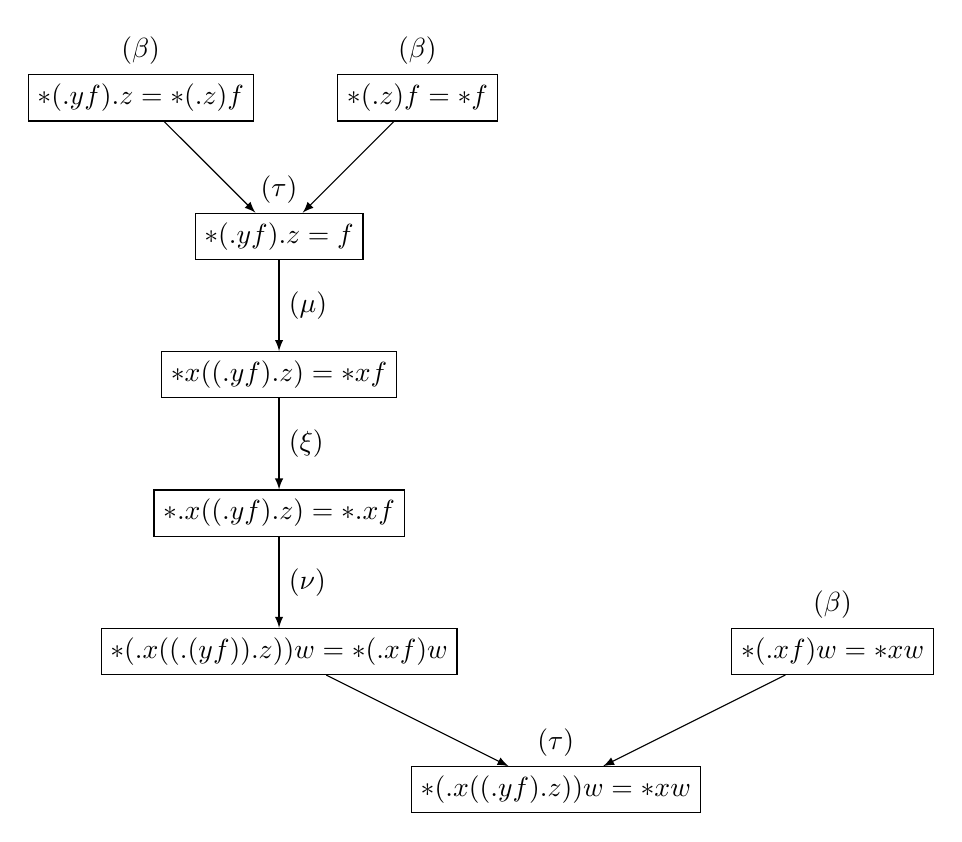
\begin{tikzpicture}[
    equat/.style={rectangle, draw},
    grow=up,
    edge from parent/.style={draw,latex-},
    level 1/.style={sibling distance=20em, level distance=5em},
    level 2/.style={sibling distance=40em},
    level 3/.style={sibling distance=20em},
    level 4/.style={sibling distance=10em}
    ]
    \node [equat] (foo1) {\(\lc*{(\f.x((\y.y f) \z.z))w} = \lc*{x w}\)}
    child {
      node [equat] (foo3) {\(\lc*{(\f.x f)w} = \lc*{x w}\)}
    }
    child {
      node [equat] (foo5) {\(\lc*{(\f.x((\y.(y f)) \z.z))w}=\lc*{(\f.x f)w}\)}
      child {
        node [equat] (foo7) {\(\lc*{\f.x((\y.y f)\z.z)}=\lc*{\f.x f}\)}
        child {
          node [equat] (foo9) {\(\lc*{x((\y.y f)\z.z)}=\lc*{x f}\)}
          child {
            node [equat] (foo11) {\(\lc*{(\y.y f)\z.z} = f\)}
            child {
              node [equat] (foo13) {\(\lc*{(\z.z)f} = \lc*{f}\)}
            }
            child {
              node [equat] (foo14) {\(\lc*{(\y.y f)\z.z} = \lc*{(\z.z)f}\)}
            }
            edge from parent [] node [right] {\((\mu)\)}
          }
          edge from parent [] node [right] {\((\xi)\)}
        }
        edge from parent [] node [right] {\((\nu)\)}
      }
    };
    \node [above=0em of foo13] (bar1) {\((\beta)\)};
    \node [above=0em of foo14] (bar2) {\((\beta)\)};
    \node [above=0em of foo11] (bar3) {\((\tau)\)};
    \node [above=0em of foo1] (bar4) {\((\tau)\)};
    \node [above=0em of foo3] (bar5) {\((\beta)\)};
  \end{tikzpicture}
\end{figure}

Tres términos lambda de suma importancia son:

\begin{itemize}
\item \(\lc{q[bold[I]]} \synteq \lc*{\x.x}\);
\item \(\lc{q[bold[K]]} \synteq \lc*{\x y.x}\);
\item \(\lc{q[bold[S]]} \synteq \lc*{\x y z.x z(y z)}\).
\end{itemize}

\begin{cor}
  Para todo término \(\lc{M},\ \lc{N},\ \lc{L} \in \Lambda\)
  \begin{itemize}
  \item[(i)] \(\lc*{q[bold[I]] M} =_{\boldsymbol{\lambda}} M\)
  \item[(ii)] \(\lc*{q[bold[K]] M N} =_{\boldsymbol{\lambda}} M\)
  \item[(iii)] \(\lc*{q[bold[S]] M N L} =_{\boldsymbol{\lambda}} \lc*{M L(N L)}\)
  \end{itemize}
\end{cor}

Estos tres combinadores generan en la teoría \(\boldsymbol{\lambda}\) al
conjunto \(\Lambda^{0}\) utilizando únicamente aplicación de términos lambda.
Debido a que \(\lc*{q[bold[S K K]]}=_{\boldsymbol{\lambda}} \lc*{q[bold[I]]}\),
sólo es necesario considerar a \(\lc{q[bold[K]]}\) y a \(\lc{q[bold[S]]}\) para
generar a \(\Lambda^{0}\). \\

\subsubsection{Otras teorías}

En el artículo \cite{Church:LambdaConversion}, Alonzo Church presenta una
definición del cálculo lambda con un conjunto restringido de términos lambda. A
la teoría que considera a este conjunto restringido de términos lambda (denotado
\(\Lambda_{I}\)) y los axiomas  y reglas de inferencia de la teoría
\(\boldsymbol{\lambda}\) cambiando \(\Lambda\) por \(\Lambda_{I}\) se le conoce
como teoría \(\boldsymbol{\lambda I \beta}\) (o el cálculo \(\lambda I\)). \\

El conjunto \(\Lambda_{I}\) se define de manera inductiva como
\begin{itemize}
\item \(\lc{x} \in \Lambda_{I}\);
\item \(\lc{M}\in \Lambda_{I},\ \lc{x} \in \lc{q[fv[M]]} \implies \lc{\x.M} \in
  \Lambda_{I}\);
\item \(\lc{M},\ \lc{N} \in \Lambda_{I} \implies \lc{M N} \in \Lambda_{I}\).
\end{itemize}

La diferencia fundamental entre las teorías \(\boldsymbol{\lambda K \beta}\) y
\(\boldsymbol{\lambda I \beta}\) es el término lambda \(\lc{q[bold[K]]}\), ya que
\(\lc{q[bold[K]]} \in \Lambda \setminus \Lambda_{I}\) pero \(\lc{q[bold[K]]}
\not\in \Lambda_{I}\). Esto es debido a que el subtérmino \(\lc{\y.x}\) en
\(\lc{q[bold[K]]}\synteq \lc{\x y.x}\) no puede existir en \(\Lambda_{I}\)
debido a que \(\lc{y} \not\in \lc{q[fv[x]]}\). \\




\subsubsection{Extensionalidad}

\subsubsection{Equivalencia de teorías}

\subsubsection{Lemas y Corolarios sobre términos lambda en \(\lambda K \beta\)}

\subsection{Teoría de reducción}

\subsubsection{Contracciones}

\subsubsection{Reducciones}

\subsubsection{Convertibilidad}

\subsubsection{Teorema de Church-Rosser}

\subsection{Böhm trees}

%%% Local Variables: 
%%% coding: utf-8 
%%% mode: latex
%%% TeX-master: "main"
%%% End:

\chapter{Codificación de objetos}
\section{Álgebra Booleana}

Uno de los atributos del cálculo lambda es que nos permite codificar información usando términos lambda y definir algoritmos utilizando reducciones que manipulen estos términos. Un buen ejemplo de esto es la  representación de valores de verdad, de los cuales podemos derivar las operaciones elementales del álgebra booleana. \\

Se establecen primero los cimientos de este sistema booleano primitivo determinando la representación de los valores \emph{verdadero} y \emph{falso}. Los algoritmos que se elaboran en esta subsección se basan en los términos que se les asocia a estos dos valores. \\

\subsection{Valores de verdad}

Es posible formular predicados lógicos con la notación del cálculo lambda. Se le asignan términos lambda a los valores de falso y verdadero. El término asociado a verdadero es \(\lc{\x y.x}\) y el término asociado a falso es \(\lc{\x y.y}\). \\

A partir de estos términos se pueden obtener nuevos términos lambda para los operadores básicos del álgebra booleana, para el resto de la sección se define \(\lc{q[bold[V]]} \synteq \lc*{\x y.x}\) (verdadero) y \(\lc{q[bold[F]]}\) (falso), es decir, \(\lc{q[bold[V]]}\) es una función de dos parámetros que al ser evaluada regresa el primer argumento y \(\lc{q[bold[F]]}\) es una función de dos parámetros que al ser evaluada regresa el segundo argumento. \\

\subsection{Conectivos lógicos}

Explorando con esta representación podemos obtener términos lambda obtenidos a partir de la aplicación de las combinaciones de estos dos valores. \\

Combinaciones de la aplicación de dos valores de verdad. \\

\begin{itemize}
\item \(\lc{q[bold[V]] q[bold[V]]}\)
  \begin{enumerate}
  \item \(\lc*{(\x y.x)(\x y.x)}\)
  \item \(\contract{\beta} \lc*{\y x w.x}\)
  \end{enumerate}
  Función de tres parámetros que al ser evaluada regresa el segundo argumento.
\item \(\lc{q[bold[V]] q[bold[F]]}\)
  \begin{enumerate}
  \item \(\lc*{(\x y.x)(\x y.y)}\)
  \item \(\contract{\beta} \lc*{\y x w.w}\)
  \end{enumerate}
  Función de tres parámetros que al ser evaluada regresa el tercer argumento.
\item \(\lc{q[bold[F]] q[bold[V]]}\)
  \begin{enumerate}
  \item \(\lc*{(\x y.y)(\x y.x)}\)
  \item \(\contract{\beta} \lc*{\y.y}\)
  \end{enumerate}
  Función de un parámetro que al ser evaluada regresa el argumento.
\item \(\lc{q[bold[F]] q[bold[F]]}\)
  \begin{enumerate}
  \item \(\lc*{(\x y.y)(\x y.y)}\)
  \item \(\contract{\beta} \lc*{\y.y}\)
  \end{enumerate}
  Función de un parámetro que al ser evaluada regresa el argumento
\end{itemize} \

Combinaciones de la aplicación de tres valores de verdad. \\

\begin{itemize}
\item \(\lc{q[bold[V]] q[bold[V]] q[bold[V]]}\)
  \begin{enumerate}
  \item \(\lc*{(\y x w.x)(\x y.x)}\)
  \item \(\contract{\beta} \lc*{\x w.x}\)
  \item \(\contract{\alpha} \lc{q[bold[V]]}\)
  \end{enumerate}
\item \(\lc{q[bold[V]] q[bold[V]] q[bold[F]]}\)
  \begin{enumerate}
  \item \(\lc*{(\y x w.x)(\x y.y)}\)
  \item \(\contract{\beta} \lc*{\x w.x}\)
  \item \(\contract{\alpha} \lc{q[bold[V]]}\)
  \end{enumerate}
\item \(\lc{q[bold[V]] q[bold[F]] q[bold[V]]}\)
  \begin{enumerate}
  \item \(\lc*{(\y x w.w)(\x y.x)}\)
  \item \(\contract{\beta} \lc*{\x w.w}\)
  \item \(\contract{\alpha} \lc{q[bold[F]]}\)
  \end{enumerate}
\item \(\lc{q[bold[V]] q[bold[F]] q[bold[F]]}\)
  \begin{enumerate}
  \item \(\lc*{(\y x w.w)(\x y.y)}\)
  \item \(\contract{\beta} \lc*{\x w.w}\)
  \item \(\contract{\alpha} \lc{q[bold[F]]}\)
  \end{enumerate}
\item \(\lc{q[bold[F]] q[bold[V]] q[bold[V]]}\)
  \begin{enumerate}
  \item \(\lc*{(\y.y)(\x y. x)}\)
  \item \(\contract{\beta} \lc*{\x y.x}\)
  \item \(\synteq \lc{q[bold[V]]}\)
  \end{enumerate}
\item \(\lc{q[bold[F]] q[bold[V]] q[bold[F]]}\)
  \begin{enumerate}
  \item \(\lc*{(\y.y)(\x y.y)}\)
  \item \(\contract{\beta} \lc*{\x y.y}\)
  \item \(\synteq \lc{q[bold[F]]}\)
  \end{enumerate}
\item \(\lc{q[bold[F]] q[bold[F]] q[bold[V]]}\)
  \begin{enumerate}
  \item \(\lc*{(\y.y)(\x y.x)}\)
  \item \(\contract{\beta} \lc*{\x y.y}\)
  \item \(\synteq \lc{q[bold[F]]}\)
  \end{enumerate}
\item \(\lc{q[bold[F]] q[bold[F]] q[bold[F]]}\)
  \begin{enumerate}
  \item \(\lc*{(\y.y)(\x y.y)}\)
  \item \(\contract{\beta} \lc*{\x y.x}\)
  \item \(\synteq \lc{q[bold[V]]}\)
  \end{enumerate}
\end{itemize} \

Un vistazo superficial a estas dos tablas me dice que nos será de más ayuda la segunda, ya que a partir de valores de verdad se obtienen otros valores de verdad. Si suponemos que hay dos predicados \(\lc{P}\) y \(\lc{Q}\) los cuales pueden tomar los valores \(\lc{q[bold[V]]}\) o \(\lc{q[bold[F]]}\), podemos ver estas combinaciones como \\

\begin{center}
 \begin{tabular}{|c|c|c|c|c|c|} 
 \hline
 \(\lc{P}\) & \(\lc{Q}\) & \(\lc{P P P}\) & \(\lc{P P Q}\) & \(\lc{P Q P}\) & \(\lc{P Q Q}\) \\ [0.5ex] 
 \hline\hline
 \(\lc{q[bold[F]]}\) & \(\lc{q[bold[F]]}\) & \(\lc{q[bold[F]]}\) & \(\lc{q[bold[F]]}\) & \(\lc{q[bold[F]]}\) & \(\lc{q[bold[F]]}\) \\ 
 \hline
 \(\lc{q[bold[F]]}\) & \(\lc{q[bold[V]]}\) & \(\lc{q[bold[F]]}\) & \(\lc{q[bold[V]]}\) & \(\lc{q[bold[F]]}\) & \(\lc{q[bold[V]]}\) \\
 \hline
 \(\lc{q[bold[V]]}\) & \(\lc{q[bold[F]]}\) & \(\lc{q[bold[V]]}\) & \(\lc{q[bold[V]]}\) & \(\lc{q[bold[F]]}\) & \(\lc{q[bold[F]]}\) \\
 \hline
 \(\lc{q[bold[V]]}\) & \(\lc{q[bold[V]]}\) & \(\lc{q[bold[V]]}\) & \(\lc{q[bold[V]]}\) & \(\lc{q[bold[V]]}\) & \(\lc{q[bold[V]]}\) \\ [1ex] 
 \hline
\end{tabular}
\end{center} \

\begin{itemize}
\item \(\lc{P P Q}\) o \(\lc{Q Q Q}\)
\item \(\lc{P P Q}\) o \(\lc{Q Q P}\)
\item \(\lc{P Q P}\) o \(\lc{Q P Q}\)
\item \(\lc{P Q Q}\) o \(\lc{Q P P}\)
\end{itemize} \

Teniendo en cuenta que el conjunto de valores que puede tomar \(\lc{P}\) es el mismo que puede tomar \(\lc{Q}\), solo consideramos una de las columnas. Se prosigue construyendo una tabla de verdad de estas cuatro posibilidades: \\

Por los valores de las tablas de verdad, encontramos que: \\

\[Conjuncion \synteq \lc{\p q.p q p}\] \

\[Disyuncion \synteq \lc{\p q.p p q}\] \

Con este procedimiento logramos obtener las operaciones booleanas básicas de conjunción (asociado a la compuerta lógica \(\mathrm{AND}\)) y disyunción (asociado a la compuerta lógica \(\mathrm{OR}\)). Para poder completar la incrustación del álgebra booleana en el cálculo lambda necesitamos poder representar la operación de negación, la cual derivaremos con otra metodología. \\

El término lambda que representa la negación debe ser una abstracción que tenga como parámetro un predicado \(p\) y que regrese un término de dos parámetros que regrese el primero si \(p\) es falso y el segundo si \(p\) es verdadero. La forma de éste término es \(\lc{\p x y.?}\) donde \(\lc{?}\) es un término por definir. Para encontrar este término incógnita hacemos la observación que si \(p\) es verdadero el primer argumento que le apliquemos será el resultado, mientras que si \(p\) es falso, el segundo argumento que le apliquemos será el resultado. Por lo tanto \\

\[\lc{(\p x y.p y x)q[bold[V]]} \contract{\beta} \lc*{\x y.y} \synteq \lc{q[bold[F]]}\] \

\[\lc{(\p x y.p y x)q[bold[F]]} \contract{\beta} \lc*{\x y.x} \synteq \lc{q[bold[V]]}\] \

Bajo este mismo procedimiento podemos encontrar otras operaciones útiles relacionadas con estructuras de control como condicionales. Para tener un término lambda de la condicional ``Si \(\lc{P}\) entonces \(\lc{M}\), de lo contrario \(\lc{N}\)'', donde \(\lc{P}\) es un valor de verdad con esta codificación y \(\lc{M}\) y \(\lc{N}\) son términos cualesquiera, se construye como \(\lc{\p m n.?}\), donde \(\lc{?}\) debe de resultar en \(m\) si \(p\) es verdadero y en \(n\) si \(p\) es falso. Por lo tanto \\

\[Condicional \synteq \lc{λp m n.p m n}\] \

Este término debe ser aplicado como \(\lc{Condicional Predicado Consecuente Contrario}\) para ser \(\beta\)-reducido de manera correcta. \\

Queda pendiente expandir el trabajo de lógica proposicional que se ha desarrollado a la admisión de mas de dos valores de verdad, buscando ser consistente con la metodología de derivación de términos utilizada. \\


\section{Aritmética}

Así como se pueden representar los valores de verdad de falso y verdadero en el cálculo lambda, también podemos encontrar representaciones para los números naturales. En esta sección se aborda una representación llamada numerales de Church, también se presentan términos lambda para operar números naturales con esta representación. \\

Para cada \( n \in \mathbb{N} \) el numeral de Church de \( n \) es un término lambda denotado como \( \lc{q[bar[n]]} \) definido como: \\

\[ \lc{q[bar[n]]} \synteq \lc{ λx y.q[left-apply[n,x,y]] } \] \

En la siguiente tabla se puede apreciar mejor la estructura de los numerales de Church: \\

\begin{center}
  \begin{tabular}{|c|c|}
    \hline
    \( n \) & \( \lc{q[bar[n]]} \) \\
    \hline
    0 & \( \lc*{λx y.y} \) \\
    \hline
    1 & \( \lc*{λx y.x y} \) \\
    \hline
    2 & \( \lc*{λx y.x(x y)} \) \\
    \hline
    3 & \( \lc*{λx y.x(x(x y))} \) \\
    \hline
    ... & ... \\
    \hline
  \end{tabular} \
\end{center} \

Como se observa en la tabla, un numeral de Church es una abstracción descurrificada de dos argumentos la cual al ser evaluada es reducida a la \( n \)-ésima composición del primer argumento evaluada en el segundo argumento. \\

Una manera de entender esta representación es pensar en los números naturales como un conteo de uno en uno; el 0 es no contar; el 1 es contar uno mas que el 0; el 2 es uno mas que el 1, así que el 2 es uno mas que el uno mas que el 0; el 3 es uno mas que el 2, así que el 3 es uno mas que el uno mas que el uno mas que el 0 y así sucesivamente. La idea de ``el uno mas'' es la del sucesor, si consideramos a \( x \) como una función sucesor y a \( y \) como el 0, podemos expresar \( x(x(x(y))) \) como \( sucesor(sucesor(sucesor(0))) \), así que: \\

\begin{align*}
sucesor(sucesor(sucesor(0))) & = sucesor(sucesor(1)) \\
                             & = sucesor(2) \\
                             & = 3
\end{align*} \

Es interesante pensar en diferentes maneras de expresar las operaciones mas elementales de la aritmétima como términos lambda que operen sobre esta representación. A continuación se presenta una exploración de los términos lambda correspondientes a algunas operaciones elementales de la aritmética: suma, multiplicación, exponenciación y resta. La suma es una repetición de la operación sucesor, la multiplicación una repetición de suma, la exponenciación una repetición de multiplicaciones y la resta una repetición de la operación predecesor. Esto nos lleva a identificar las operaciones de sucesor y predecesor como los algoritmos base para el resto de las operaciones primitivas. \\

El término \emph{sucesor} debe ser uno tal que al ser aplicado a un numeral \( \lc{q[bar[n]]} \) se pueda \( \beta \)-reducir al numeral \( \lc{q[bar[n+1]]} \). Considerando la definición de \( \lc{q[bar[n]]} \synteq \lc*{λx y.q[left-apply[n,x,y]]}\), lo que buscamos es una manera de agregarle una \( \lc{x} \) a la composición en el cuerpo de \( \lc{q[bar[n]]} \) para obtener \( \lc*{λx y.q[left-apply[n+1,x,y]]} \). Se construye este término considerando primero que será aplicado a un numeral: \\

\[ \lc{sucesor} \synteq \lc{λq[bar[n]].?} \] \

Además el resultado de \( \beta \)-reducir esta aplicación deberá ser una función de dos argumentos (como lo son todos los numerales de Church): \\

\[ \lc{sucesor} \synteq \lc{λq[bar[n]].λx y.?} \] \

Tomando en cuenta que \( \lc{q[bar[n]] x y} \synteq \lc{q[left-apply[n,x,y]]} \) y que \( \lc{x q[left-apply[n,x,y]]} \synteq \lc{q[left-apply[n+1,x,y]]} \): \\

\[ \lc{sucesor} \synteq \lc{λn x y.x(n x y)} \] \

A continuación se \( \beta \)-reduce la aplicación de \( \lc{sucesor} \) al numeral \( \lc{q[bar[4]]} \synteq \lc{λx y.x(x(x(x y)))} \): \\

\begin{align*}
                & \lc{sucesor q[bar[4]]} \\
\synteq         & \lc*{(λn x y.x(n x y)) (λx y.x(x(x(x y))))} \\
\convertible{\alpha} & \lc*{(λn x y.x(n x y)) (λf z.f(f(f(f z))))} \\
\contract{\beta}    & \lc*{(λx y.x(((λf z.f (f (f (f z)))) x) y))} \\
\contract{\beta}    & \lc*{(λx y.x((λz.x(x(x(x z)))) y))} \\
\contract{\beta}    & \lc*{(λx y.x(x(x(x(x y)))))} \\
\synteq         & \lc*{q[bar[5]]}
\end{align*} \

La otra operación elemental en la aritmética es el \emph{predecesor}, el término que represente esta operación debe ser uno que cumpla con la siguiente definición: \\

\begin{align*}
\lc{predecesor q[bar[0]]} & \reduce{\beta} \lc{q[bar[0]]} \\
\lc{predecesor q[bar[n]]} & \reduce{\beta} \lc{q[bar[n-1]]}
\end{align*}

El término lambda del predecesor con la representación de numerales de Church es mucho mas compleja que la del sucesor. Se pudiera pensar que la misma idea utilizada en la derivación del sucesor aplicaría para la derivación del predecesor: si tenemos \( n \) aplicaciones de \( \lc{x} \) a \( \lc{y} \), al aplicar el término que buscamos a un numeral de Church se debe \( \beta \)-reducir a otro numeral con una aplicación de \( \lc{x} \) menos, se utiliza \( \lc{y} \) para añadir una \( \lc{x} \) mas en el cuerpo del numeral. Sin embargo, la estructura de los numerales no nos permite quitar una \( \lc{x} \) usando \( \lc{y} \) facilmente ya que el numeral puede ser aplicado a dos términos, el que representa las \( \lc{x} \) y el que representa a la \( \lc{y} \); la variable que determina el valor del numeral es  \( \lc{x} \) y la sustitución de \( \lc{x} \) por otro término en esta representación se hace con \emph{cada} aparición de \( \lc{x} \) en el cuerpo del numeral, por otro lado, al sustituír la \( \lc{y} \) por otro término solo podemos hacer mas complejo el término o sustituírla por otra variable. \\

Para derivar el término del predecesor vamos a presentar un término con una estructura similar a los numerales de Church: \\

\[ \lc*{λx y z.z q[left-apply[n,x,y]]} \] \

La diferencia entre este término y un numeral de Church es que podemos modificar su estructura por enfrente, por atrás y en las composiciones intermedias. Si este término representara \( \lc{q[bar[n+1]]} \) pudieramos obtener el cuerpo de \( \lc{q[bar[n]]} \) de la siguiente manera: \\

\begin{align*}
& \lc*{(λx y z.z q[left-apply[n,x,y]]) x y (λa.a)} \\
\contract{\beta} & \lc*{(((λy z.z q[left-apply[n,x,y]]) y) (λa.a))} \\
\reduce{\beta} & \lc*{((λz.z q[left-apply[n,x,y]]) (λa.a))} \\
\contract{\beta} & \lc*{(λa.a) q[left-apply[n,x,y]]} \\
\contract{\beta} & \lc*{q[left-apply[n,x,y]]}
\end{align*} \

Es decir, mantenemos las \( \lc{x} \) y la \( \lc{y} \) y le aplicamos a \( \lc{q[left-apply[n,x,y]]} \) el término lambda que representa a la función identidad. Esta manera conveniente de representar a los numerales resulta ser incompleta, ya que no se podrá obtener \( \lc{q[left-apply[n-1,x,y]]} \) a partir del resultado (ya que la \( \lc{z} \) no aparece en el término resultante). Sin embargo, si logramos tener un término que nos genera este término modificado pudiéramos realizar esta transformación dentro de la función predecesor sería mas fácil encontrar \( \lc{q[bar[n-1]]} \). \\

La estructura del sucesor sería: \\

\[ \lc{λn x y. ? (λa.a)} \] \

Donde \( \lc{?} \) debe ser tal que al \( \beta \)-reducirse resulte en un término con la forma \( \lc{λz.z q[left-apply[n-1,x,y]]} \). Es conveniente desmenuzar el problema de encontrar este término desconocido: primero sabemos que el numeral de Church \( \lc{q[bar[n]]} \) puede ser aplicado a dos términos y el primer término al que sea aplicado se sustituirá en todas las apariciones de \( \lc{x} \), como queremos que la \( \beta \)-reducción nos genere una función cuyo argumento sea la primer variable en la composición del numeral, tenemos que encontrar una manera de propagar un término de la forma \( \lc{λw.w q[left-apply[m,x,y]]} \) de tal manera que al aplicarle otro término nos resulte \( \lc{λw.w q[left-apply[m+1,x,y]]} \). De esta manera al aplicar este otro término una y otra vez, resulte \( \lc{λw.w q[left-apply[n-1,x,y]]} \) con el cual podemos obtener el cuerpo del predecesor sustituyendo \( \lc{w} \) por \( \lc{λa.a} \). \\

Este otro término que buscamos será el que sustituirá a la \( \lc{x} \) en \( \lc{q[bar[n]]} \) para que: \\

\[ \lc{? (λw.w q[left-apply[m,x,y]])} \reduce{\beta} \lc{λw.w q[left-apply[m+1,x,y]]}) \] \

Lo que sucede en cada aplicación de este estilo es que se compone una \( \lc{x} \) en cada aplicación y se deja explícita una \( \lc{w} \) que podrá ser sustituída como valor. El término que nos permite hacer esto tiene la siguiente forma: \\

\[ \lc{λg w.w (g x)} \] \

Al ser aplicado a un término \( \lc{λw.w q[left-apply[m,x,y]]} \) la variable \( \lc{g} \) será sustituída por este término y el resultado será \( \lc{λw.w((λr.r q[left-apply[m,x,y]]) x)} \) (nótese el cambio de nombre de la variable ligada \( \lc{w} \) en el argumento), lo cual se reduce a \( \lc{λw.w q[left-apply[m+1,x,y]]} \) el cual mantiene su estructura original. \\

El percance con esta aproximación a la solución es que el primer valor al que se le aplica el término \( \lc{λg w.w (g x)} \) debe ser \( \lc{λw.w y} \). \\

Para visualizar una manera de resolver el problema, es conveniente expresar cómo se verían las aplicaciones de \( \lc{λg w.w (g x)} \) para un numeral de Church en particular. Si consideramos la aplicación de \( \lc{q[bar[4]] (λg w.w(g x))} \): \\

\begin{align*}
& \lc{q[bar[4]] (λg w.w(g x))} \\
\synteq & \lc*{( (λx y.q[left-apply[4,x,y]]) (λg.(λw.(w (g x)))) )} \\
\synteq & \lc*{( (λx y.x(x(x(x y)))) (λg.(λw.(w (g x)))) )} \\
\contract{\beta} & \lc*{(λy.(λg.(λw.(w (g x))))((λg.(λw.(w (g x))))((λg.(λw.(w (g x))))((λg.(λw.(w (g x)))) y))))}
\end{align*} \

Esto nos lleva al segundo paso para encontrar la función predecesor, en el desarrollo anterior notamos que la primer aplicación de \( \lc{λg w.w (g x)} \) es en la variable \( \lc{y} \) la cual está ligada por la \( \lambda \) del término. Sabemos que para obtener \( \lc{λw.w q[left-apply[3,x,y]]} \) debemos \( \beta \)-reducir el término: \\

\[ \lc{((λg.(λw.(w (g x)))) ((λg.(λw.(w (g x)))) ((λg.(λw.(w (g x)))) (λw.w y))))} \] \

Con esto podemos encontrar el valor que tiene que tomar \( \lc{y} \) en el numeral ya que: \\

\[ \lc{((λg.(λw.(w (g x)))) y)} \reduce{\beta} \lc{λw.w y} \] \

El término que buscamos es el que debe sustituír a la variable \( \lc{y} \) en la reducción: \\

\begin{align*}
& \lc{((λg.(λw.(w (g x)))) ?)} \\
\reduce{\beta} & \lc{(λw.(w (? x)))}
\end{align*} \

El término \( \lc{?} \) debe ser una función que al ser aplicada a \( \lc{x} \) se reduzca a \( \lc{y} \). El término \( \lc{λu.y} \) cumple con esta propiedad y será el que utilizaremos. \\

Considerando los términos determinados en el procedimiento anterior, podemos decir cómo será la función predecesor. Primero se aplica \( \lc{(λg.(λw.(w (g x))))} \) a \( \lc{q[bar[n]]} \), este término resultante se aplica a \( \lc{λu.y} \), \( \beta \)-reducir esta aplicación nos resulta \( \lc{λw.w q[left-apply[n-1,x,y]]} \) la cual puede ser aplicada a la función identidad \( \lc{λa.a} \) para obtener \( \lc{q[left-apply[n-1,x,y]]} \). Lo cual nos lleva al término completo de predecesor: \\

\[ \lc{(λn.(λx y.(((n (λg.(λw.(w (g x))))) (λu.y)) (λa.a))))} \] \

Teniendo los términos lambda de sucesor y predecesor se puede abordar la derivación de operaciones mas complejas como la de adición, multiplicación, exponenciación y sustracción de numerales de Church siguiendo el mismo enfoque. En este trabajo no se abordan otras operaciones como la división debido al aumento de complejidad por no ser una operación interna, es decir, la división de dos naturales puede ser un racional y no se definió una representación de términos lambda para el conjunto de los racionales. \\

Un término lambda para la adición de dos numerales \( \lc{q[bar[m]]} \) y \( \lc{q[bar[n]]} \) es \\

\[ \lc{λm n.(λx y.n sucesor m)} \] \

y se obtuvo a partir de la observación de que realizar la suma \( m+n \) es equivalente a computar el \( n \)-ésimo sucesor de \( m \). \\

Utilizando la estructura de \( \lc{q[bar[n]]} \) podemos aplicar \( \lc{q[bar[n]] sucesor q[bar[m]]} \) para obtener la \( n \)-ésima composición de la función sucesor aplicada al numeral \( \lc{q[bar[m]]} \): \\

\begin{align*}
& \lc{ q[bar[n]] sucesor q[bar[m]]} \\
\synteq & \lc{(( (λx y.q[left-apply[n,x,y]]) sucesor) (λx y.q[left-apply[m,x,y]]))} \\
\contract{\beta} & \lc{( (λy. q[left-apply[n,sucesor,y]]) (λx y.q[left-apply[m,x,y]]))} \\
\contract{\beta} & \lc{q[left-apply[n,sucesor,λx y.q[left-apply[m,x,y]]]]} \\
\reduce{\beta} & \lc{λx y.q[left-apply[m+n,x,y]]} \\
\synteq & \lc{q[bar[m+n]]}
\end{align*} \

Un término lambda para la multiplicación de dos numerales de Church es \\

\[ \lc{λm n x y.n (m x) y} \] \

el cual aborda la idea de componer \( \lc{m n} \) consigo mismo \( n \) veces (lo cual equivaldría a sumar \( n \) veces \( m \). \\

En el caso de la adición y la multiplicación, el orden en el que aplicamos el término a los numerales no es de importancia ya que son operaciones conmutativas, \( m+n = n+m \) y \( m \times n = n \times m \). Sin embargo en la sustracción y la exponenciación no se tiene esta propiedad, por lo que es importante el orden en el que se aplican los numerales a los términos, para ello consideraremos el orden como \( m-n \) y \( m^{n} \). \\

Basándonos en el término de la adición podemos obtener un término de la sustracción el cual es \\

\[ \lc{λm n x y.n predecesor m} \]. \

Ya que en la adición se dejó explícito el acto de aumentar \( m \) veces en 1 a \( n \), cambiamos el término de \( \lc{sucesor} \) por el de \( \lc{predecesor} \) y ahora se decrementa \( m \) veces en 1 a \( n \). \\

Un término lambda para la exponenciación es \\

\[ \lc{λm n.n m} \], \

es curioso tener una representación tan sencilla para una operación tan compleja como esta. A diferencia de los anteriores términos, al aplicarle a ésta exponenciación dos numerales, el numeral resultante tendrá las variables compuestas las variables que no se componen en las entradas, es decir, si \( \lc{q[bar[m]]} \synteq \lc{λf g.q[left-apply[m,f,g]]} \) y \( \lc{q[bar[n]]} \synteq \lc{λx y.q[left-apply[n,x,y]]} \), el resultado será \( \lc{q[bar[superscript[m,n]]]} \synteq \lc{λg y.q[left-apply[superscript[m,n],g,y]]} \). \\

Para corroborar que estas representaciones calculan de manera correcta la operación correspondiente para los numerales de Church se pueden realizar varias pruebas con diferentes numerales de entrada. En este trabajo no se desarrollarán ejemplos para estos términos. \\

Los mecanismos que hemos utilizado para derivar las operaciones se basan en construír términos que vayan transformando entradas con una estructura determinada de tal manera que nos acerquemos poco a poco al cálculo de la operación deseada; esta labor llega a ser bastante tediosa y carece de interés algorítmico. A continuación se presenta una manera mas interesante y elegante de abordar el problema de representar operaciones aritméticas. \\

Se introduce el término lambda que me permite generar hiperoperaciones aritméticas: \\

\[ \lc{λf u m n.n (λw.f m w) u} \] \

Abstracción de la noción de repetición sobre la estructura de un numeral, considerar propiedades de conmutatividad y asociatividad en operaciones. Abordar el problema del cómputo de operaciones inversas. Determinar un término que nos genere elementos de la secuencia de hiperoperaciones. \\

\section{Procesos recursivos}

Combinador Y, ordenes de evaluación, funciones recursivas. \\

Presentar una breve introducción sobre los combinadores y hablar del combinador \( \lc{q[bold[Y]]} \) y cómo nos permite expresar funciones recursivas en el cálculo lambda. \\

Como ejemplos prácticos de esta subsección sería adecuado desarrollar el término para el cálculo de factoriales o algúna otra función de una sola variable que transforme un numeral de Church en otro. También pudiera expandir la recursividad a términos multivariables currificados como la función Ackermann (abstracción a la generación de hiperoperaciones, ver \emph{The Book of Numbers} de Conway). \\

\section{Pares ordenados}

Construcción axiomática de pares ordenados, listas, \(n\)-tuplas, árboles y otras estructuras complejas. \\

Presentar la representación de pares ordenados para la construcción de estructuras mas complejas. \\

\[ Car(Cons(x,y)) = x \] \

\[ Cdr(Cons(x,y)) = y \] \

Esta sección es apropiada para comenzar a relacionar la teoría de autómatas, lenguajes regulares y libres de contexto con sistemas medianamente complejos que se pueden incrustar en el cálculo lambda sin modificar el sistema. Un problema pudiece ser el no determinismo, pero pudiera solventar esto con el desarrollo de operaciones funcionales sobre listas (map, filter, fold, etc). \\

%%% Local Variables:
%%% coding: utf-8
%%% mode: latex
%%% TeX-master: "main"
%%% End:

% \chapter{El cálculo lambda sin tipos}
% El cálculo lambda es un sistema formal originalmente creado por Alonzo Church en 1932 con la finalidad de expresar, manipular y estudiar funciones para el desarrollo de los fundamentos de la lógica y las matemáticas \cite[p.~248]{Church:FoundationsLogic}. A lo largo de la historia, este sistema se ha adaptado para el estudio de los fundamentos de la computación y como sustento teórico para el desarrollo de lenguajes de programación.

Tres características fundamentales del cálculo lambda son

\begin{itemize}
\item El lenguaje e interpretación de las expresiones
\item La manipulación y transformación de expresiones
\item Las nociones de equivalencia entre expresiones
\end{itemize}

En este capítulo se describen estas tres características del cálculo lambda de manera informal, enfatizando las diferencias sintácticas, conceptuales y operacionales entre este sistema, la matemática clásica y la lógica de primer orden.

El contenido de este capítulo está basado en los primeros dos capítulos del libro \emph{The Lambda Calculus, Its Syntax and Semantics} por H.P. Barendregt \cite{Barendregt:Bible}; los capítulos 1 y 3 del libro \emph{Lambda Calculus and Combinators, an Introduction} por J.R. Hindley y J.P. Seldin \cite{HindleySeldin:LambdaCalculusAndCombinators}; y la monografía titulada \emph{The Calculi of Lambda-Conversion} por Alonzo Church \cite{Church:LambdaConversion}.

En el estudio del cálculo lambda existen dos \emph{lenguajes}

\begin{itemize}
\item El lenguaje de las expresiones del sistema
\item El \emph{metalenguaje} que describe al cálculo lambda
\end{itemize}

El lenguaje de las expresiones es un \emph{lenguaje formal} que especifica las secuencias de símbolos que representan expresiones válidas del cálculo lambda, se relaciona con las clases de objetos del sistema que son válidos manipular, comparar y representar. Por otro lado, el metalenguaje es un lenguaje informal que permite describir \emph{cómo} es que estas expresiones son manipuladas y analizadas, así como los mecanismos para representar conceptos y objetos matemáticos como expresiones.

\section{Expresiones}
\label{sec:expresiones}

Existen tres clases de expresiones en el cálculo lambda: los \emph{átomos}, las \emph{abstracciones} y las \emph{aplicaciones}.

\subsection{Átomos}
\label{sec:atomos}

Las expresiones más simples son los \emph{átomos}, estos son objetos sintácticos usualmente representados con un símbolo como \( x \), \( y \) o \( z \). Los átomos son la representación simbólica de las variables \cite[p.~577]{Barendregt:Bible}.

Cuando se tiene una expresión que se conforma de varias \( x \) se refiere al símbolo como ``el átomo \( x \)'', sin embargo es posible tener diferentes variables representadas con el mismo símbolo en la expresión y para referirse a una de ellas en particular se debe especificar en que parte de la expresión se encuentra la variable \( x \) a la que se hace referencia.

Al igual que en la matemática clásica y en la lógica de primer orden, las variables más relevantes son las que se \emph{cuantifican}, por ejemplo en el estudio de funciones, la \( x \) en \( f(x) = M \) y en el estudio de enunciados lógicos, la \( y \) en \( \forall y\ M \) o \( \exists y\ M \).

En matemáticas y en computación es usual \emph{nombrar} valores, por ejemplo, declarar que \( x = 8 \) y expresar a \( x \) en diferentes contextos que no necesariamente son expresiones lógicas y funciones. En el cálculo lambda, los nombres son parte del metalenguaje y no del lenguaje de las expresiones.

\subsection{Abstracciones}
\label{sec:abstracciones}

Las abstracciones son expresiones con \emph{estructura}, es decir, se conforman de \emph{partes} identificables. Las expresiones que son abstracciones representan la generalización de una expresión y son usualmente asociadas al concepto de \emph{función}.

La definición de función en la matemática clásica es el de una relación entre un conjunto de entradas, llamado \emph{dominio} y un conjunto de salidas, llamado \emph{codominio}. Esta relación tiene además la propiedad de que cada elemento del dominio se asocia exactamente con un elemento del codominio, formalmente, sean \( A \) y \( B \) dos conjuntos, una función \( f \) con dominio \( A \) y codominio \( B \) es un subconjunto del producto cartesiano \( A \times B \), tal que para toda \( a \in A \), existe \( b \in B \) tal que \( (a,\ b) \in f \) y si \( (a,\ b^{\prime}) \in f \) con \( b^{\prime} \in B \), entonces \( b=b^{\prime} \).

Las funciones tienen varias maneras de ser representadas. En la definición anterior la representación es la de pares ordenados, en donde la primer componente del par es un elemento en el dominio y la segunda es un elemento en el codominio. Dependiendo del uso que se le dá a las funciones, puede ser conveniente representarlas simbólicamente con expresiones, gráficamente con dibujos, numéricamente con tablas o incluso verbalmente con palabras.

Las abstracciones en el cálculo lambda son representadas simbólicamente con un átomo y con otra expresión, se escriben de la forma \( (λx.M) \) donde \( x \) es algún átomo llamado variable enlazada o argumento y \( M \) es alguna expresión ya sea otra abstracción, una aplicación o un átomo a la cual llamamos cuerpo de la abstracción. Un ejemplo de abstracción es \( (λy.y) \) en donde el argumento y cuerpo de la abstracción son el átomo \( y \).

Además de la semejanza sintáctica con las funciones y las expresiones lógicas cuantificadas, las abstracciones proveen el mecanismo para asociarle un valor a una variable. Sin embargo, tanto las expresiones de funciones como las fórmulas lógicas están basadas en conjuntos y en operaciones sobre conjuntos: \( f(x)=M \) asocia a \( x \) un valor en el dominio de \( f \) en \( M \) y \( \exists x\ M \) asocia a \( x \) valores en el dominio del discurso en el enunciado \( M \). En contraste con el cálculo lambda, por definición no existen conjuntos, números, valores de verdad, ni cuantificadores lógicos en el lenguaje.

Es posible utilizar la definición de función para \emph{describir} operaciones y transformaciones de expresiones en el cálculo lambda, o utilizar lógica de primer orden para aseverar verdades en el sistema, o utilizar aritmética para cuantificar propiedades de las expresiones del cálculo lambda, sin embargo estos objetos matemáticos no están incrustados en el lenguaje de las expresiones y conforman lo que es el \emph{metalenguaje}.


\subsection{Aplicaciones}
\label{sec:aplicaciones}

Las aplicaciones, al igual que las abstracciones, son expresiones con estructura. Se conforman por otras dos expresiones y se escriben de la forma \( (M\, N) \) donde \( M \) y \( N \) son cualesquiera átomos, abstracciones o aplicaciones. Este tipo de expresiones son de cierta manera complementarias a las abstracciones ya que representan un potencial acto de concretar una expresión.

El concepto relacionado con las aplicaciones en la matemática clásica es el de \emph{aplicación de funciones}, sin embargo, en el cálculo lambda se hace una distinción entre la expresión sintáctica de una aplicación y el acto de ``evaluar'' una aplicación.

En el estudio de funciones, la aplicación de una función \( f \) en \( x \) se denota \( f(x) \) y es considerada igual al resultado de obtener el elemento del codominio de \( f \) a partir del valor de \( x \). Por ejemplo, considerando la función \( f(x)=x^{2} \), la expresión sintáctica de la aplicación de esta función a 8 es \( f(8) \), mientras que el valor de la evaluación de esta aplicación es 64. La notación de una abstracción del cálculo lambda es similar a la notación de aplicación de funciones, pero con el paréntesis abierto antes del nombre de la función, es decir, \( (f\, x) \) en lugar de \( f(x) \).

En el cálculo lambda, el concepto relacionado con la evaluación de funciones es el de \emph{reducción} de expresiones. En particular cuando se tiene la aplicación de una abstracción \( (λx.M) \) en algúna expresión \( N \), se dice que \( ((λx.M) N) \) se \emph{reduce} a una expresión \( Z \) la cual es similar a \( M \) solo que con \( x \) cambiada por \( N \). En la evaluación de funciones, el procedimiento es parecido, por ejemplo \( f(3) \) donde \( f = 2x^{2}+x-8 \), se evalúa sustituyendo las \( x \) de \( 2x^{2}+x-8 \) por 3, obteniendo así la expresión aritmética \( 2(3)^{2}+3-8 \), la cual puede ser operada para obtener el resultado 13.

Las abstracciones y aplicaciones del cálculo lambda son en algunos aspectos más restrictivos que las funciones y la aplicación de funciones. La función considera dos conjuntos cualquiera y no importa que propiedades tengan sus elementos o que operaciones se pueden realizar sobre ellos. Por otro lado, las abstracciones y aplicaciones sólo pueden ser descritas a partir de otras expresiones del cálculo lambda.

\subsection{Extensiones}
\label{sec:extensiones}

Cuando se desea representar en el cálculo lambda alguna función, se deben \emph{codificar} como expresiones del lenguaje los elementos del dominio y el codominio de la función, así como las operaciones entre elementos de ambos conjuntos. Por ejemplo, para representar la función \( f \colon \mathbb{N} \to \mathbb{N} \) dada por \( f(x)=x^{2} \) primero se deben codificar los números naturales con expresiones del cálculo lambda, esta codificación debe ser acompañada de la codificación de las operaciones aritméticas elementales como la suma y resta así como de los predicados sobre números naturales como discriminar entre el mayor de dos números o si un número es cero; posteriormente se debe expresar la operación de exponenciación de cualquier número natural como base y el número \( 2 \) como exponente. La codificación es similar a la implementación de algoritmos y estructuras de datos en lenguajes de programación.

El hecho de tener un lenguaje tan reducido y minimalista para las expresiones del cálculo lambda nos obliga a entender con detalle y precisión todos los procesos de manipulación y transformación de expresiones y siendo que todo lo que se representa con el cálculo lambda debe ser codificado como expresiones, los objetos representados pueden ser entendidos de la misma manera.

\subsection{Ejemplos}
\label{sec:ejemplos}

Con solo átomos, aplicaciones y abstracciones se pueden formular expresiones complejas. A continuación se presentan seis ejemplos de expresiones del cálculo lambda y se describen diferentes maneras en las cuales estas se pueden componer para formar otras expresiones más complejas.

\begin{exmp}
  Algunas expresiones del cálculo lambda
  \label{exmp:expresiones}
  \begin{subequations}
    \begin{gather}
      \label{eq:expresiones:a} \tag{a}
      x \\
      \label{eq:expresiones:b} \tag{b}
      (λx.x) \\
      \label{eq:expresiones:c} \tag{c}
      (y(λx.x)) \\
      \label{eq:expresiones:d} \tag{d}
      ((λy.(y(λx.x)))(λw.w)) \\
      \label{eq:expresiones:e} \tag{e}
      (λx.(x x)) \\
      \label{eq:expresiones:f} \tag{f}
      (λf.(λx.(f(f x))))
    \end{gather}
  \end{subequations}
\end{exmp}


Los átomos por si solos son expresiones válidas, en el inciso \eqref{eq:expresiones:a} aparece el átomo \( x \), como tal no tiene mucha utilidad, no podemos decir que toma valores en algún conjunto o que representa algún valor en particular como falso o verdadero, es tan sólo un símbolo. Al ser parte de otra expresión, un átomo puede tener más relevancia, en el inciso \eqref{eq:expresiones:b} el átomo \( x \) es el cuerpo de la abstracción \( (λx.x) \) y ahora tiene el potencial de ser cambiado por cualquier otra expresión debido a que también es el argumento.

En el inciso \eqref{eq:expresiones:c} se tiene la aplicación del átomo \( y \) en la abstracción del inciso \eqref{eq:expresiones:b}. A pesar de ser contraintuitivo, las expresiones de aplicación se componen de dos expresiones cualesquiera, por lo tanto, a pesar de estar asociada conceptualmente con la aplicación de funciones, la expresión \( (y (λx.x)) \) es válida. La expresión del inciso \eqref{eq:expresiones:d} contiene la expresión anterior en una abstracción en la primer parte de la aplicación y nos permite observar dos ideas importantes: primero, las abstracciones pueden ser aplicadas a abstracciones; segundo, al reducir la aplicación de \( (λy.(y(λx.x))) \) a \( (λw.w) \), el átomo \( y \) es cambiado por la expresión \( (λw.w) \), el resultado puede ser reducido nuevamente para obtener la expresión \( (λx.x) \).

\begin{exmp}
  Procedimiento de reducir la aplicación de \( (λy.(y (λx.x))) \) en \( (λw.w) \)
  \label{exmp:aplicacion}
  \begin{align*}
    \text{1. } & ((λy.(y (λx.x)))(λw.w)) & \text{expresión del inciso \eqref{eq:expresiones:d}} \\
    \text{2. } & ((λw.w)(λx.x)) & \text{al aplicar \( (λy.(y (λx.x))) \) a \( (λw.w) \)} \\
    \text{3. } & (λx.x) & \text{al aplicar \( (λw.w) \) a \( (λx.x) \)}
  \end{align*}
\end{exmp}

En el inciso \eqref{eq:expresiones:e} se presenta una abstracción cuyo cuerpo es la aplicación de su argumento sobre sí mismo. Lo interesante de esta expresión es que es que encapsula la idea de replicar cualquier expresión a la que sea aplicada. Por ejemplo, si aplicamos \( (λx.(x\, x)) \) al átomo \( y \) y se realiza el procedimiento de reducción como en el ejemplo \ref{exmp:aplicacion}, se obtiene \( (y\, y) \) y en general al realizar la reducción de \( ((λx.(x\, x))M) \) donde \( M \) es cualquier expresión, se obtiene \( (M\, M) \). Con esta expresión se puede formular una expresión auto-replicante en el cálculo lambda:

\begin{exmp}
  Procedimiento de reducir la aplicación de \( (λx.(x\, x)) \) en \( (λx.(x\, x)) \)
  \label{exmp:aplicacion2}
  \begin{align*}
    \text{1. } & ((λx.(x\, x))(λx.(x\, x))) & \text{expresión del inciso \eqref{eq:expresiones:e} aplicada a sí misma} \\
    \intertext{En \( (x\, x) \) de la expresión izquierda se cambia cada \( x \) por \( (λx.(x\, x)) \)}
    \text{2. } & ((λx.(x\, x))(λx.(x\, x))) & \text{resultado de la reducción.}
  \end{align*}
\end{exmp}

A este tipo de expresiones se les llaman ``quines'' \cite[pp.~431--437]{Hofstadter:GEB} término originalmente asociado a una paradoja sobre sistemas lógicos \cite{Quine:Paradox}. En la actualidad, el término ``quine'' hace referencia a un programa cuya \emph{salida} es el programa mismo.

En el inciso \eqref{eq:expresiones:f} se tiene una abstracción cuyo cuerpo es otra abstracción. El concepto interesante que ilustra esta expresión es el de representación de abstracciones de varias variables. Al reducir la aplicación de \( (λf.(λx.(f(f\, x)))) \) en una expresión cualquiera \( M \), se obtiene \( (λx.(M(M\, x))) \). Si posteriormente se reduce la aplicación de este resultado a una expresión cualquiera \( N \) se obtiene \( (M(M\, N)) \). El resultado final es similar al resultado que se obtendría al evaluar en \( M \) y \( N \) una función \( g(f,x) = f(f(x)) \), es decir, \( g(M,N) = M(M(N)) \).

Una manera de codificar funciones de varias variables como abstracciones del cálculo lambda es codificar a \emph{tuplas} o \emph{secuencias} y poder hacer referencia a sus elementos de manera individual, sin embargo, representar secuencias es un procedimiento más complejo que se aborda en la sección \ref{sec:pares-ordenados}.

\section{Operaciones}
\label{sec:operaciones}

En el cálculo lambda se pueden realizar algunas operaciones para transformar expresiones, estas operaciones son parte del metalenguaje y consisten de una serie de cambios mecánicos a la estructura de las expresiones de acuerdo a un criterio particular.

En la sección \ref{sec:expresiones} se describió de manera tangencial el acto de \emph{reducir} una aplicación basándonos en la noción de \emph{cambiar} una expresión por otra, en esta sección se describen operaciones basadas en esta misma noción.

\subsection{Sustitución}
\label{sec:op-sustitucion}

La \emph{sustitución} es la operación que nos permite transformar una expresión cualquiera \( M \) cambiando las apariciones de un átomo \( x \) por alguna otra expresión \( M \), este procedimiento se denota

\[ \subst{M}{x}{N} \]

En muchos casos la operación de sustitución se puede realizar de fácilmente:

\begin{exmp}
  Sustituciones sencillas
  \label{exmp:sustituciones}
  \begin{align}
    \label{eq:sustituciones:a} \tag{a}
    \subst{x}{x}{y} & = y \\
    \label{eq:sustituciones:b} \tag{b}
    \subst{(x(x(λy.y)))}{x}{z} & = (z(z(λy.y))) \\
    \label{eq:sustituciones:c} \tag{c}
    \subst{\subst{(((w\, x)y)z)}{x}{a}}{y}{b} & = (((w\, a)b)z) \\
    \label{eq:sustituciones:d} \tag{d}
    \subst{(x\, x)}{x}{(λw.w)} & = ((λw.w)(λw.w))
  \end{align}
\end{exmp}

Existen algunos detalles sutiles de la sustitución que se deben tomar en cuenta para evitar obtener expresiones erróneas, en particular cuando se sustituye en expresiones que contienen abstracciones. Para ilustrar estos casos especiales, consideremos la abstracción lambda análoga a una función constante \( (λx.y) \), en donde reducir la aplicación de ésta en cualquier otra expresión, resulta siempre en el átomo \( y \). Si se realiza la sustitución \( \subst{(λx.y)}{y}{z} \) se obtiene la expresión \( (λx.z) \) la cual también es análoga a una función constante pero con el átomo \( z \). Si no se tiene cuidado, sustituir un átomo por otro en esta abstracción puede resultar en una expresión con diferente \emph{interpretación}.

\begin{exmp}
  Caso patológico de la sustitución ingenua
  \label{exmp:sustitucion3}

  \[ \subst{(λx.y)}{y}{x} \]

  Se puede pensar que el resultado es \( (λx.x) \) la cuál es análoga a la función identidad, sin embargo, la sustitución no permite cambiar las expresiones de esta manera.
\end{exmp}

Para entender la operación de sustitución se tiene que pensar que lo que le da sentido a una variable \( x \) es una \( λ x \). Consideremos la expresión

\[ (λx.(λy.((x\, y)z))) \]

el átomo \( x \) que aparece en el cuerpo de la expresión se dice ser una variable \emph{ligada} a la \( λ x \), la cual se puede pensar como una especie de ``referencia'' a la expresión a la que la abstracción es aplicada, esto limita a la operación de sustitución a no \emph{romper} la referencia de una variable ligada. De igual manera, el átomo \( y \) es una variable ligada a la \( λ y \) y debe mantener su referencia bajo la operación de sustitución. Sin embargo, el átomo \( z \) es lo que se llama variable \emph{libre}: No está en el \emph{alcance} de alguna \( λ z \) y puede ser libremente sustituida por alguna otra expresión.

En el ejemplo \ref{exmp:sustitucion3} se pretende sustituir la variable libre \( y \) por una expresión \( x \), lo cual no debería presentar problemas, sin embargo, una sustitución tal cual de \( y \) por \( x \) \emph{introduciría} una referencia a la \( λ x \) de la expresión, la cuál no existía previamente. Con esto se identifica que la operación de sustitución \( \subst{M}{x}{N} \) no debe introducir o eliminar referencias a alguna \( λ \) en \( M \).

\subsection{Cambio de variable ligada}
\label{sec:op-cambio-var-ligada}

Para resolver el problema presentado en el ejemplo \ref{exmp:sustitucion3} se debe considerar otra operación llamada \emph{cambio de variable ligada}. Se parte de la observación que en una expresión del cálculo lambda, las referencias entre \( λ x \) y las variables \( x \) son más importantes que el símbolo con el que se representa el átomo. En las expresiones simbólicas de funciones sucede lo mismo, al expresar \( f(x)=x^{2} \) y \( f(y)=y^{2} \) hacemos referencia a la misma regla de correspondencia y por lo tanto a la misma función (sin considerar el dominio y el codominio de \( f \)). En el cálculo lambda, cambiar el símbolo que representa el átomo \( x \) en la expresión \( (λx.y) \) por otro símbolo no utilizado como \( z \) nos permite realizar la sustitución sin problemas.

\begin{exmp}
  Procedimiento de sustitución para el ejemplo \ref{exmp:sustitucion3}
  \label{exmp:sustitucion4}
  \begin{align*}
    \text{1. } & \subst{(λx.y)}{y}{x} & \\
    \text{2. } & \subst{(λz.y)}{y}{x} & \text{después de realizar un cambio de variable ligada} \\
    \text{3. } & (λz.x) & \text{resultado del procedimiento de sustitución}
  \end{align*}
\end{exmp}

Cuando se realiza un cambio de variable ligada sobre una abstracción \( (λx.M) \) se cambia tanto el átomo \( x \) acompañado por la \( λ \), llamada variable \emph{enlazada} como todas las apariciones del átomo en el cuerpo de la abstracción, también llamado \emph{alcance de} \( λ x \) a menos que en \( M \) se encuentre una expresión de la forma \( (λx.N) \), ya que las \( x \) en \( N \) hacen referencia a la \( λx \) de \( (λx.N) \) no de \( (λx.M) \).

En el ejemplo \ref{exmp:sustitucion4} el cambio de variable ligada únicamente cambió la variable enlazada, en otras expresiones el cambio de variable ligada puede realizarse múltiples veces para transformar varias abstracciones.

\begin{exmp}
  Múltiples cambios de variable ligada
  \label{exmp:variableligada}
  \begin{align*}
    \text{1. } & (λf.(λx.(f(f(f\, x))))) & \\
    \text{2. } & (λg.(λx.(g(g(g\, x))))) & \text{Cambiando \( f \) por \( g \)} \\
    \text{3. } & (λg.(λy.(g(g(g\, y))))) & \text{Cambiando \( x \) por \( y \)}
  \end{align*}
\end{exmp}

El cambio de variable ligada en una abstracción \( (λx.M) \) de \( x \) a \( y \) resulta en la abstracción

\[ (λy.\subst{M}{x}{y}) \]

La definición de la operación de sustitución es recursiva y hace uso de la operación de cambio de variable ligada, considerando a \( x \), \( y \), \( z \) como átomos diferentes y \( M \), \( N \) y \( P \) como expresiones cualquiera:

\begin{itemize}
\item \( \subst{x}{x}{M} \) resulta en \( M \);
\item \( \subst{y}{x}{M} \) resulta en \( y \);
\item \( \subst{(M\, N)}{x}{P} \) resulta en \( (\subst{M}{x}{P} \subst{N}{x}{P}) \);
\item \( \subst{(λx.M)}{x}{N} \) resulta en \( (λx.M) \) debido a que las referencias a \( x \) no deben eliminarse;
\item \( \subst{(λy.M)}{x}{N} \) resulta en:
  \begin{itemize}
  \item \( (λy.M) \) cuando \( x \) no es una variable libre en \( M \),
  \item \( (λy.\subst{M}{x}{N}) \) cuando \( x \) es una variable libre en \( M \) pero \( y \) no es una variable libre en \( N \) debido a que esto introduciría una referencia a \( λ y \),
  \item \( (λz.\subst{\subst{M}{y}{z}}{x}{N}) \) cuando \( x \) es una variable libre en \( M \) y \( y \) es una variable libre en \( N \).
  \end{itemize}
\end{itemize}

\subsection{Reducción de aplicaciones}
\label{sec:op-reduccion}

La operación de \emph{reducción de aplicaciones} es el mecanismo mediante el cual se puede ``concretar'' una abstracción haciendo uso de otra expresión como valor de la variable enlazada. De la misma manera en como se efectúa la evaluación de funciones en la matemática clásica, el concretar una función consiste en sustituir todas las apariciones del argumento por el valor en el que la función es aplicada.

La definición de la reducción de la aplicación de \( (λx.M) \) en una expresión cualquiera \( N \) es

\[ \subst{M}{x}{N} \]

A continuación se presentan ejemplos de reducciones con los pasos de la transformación

\begin{exmp}
  Procedimiento de reducir la aplicación de \( (λx.x) \) en \( y \)
  \label{exmp:aplicacion6}
  \begin{align*}
    \text{1. } & ((λx.x) y) \\
    \text{2. } & \subst{x}{x}{y} \\
    \text{3. } & y
  \end{align*}
\end{exmp}

\begin{exmp}
  Procedimiento de reducir la aplicación de \( (λw.w) \) en \( x \) dentro de otra expresión
  \label{exmp:aplicacion7}
  \begin{align*}
    \text{1. } & (λx.((λw.w)x)) \\
    \text{2. } & (λx.\subst{w}{w}{x}) \\
    \text{3. } & (λx.x)
  \end{align*}
\end{exmp}

\begin{exmp}
  Procedimiento de múltiples reducciones
   \label{exmp:aplicacion8}
  \begin{align*}
    \text{1. } & (((λf.(λx.(f(f(f\, x))))) g) y) \\
    \text{2. } & ((λx.\subst{(f(f(f\, x)))}{f}{g}) y) \\
    \text{3. } & ((λx.(g(g(g\, x)))) y) \\
    \text{4. } & \subst{(g(g(g\, x)))}{x}{y} \\
    \text{5. } & (g(g(g\, y)))
  \end{align*}
\end{exmp}

El cálculo lambda es un sistema maleable y se permite definir operaciones arbitrarias sobre expresiones para estudiar como el sistema se comporta en diferentes contextos, por ejemplo, se puede considerar una operación similar a la sustitución que permite introducir referencias a una o más \( λ \) en una expresión, sin embargo, el presente trabajo está constituido para entender plenamente las ideas centrales del cálculo lambda haciendo solamente uso de las operaciones de \emph{sustitución}, \emph{cambio de variable ligada} y \emph{aplicación de abstracciones}.

\section{Equivalencias}
\label{sec:equivalencias}

El cálculo lambda se considera formalmente como una \emph{teoría ecuacional}, esto significa que los axiomas del sistema formal son ecuaciones que relacionan expresiones del lenguaje. Esto hace que el concepto de \emph{equivalencia} de expresiones sea de suma importancia.

Es tan relevante la formalización de las nociones de equivalencia que considerar alguna equivalencia entre dos expresiones que se escriben diferente puede cambiar por completo el sistema formal que se estudia. En el desarrollo histórico del cálculo lambda, el estudio de los criterios que permiten establecer que dos expresiones son equivalentes ha dado pie a una gran diversidad de variantes de la teoría original; es por ello que en la literatura se suele hablar de \emph{los cálculos lambda} y no únicamente de un cálculo lambda.

Como se aborda en la sección \ref{sec:operaciones}, con la operación de sustitución se puede transformar expresiones del cálculo lambda y definir otras operaciones como el cambio de variable ligada y la reducción de aplicaciones. Usualmente, las transformaciones de expresiones se pueden asociar a nociones de equivalencia. En terminología del cálculo lambda, las nociones de equivalencia entre expresiones son asociadas a la propiedad de \emph{convertibilidad}, la cual significa que si dos expresiones \( M \) y \( N \) son equivalentes en el sistema, es posible transformar \( M \) a \( N \) y viceversa por medio de un número finito de operaciones.

En esta sección se describen algunos criterios de equivalencia entre expresiones del cálculo lambda y las maneras en las que las equivalencias se relacionan entre sí.

\subsection{Equivalencia sintáctica}
\label{sec:equivalencia-sintactica}

La \emph{equivalencia sintáctica} es una relación binaria entre expresiones que no está asociada a una transformación. Se considera como una equivalencia trivial, ya que asevera la igualdad entre dos expresiones que son escritas exactamente igual, símbolo por símbolo a excepción de abusos de notación. Por ejemplo, la expresión \( \sin^{2}(x) \) es un abuso de notación de \( \left( \sin(x) \right)^{2} \) y ambas se consideran exactamente iguales. En el cálculo lambda, la equivalencia sintáctica es denotada como

\[ M \synteq N \]

cuando \( M \) es sintácticamente la misma expresión que \( N \).

Todos los cálculos lambda, al igual que la mayoría de los sistemas formales, comprenden la noción de equivalencia sintáctica. Sin embargo las equivalencias más interesantes son las que involucran transformaciones entre expresiones.

\subsection{\( α \)-convertibilidad}
\label{sec:alfa-convertibilidad}

La operación de cambio de variable ligada se relaciona con una equivalencia estructural entre dos expresiones. Cuando se realiza esta operación no se modifica la estructura de la expresión, únicamente se modifica el símbolo usado para representar un átomo.

Considerando la expresión análoga a la función identidad \( (λx.x) \) se observa que tiene la misma estructura que la abstracción \( (λy.y) \) y que \( (λz.z) \), estas tres representan el mismo concepto. De igual manera otras expresiones como \( ((x\, y)z) \) o \( (λw.x) \) son estructuralmente equivalentes a \( ((a\, b)c) \) y \( (λf.h) \) respectivamente. A pesar de que no se escriben sintácticamente igual, la correspondencia que hay entre las posiciones de los átomos en una y otra expresión nos permite considerarlas como equivalentes. Sin embargo, la operación de cambio de variable ligada no considera cambios de nombres a átomos que sean variables libres.

Esta relación de equivalencia es llamada \( α \)-convertibilidad y se denota como

\[ M \convertible{α} N \]

para dos expresiones del cálculo lambda \( M \) y \( N \) en donde a partir de un número finito de cambios de variables ligadas en \( M \) o parte de \( M \) y en \( N \) o parte de \( N \) se puedan obtener expresiones sintácticamente equivalentes.

\subsubsection{Índices de De Bruijn}

Una técnica utilizada por algoritmos que verifican si dos expresiones \( M \) y \( N \) son \( α \)-convertibles es la de \emph{índices de De Bruijn}, esta transformación cambia la aparición de átomos por números naturales que representan la ``distancia'' de los átomos a las \( λ \) que hacen referencia.

\begin{exmp}[índices de De Bruijn]
  \label{exmp:debrujn}
  \[ (λz.((λy.(y(λx.x)))(λx.(z\, x)))) \]
  
  Se escribe usando índices de De Bruijn como

  \[ λ (λ 1 (λ 1)) (λ 2\, 1) \]

  En la figura \ref{fig:debrujn} se puede observar de manera gráfica la transformación de una notación a otra para este ejemplo, visualizando las expresiones del cálculo lambda como árboles.
\end{exmp}

\begin{figure}
  \centering

  \begin{tikzpicture}[level/.style={sibling distance=60mm/#1}]
    \node [draw] (term) {\( (λz.((λy.(y (λx.x))) (λx.(z\, x)))) \)};
    \node [below of=term] (arrow1) {\( \Downarrow \)};
    \node [circle,draw,below of= arrow1] (z) {\( λ z \)}
      child {
        node [circle,draw] (a) {\( λ y \)}
        child {
          node [circle,draw] (c) {\( y \)}
        }
        child {
          node [circle,draw] (d) {\( λ x \)}
          child {
            node [circle,draw] (g) {\( x \)}
          }
        }
      }
      child {
        node [circle,draw] (b) {\( λ x \)} 
        child {
          node [circle,draw] (e) {\( z \)}
        } 
        child {
          node [circle,draw] (f) {\( x \)}
        }
      };
      \node [below=130pt of z] (arrow2) {\( \Downarrow \)};
      \node [circle,draw,below of= arrow2] (z2) {\( λ \)}
      child {
        node [circle,draw] (a2) {\( λ \)} 
        child {
          node [circle,draw] (c2) {\( 1 \)}
        }
        child {
          node [circle,draw] (d2) {\( λ \)} 
          child {
            node [circle,draw] (g2) {\( 1 \)}
          }
        }
      }
      child {
        node [circle,draw] (b2) {\( λ \)} 
        child {
          node [circle,draw] (e2) {\( 2 \)}
        }
        child {
          node [circle,draw] (f2) {\( 1 \)}
        }
      };
      \node [below=130pt of z2] (arrow3) {\( \Downarrow \)};
      \node [draw,below of=arrow3](bruijn) {\( λ (λ 1 (λ 1)) (λ 2\, 1) \)};
  \end{tikzpicture}
  
  \caption{Transformación gráfica del ejemplo \ref{exmp:debrujn}}
  \label{fig:debrujn}
\end{figure}

Una desventaja de utilizar la notación de De Bruijn es que ciertas expresiones del cálculo lambda no pueden ser escritas, en particular, los átomos no pueden ser variables libres para que esta notación pueda ser utilizada.

\subsection{\( β \)-convertibilidad}
\label{sec:beta-convertibildad}

Al igual que el cambio de variable ligada, la operación de reducción de aplicaciones es utilizada para describir una equivalencia entre expresiones. La idea básica de esta equivalencia consiste en observar que al aplicar una abstracción \( (λx.M) \) a una expresión \( N \), el resultado de su reducción siempre es el mismo. De manera similar a la aplicación de funciones, cuando se define una función \( f(x)=x^{2} \), la aplicación \( f(3) \) se suele igualar al resultado de la aplicación: \( f(3)=8 \).

Esta relación de equivalencia es llama \( β \)-convertibilidad y se denota como

\[ M \convertible{β} N \]

para dos expresiones \( M \) y \( N \) en donde a partir de un número finito de reducciones a aplicaciones, reducciones inversas y cambios de variable ligada en \( M \) o parte de \( M \) y \( N \) o parte de \( N \) se puedan obtener expresiones sintácticamente equivalentes.

El proceso inverso a la reducción de aplicaciones se puede ilustrar considerando la reducción de \( (((λg.(λy.(g (g (g\, y))))) f) x) \) a \( (f(f(f\, x))) \). No es posible reducir la segunda expresión a la primera, pero ya la segunda expresión es una reducción de la primera, ambas son \( β \)-convertibles:

\[ (f(f(f\, x))) \convertible{β} (((λg.(λy.(g (g (g\, y))))) f) x) \]

\subsection{Relaciones de equivalencia}
\label{sec:relaciones-de-equivalencia}

Todas las nociones de convertibilidad son relaciones de equivalencia, las cuales por definición cumplen con tres propiedades.

Sea \( \sim \) una relación de equivalencia

\begin{enumerate}[a.]
\item Toda expresión \( M \) es equivalente a sí misma, es decir, \( M \sim M \). \label{enum:rela:a}
\item Si una expresión \( M \) es relacionada con una equivalencia a otra expresión \( N \), entonces \( N \) también es relacionada a \( M \), es decir \( M \sim N \implies N \sim M \). \label{enum:rela:b}
\item Si una expresión \( M \) se relaciona con una equivalencia a otra expresión \( N \) y \( N \) se relaciona con la misma equivalencia a \( P \), entonces, \( M \) y \( P \) se relacionan con esta equivalencia, es decir, \( M \sim N,\ N \sim P \implies M \sim P \). \label{enum:rela:c}
\end{enumerate}

La equivalencia sintáctica corresponde al inciso \ref{enum:rela:a} de las propiedades de equivalencias mencionadas y es llamada propiedad de \emph{reflexividad}; al igual que la \( α \)-conversión y la \( β \)-conversión, la equivalencia sintáctica no está asociada a una regla de inferencia. En los incisos \ref{enum:rela:b} y \ref{enum:rela:c} se tienen inferencias que parten de expresiones equivalentes y basado en si estas expresiones son equivalentes o no, ciertas propiedades se deben cumplir. En el inciso \ref{enum:rela:b} la propiedad es llamada \emph{simetría}, mientras que en el inciso \ref{enum:rela:c} la propiedad es llamada \emph{transitividad}.

La \( α \)-conversión y la \( β \)-conversión fueron definidas como equivalencias independientes y su definición cumple con las tres propiedades mencionadas a pesar de ser definidas en base a un procedimiento y no en una regla declarativa, sin embargo, es deseable referirse a una sola equivalencia de expresiones que tenga las propiedades de \emph{reflexividad}, \emph{simetría} y \emph{transitividad} y posteriormente considerar otras reglas que la equivalencia deba de cumplir.

Al igual que Haskell Curry en \cite[p.~59]{Curry:CombinatoryLogicI} se utilizan las letras griegas \( α \) y \( β \) para referirse a las ecuaciones relacionadas con la \( α \)-conversión y \( β \)-conversión respectivamente y las letras \( ρ \), \( σ \) y \( τ \) para referirse a las propiedades de reflexividad, simetría y transitividad respectivamente, se retoma esta convención para elaborar la siguiente definición de una relación de equivalencia \( \sim \):

\begin{defn}[Ecuaciones de \( \sim \)]
  Las ecuaciones con \( \sim \) que se satisfacen para expresiones del cálculo lambda son
  \label{defn:sim}
  \begin{subequations}
    \begin{align}
      \label{sim:alpha} \tag{\( α \)}
      (λx.M) & \sim (λy.\subst{M}{x}{y}) \\
      \label{sim:beta} \tag{\( β \)}
      ((λx.M)N) & \sim \subst{M}{x}{N} \\
      \label{sim:rho} \tag{\( ρ \)}
      M & \sim M \\
      \label{sim:sigma} \tag{\( σ \)}
      M \sim N & \implies N \sim M \\
      \label{sim:tau} \tag{\( τ \)}
      M \sim N,\ N \sim P & \implies M \sim P
    \end{align}
  \end{subequations}
\end{defn}

Las ecuaciones en la definición \ref{defn:sim} son muy parecidas a las propiedades de la \( β \)-conversión, con la excepción de que la \( β \)-conversión relaciona expresiones en donde sus partes fueron transformadas y \( \sim \) no, por ejemplo

\[ (λf.((λx.(f\, x)) y)) \convertible{β} (λf.(f\, y)) \]

pero

\[ (λf.((λx.(f\, x)) y)) \nsim (λf.(f\, y)) \]

Para capturar la definición de \( β \)-convertibilidad con ecuaciones, es necesario definir a \( \sim \) en partes de una expresión. Las siguientes reglas, nombradas por Curry \cite[p.~59]{Curry:CombinatoryLogicI} como \( ν \), \( μ \) y \( ξ \), junto con las reglas de \(\sim\) completan la definición declarativa de \( β \)-convertibilidad:

\begin{defn}
  Reglas que debe cumplir \( \sim \) para ser \( \convertible{β} \)
  \label{defn:simbeta}
  \begin{subequations}
    \begin{align}
      \label{simbeta:nu} \tag{\( ν \)}
      M \sim N & \implies (M\, Z) \sim (N\, Z) \\
      \label{simbeta:mu} \tag{\( μ \)}
      M \sim N & \implies (Z\, M) \sim (Z\, N) \\
      \label{simbeta:xi} \tag{\( ξ \)}
      M \sim N & \implies (λx.M) \sim (λx.N)
    \end{align}
  \end{subequations}
\end{defn}

Con estas reglas y a partir de un razonamiento lógico, podemos demostrar la \( β \)-equivalencia entre dos expresiones.

\begin{exmp}
  Razonamiento para concluir que \( (λf.((λx.(f\, x)) y)) \convertible{β} (λf.(f\, y)) \)
  \label{exmp:razonamiento-sim}
  \begin{align*}
    \text{1. } & ((λx.(f\, x)) y) \convertible{β} (f\, y) & & \text{por \( β \)} \\
    \text{2. } & (λf.((λx.(f\, x)) y)) \convertible{β} (λf.(f\, y)) & & \text{por \( ξ \)}
  \end{align*}
\end{exmp}

Es posible incluir aún más reglas de equivalencia cuando se estudia el cálculo lambda, a pesar de poder trabajar con expresiones en este sistema a partir de equivalencias arbitrarias, usualmente cada regla de equivalencia se asocia con alguna argumentación basada en la noción de función.

Por ejemplo, se pueden considerar dos abstracciones diferentes \( (λx.M) \) y \( (λy.N) \) que al ser aplicadas a cualquier expresión \( Z \) sean \( β \)-convertibles a una misma expresión \( W \). Si se relacionan las abstracciones del cálculo lambda con funciones, es natural pensar que \( M \) y \( N \) sean equivalentes, ya que por definición, dos funciones \( f \) y \( g \) son equivalentes si para toda \( x \) en su dominio \( f(x)=g(x) \). Por ejemplo, las funciones \( f(n)=\sum_{i=0}^{n}i \) y \( g(n)=\frac{n(n+1)}{2} \) a pesar de describir dos procedimientos diferentes para el cálculo de la suma de los primeros \( n \) números naturales son ``funcionalmente'' equivalentes ya que para todo natural \( f(n)=g(n) \). Por otro lado, si se relacionan las abstracciones del cálculo lambda con algoritmos, \( M \) y \( N \) no pudieran ser consideradas equivalentes ya que en el estudio de la complejidad algorítmica, el énfasis en la comparación entre dos procedimientos no es las entradas y salidas, si no el proceso que describen. Por ejemplo, el algoritmo de ordenamiento \emph{merge sort} logra ordenar una secuencia de \( n \) números de menor a mayor en \( \mathcal{O}(n \log n) \) mientras que el algoritmo \emph{bubble sort} computa el mismo resultado pero en \( \mathcal{O}(n^2) \).  La equivalencia ``funcional'' se pudiera incluír en la definición de \( \sim \) añadiendo la siguiente regla:

\[ (M\, P) \sim (N\, P) \implies M \sim N \]

Con esto se termina la introducción informal al cálculo lambda, las ideas que se han manejado en esta sección son formalizadas y definidas de manera rigurosa en el capítulo \ref{ch:formalizacion}.

%%% Local Variables:
%%% mode: latex
%%% TeX-master: "main"
%%% End:


\chapter{Tipos en el cálculo lambda}
La noción de \emph{generalización} es de suma importancia en el estudio general de funciones, operaciones o transformaciones. Los predicados en la lógica de primer orden, las funciones en la matemática clásica, los algoritmos en la computación y las abstracciones en el cálculo $ λ $ pueden ser considerados como instancias del concepto de generalización para los sistemas de los que forman parte y en algunos casos son la motivación original para el desarrollo de las teorías que los fundamentan.

El estudio de las propiedades generales de las funciones es una de las motivaciones originales del cálculo $ λ $, sin embargo, este cálculo se formuló de tal manera que es posible abstraer de su propósito original y ser tratado meramente como un sistema formal \cite{Church:LambdaConversion}.

El presente capítulo presenta un tratamiento matemático del cálculo $ λ $ con el objetivo de formalizar las ideas presentes en el \autoref{ch:nocion-informal} y ahondar en el objeto de estudio de este cálculo.

En la primera sección se define el conjunto que tiene como elementos todas las expresiones válidas del cálculo, se presentan propiedades y criterios de clasificación de expresiones y finalmente se formaliza el concepto de sustitución; en la segunda sección se construye una teoría formal del cálculo $ λ $, en donde un conjunto de axiomas y reglas de inferencia permiten plantear razonamientos lógicos para demostrar propiedades del cálculo; finalmente en la tercera sección se formulan nociones de reducción para las expresiones del cálculo usando sistemas de reescritura.

El contenido de este capítulo está basado en los primeros cuatro capítulos del libro ``The Lambda Calculus, Its Syntax and Semantics'' de H.P. Barendregt \cite{Barendregt:Bible} y los capítulos 1, 3, 6, 7 y 8 del libro ``Lambda Calculus and Combinators, an Introduction'' de J.R. Hindley y J.P. Seldin \cite{HindleySeldin:LambdaCalculusAndCombinators} así como el artículo ``A Set of Postulates for the Foundation of Logic'' y la monografía ``The Calculi of Lambda-Conversion'' de Alonzo Church \cite{Church:FoundationsLogic,Church:LambdaConversion}.

%\section{\texorpdfstring{Términos $ \bs{λ} $}{Términos lambda}}
\section{Términos \texorpdfstring{$ \bs{λ} $}{lambda}}
\label{sec:terminos-lambda}

Los \emph{términos $ λ $} son la formalización de las expresiones descritas en la \autoref{sec:expresiones}. El conjunto de todos los términos $ λ $ es un lenguaje formal $ Λ $ en donde sus elementos son cadenas compuestas de símbolos de un alfabeto \cite{Hopcroft:Automata}.

El lenguaje $ Λ $ se puede definir de diferentes maneras, a continuación se presenta una definición inductiva y posteriormente una definición basada en una gramática libre de contexto. En estas definiciones formales es común encontrar diferentes tipos de ``flechas'' que denotan diferentes cosas, en este trabajo se utiliza la flecha $ \implies $ para denotar una implicación lógica, $ \longrightarrow $ para denotar una producción en una gramática y $ \Rightarrow $ para denotar un paso en la derivación de una cadena.

\begin{defn}[Términos $ λ $]
  El conjunto $ Λ $ tiene elementos que son cadenas conformadas por símbolos en el alfabeto $ Σ=\{\mathtt{(},\ \mathtt{)},\ \mathtt{.},\ λ\} \cup V $, donde $ V $ es un conjunto infinito numerable $ \{v_{0},\ v_{00},\ v_{000},\ ... \} $ de variables. $ Λ $ es el conjunto más pequeño que satisface:
  \label{defn:terminos}
  \begin{subequations}
    \begin{align}
      \label{terminos:atomos}
      x \in V & \implies x \in Λ \\
      \label{terminos:abstracciones}
      M \in Λ,\ x \in V & \implies (λx.M) \in Λ \\
      \label{terminos:aplicaciones}
      M,\ N \in Λ & \implies (M\, N) \in Λ
    \end{align}
  \end{subequations}
\end{defn}

Cada parte de esta definición corresponde a las tres clases de término $ λ $:

\begin{description}
\item[\eqref{terminos:atomos}] establece que todo elemento de $ V $ es un término $ λ $ a los cuales se les llama \emph{átomos};
\item[\eqref{terminos:abstracciones}] establece que las cadenas de la forma $ (λx.M) $ son términos $ λ $, donde $ x $ es un átomo y $ M $ es cualquier término $ λ $, a estos términos se les llama \emph{abstracciones};
\item[\eqref{terminos:aplicaciones}] establece que las cadenas de la forma $ (M\, N) $ son términos $ λ $, donde $ M $ y $ N $ son términos $ λ $ cualesquiera, a estos términos se les llama \emph{aplicaciones}.
\end{description}

En el estudio usual de lenguajes formales \cite{Hopcroft:Automata}, $ Λ $ pertenece a la clase de lenguajes libres de contexto y puede ser definido de la siguiente manera:

\begin{defn}[Términos $ λ $]
  \label{defn:terminos-cfg}
  El conjunto de términos $ λ $ es el lenguaje generado por la gramática libre de contexto $ G $ conformado por las \emph{categorías sintácticas} $ T $, $ E $, $ F $ y $ A $, las cuales denotan las reglas para derivar términos $ λ $, aplicaciones, abstracciones y átomos respectivamente; los \emph{símbolos terminales} $ \{(,\ ),\ .,\ λ,\ v,\ {}_{0}\} $, los cuales son los símbolos que conforman a las cadenas en $ Λ $; el \emph{símbolo inicial} $ T $, el cual es el símbolo del que se derivan todos los términos $ λ $. Las reglas de producción de $ G $ son:
  \begin{subequations}
  \begin{align}
    \label{terminos-cfg:terminos}
    T & \rightarrow E\ \mid\ F\ \mid\ A \\
    \label{terminos-cfg:atomos}
    A & \rightarrow v_{0}\ \mid\ A {}_{0} \\
    \label{terminos-cfg:abstracciones}
    F & \rightarrow ( λ\ A\ .\ T\ ) \\
    \label{terminos-cfg:aplicaciones}
    E & \rightarrow (\ T\ T\ )
    \end{align}
  \end{subequations}
\end{defn}

Dada una secuencia de símbolos $ M $, se pueden utilizar estas dos definiciones para verificar si $ M $ es o no un término $ λ $. En el caso de la definición inductiva, se debe presentar un razonamiento que pruebe que las partes de la cadena satisface la \autoref{defn:terminos}. En el caso de la gramática libre de contexto de la \autoref{defn:terminos-cfg} se debe presentar una derivación de la cadena a partir de la categoría sintáctica $ T $.

A continuación se considera un ejemplo en donde una cadena de símbolos es elemento de $ Λ $. Sea $ M = (λv_{0}.(v_{00} (λv_{00}.v_{000}))) $, la cadena $ M $ es un término $ λ $ ya que

  \begin{description}
  \item[Por definición inductiva]
    \begin{align*}
      v_{000} \in V &\implies v_{000} \in Λ; \\
      v_{00} \in V,\ v_{000} \in Λ &\implies (λv_{00}.v_{000}) \in Λ,\ v_{00} \in Λ; \\
      v_{00},\ (λv_{00}.v_{000}) \in Λ &\implies (v_{00} (λv_{00}.v_{000})) \in Λ; \\
      v_{0} \in V,\ (v_{00} (λv_{00}.v_{000})) \in Λ &\implies (λv_{0}.(v_{00} (λv_{00}.v_{000}))).
    \end{align*}
  \item[Por gramática] Se mantienen los espacios en los lados derechos de las producciones de la gramática para ser consistentes, sin embargo, el espacio en blanco no es un símbolo terminal, por lo tanto pueden ser omitidos.
    \begin{align*}
      T &\Rightarrow F \Rightarrow (\ λ\ A\ .\ T\ ) \Rightarrow (\ λ\ v_{0}\ .\ T\ ) \Rightarrow (\ λ\ v_{0}\ .\ E\ ) \Rightarrow (\ λ\ v_{0}\ .\ (\ T\ T\ )\ ) \\
        &\Rightarrow (\ λ\ v_{0}\ .\ (\ A\ T\ )\ ) \Rightarrow (\ λ\ v_{0}\ .\ (\ A_{0}\ T\ )\ ) \Rightarrow (\ λ\ v_{0}\ .\ (\ v_{00}\ T\ )\ ) \\
        &\Rightarrow (\ λ\ v_{0}\ .\ (\ v_{00}\ F\ )\ ) \Rightarrow (\ λ\ v_{0}\ .\ (\ v_{00}\ (\ λ\ A\ .\ T\ )\ )\ ) \\
        &\Rightarrow (\ λ\ v_{0}\ .\ (\ v_{00}\ (\ λ\ A_{0}\ .\ T\ )\ )\ ) \Rightarrow (\ λ\ v_{0}\ .\ (\ v_{00}\ (\ λ\ v_{00}\ .\ T\ )\ )\ ) \\
        &\Rightarrow (\ λ\ v_{0}\ .\ (\ v_{00}\ (\ λ\ v_{00}\ .\ A\ )\ )\ ) \Rightarrow (\ λ\ v_{0}\ .\ (\ v_{00}\ (\ λ\ v_{00}\ .\ A_{0}\ )\ )\ ) \\
        &\Rightarrow (\ λ\ v_{0}\ .\ (\ v_{00}\ (\ λ\ v_{00}\ .\ A_{00}\ )\ )\ ) \Rightarrow (\ λ\ v_{0}\ .\ (\ v_{00}\ (\ λ\ v_{00}\ .\ v_{000}\ )\ )\ ).
    \end{align*}
  \end{description}

Al considerar una cadena que no es elemento de $ Λ $ se sigue un procedimiento similar. Sea $ N = ((λv_{00}.v_{0}\, v_{00}) v_{0}) $, la cadena $ N $ no es un término $ λ $ ya que

\begin{description}
\item[Por definición inductiva] Ya que $ Λ $ se definió como el \emph{conjunto más pequeño}, se demuestra que $ N \not\in Λ $ de la siguiente manera
  \begin{align*}
    (λv_{00}.v_{0}\, v_{00}), v_{0} \in Λ &\implies ((λv_{00}.v_{0}\, v_{00}) v_{0}) \in Λ; \\
    v_{00} \in V,\ v_{0}\, v_{00} \in Λ &\implies (λv_{00}.v_{0}\, v_{00}) \in Λ; \\
    v_{0}\, v_{00} \not\in Λ &\therefore ((λv_{00}.v_{0}\, v_{00}) v_{0}) \not\in Λ.
  \end{align*}
\item[Por gramática] Realizando una derivación por la izquierda se debería de poder derivar por completo a $ N $, sin embargo esto no es posible.
  \begin{align*}
    T &\Rightarrow E \Rightarrow (\ T\ T\ ) \Rightarrow (\ F\ T\ ) \Rightarrow (\ (\ λ\ A\ .\ T\ )\ T\ ) \\
      &\Rightarrow (\ (\ λ\ A_{0}\ .\ T\ )\ T\ ) \Rightarrow (\ (\ λ\ v_{00}\ .\ T\ )\ T\ ) \\
      &\centernot\Rightarrow (\ (\ λ\ A\ .\ v_{0}\, v_{00}\ )\ T\ ).
  \end{align*}
\end{description}

La sintaxis del cálculo $ λ $ es uniforme, lo cual permite identificar su estructura con facilidad y evitar ambigüedades, sin embargo, suele ser tedioso escribir términos largos debido al extenso uso de paréntesis. Es por esto que en este trabajo se hacen las siguientes consideraciones sobre la notación:

\begin{enumerate}
\item \label{enum:notacion:1} El símbolo $ \synteq $ denota la equivalencia sintáctica entre dos términos $ λ $, esta equivalencia contempla las consideraciones de este listado.
\item \label{enum:notacion:2} Cuando se hace referencia a \emph{cualquier} término $ λ $ se utilizan las letras mayúsculas $ M $, $ N $, $ P $, etc. Es importante establecer que si en un ejemplo, explicación, teorema o demostración se hace referencia a un término $ λ $ con una letra mayúscula, cualquier otra aparición de esta letra hace referencia a este mismo término dentro de ese contexto.
\item \label{enum:notacion:3} Cuando se hace referencia a \emph{cualquier} átomo se utilizan las letras minúsculas $ x $, $ y $, $ z $, etc. Al igual que en el punto anterior, la aparición de una letra minúscula en un ejemplo, explicación, teorema o demostración hace referencia al mismo átomo.
\item \label{enum:notacion:4} Los paréntesis son omitidos de acuerdo a las siguientes equivalencias sintácticas:
  \begin{enumerate}
  \item \label{enum:notacion:4a} $ ((M\, N)\, P) \synteq M\, N\, P$, en general, se considera la aplicación de términos $ λ $ con asociación a la izquierda. Se tiene que tener cuidado con respetar esta regla, por ejemplo $ (M\, (N\, (O\, P))) \synteq M\, (N\, (O\, P)) \centernot\synteq M\, N\, O\, P $.
  \item \label{enum:notacion:4b} $ (λx.(M\, N)) \synteq λx.(M\, N) $, en general, se puede escribir una abstracción omitiendo los paréntesis externos. Es necesario escribir de manera explícita los paréntesis en algunos casos, por ejemplo $ ((λx.(M\, N))\, O) \synteq (λx.(M\, N))\, O \centernot\synteq λx.(M\, N)\, O $ ya que el lado derecho de la equivalencia es sintácticamente equivalente a $ (λx.((M\, N)\, O)) $.
  \item \label{enum:notacion:4c} $ (λx.(λy.(λz.M))) \synteq (λx\, y\, z.M) $, en general, si el cuerpo de una abstracción es también una abstracción, se pueden agrupar las variables ligadas y vinculadas. Éste abuso de notación es consistente con la representación de funciones de varias variables usada por Schönfinkel \cite{Schonfinkel:Varargs}.
  \end{enumerate}
\item \label{enum:notacion:5} Para hacer referencia a una secuencia con una cantidad arbitraria de términos $ λ $ se usa la notación $ \vec{x}=x_{1},...,x_{n} $ cuando es secuencia de átomos y $ \vec{M}=M_{1},...,M_{n} $ cuando es secuencia de términos $ λ $ en general. Con esta notación se puede abreviar la consideración de \ref{enum:notacion:4a} como
  \[ ((\, ...\, ((M_{1}\, M_{2})\, M_{3})\, ...\, )\, M_{n}) \synteq \vec{M} \]
  y la consideración de \ref{enum:notacion:4c} como
  \[ (λx_{1}.(λx_{2}.(λx_{3}.\, ...\, (λx_{n}.M)\, ...\, ))) \synteq (λ\vec{x}.M) \]
  Ya que la notación no indica la cantidad de términos en la secuencia, se suele decir que $ \vec{M} $ cabe en $ \vec{N} $ cuando son secuencias con la misma cantidad de elementos.
\item Al escribir términos $ λ $ con repetición de aplicaciones suele ser conveniente utilizar una notación más compacta. Cuando se aplica $ n $ veces un término $ F $ por la izquierda a otro término $ M $ se denota $ F^{n}\, M $. Cuando se aplica $ n $ veces un término $ M $ por la derecha a otro término $ F $ se denota $ F\, M^{\sim n}$. Por ejemplo, el término $ (f\, (f\, (f\, (f\, x)))) $ se puede denotar como $ (f^{4}\, x) $ y el término $ (f\, x\, x\, x\, x) $ se puede denotar como $ (f\, x^{\sim 4}) $. La definición inductiva de esta notación es:
  \begin{align}
    \label{eq:abuso:F}
    \begin{split}
      F^{n+1}\, M & \synteq F\, (F^{n}\, M) \\
      F^{0}\, M & \synteq M
    \end{split}
  \end{align}
  \begin{align}
    \label{eq:abuso:M}
    \begin{split}
      F\, M^{\sim n+1} & \synteq (F\, M^{\sim n})\, M \\
      F\, M^{\sim 0} & \synteq F
    \end{split}
  \end{align}
\end{enumerate}
Inicialmente, estos abusos de notación pueden resultar confusos, sin embargo, al escribir términos $ λ $ complejos resulta conveniente acortarlos. A continuación se muestran ejemplos de términos $ λ $ asociados a términos sintácticamente equivalentes pero escritos con abuso de notación:
\begin{align*}
  (((x\, y)z) (y\, x)) & \synteq x\, y\, z (y\, x) \\
  (λx.((u\, x)y)) & \synteq λx.u\, x\, y \\
  (λy.(u(λx.y))) & \synteq λy.u(λx.y) \\
  (((λy.((v\, u)u))z)y) & \synteq (λy.v\, u\, u) z\, y \\
  (((u\, x)(y\, z))(λv.(v\, y))) & \synteq u\, x(y\, z)(λv.v\, y) \\
  ((((λx.(λy.(λz.((x\, z) (y\, z))))) u) v) w) & \synteq (λx\, y\, z.x\, z(y\, z)) u\, v\, w
\end{align*}

\subsection{Estructura}

Dado un término $ M $ es deseable poder cuantificar algunas propiedades de acuerdo a su estructura, la medida más común es la de \emph{longitud}. Esta propiedad resulta importante en los razonamientos inductivos, por ejemplo, al plantear una demostración se suele usar la expresión ``por inducción sobre $ M $'' la cual técnicamente se refiere a una inducción sobre la longitud de $ M $.

\begin{defn}[Longitud]
  La longitud de un término $ M $, denotada como $ \| M \| $, es la cantidad de \emph{apariciones} de átomos en $ M $, se determina a partir de la estructura del término $ λ $ como:
  \label{defn:longitud}
  \begin{align*}
    \|x\| & = 1 \\
    \|M\, N\| & = \|M\| + \|N\| \\
    \|λx.M\| & = 1 + \|M\|
  \end{align*}
\end{defn}

Debido a que la definición considera la cantidad de átomos en $ M $ y la longitud de un átomo es $ 1 $, se infiere que para cualquier término $ M $, su longitud será estrictamente mayor a cero. Una implicación de esta observación es que al ``desbaratar'' la longitud de un término $ λ $ de acuerdo a su estructura, en el caso de que $ M $ sea una aplicación o una abstracción, la longitud de sus partes es estríctamente menor a su longitud.

A continuación se presenta el procedimiento para calcular la longitud del término $ M \synteq (x(λy.y\, u\, x)) $ siguiendo la \autoref{defn:longitud}
\begin{align*}
  \| M \| &= \| (x(λy.y\, u\, x)) \| = \| (x (λy.((y\, u) x))) \| \\
          &= \| x \| + \| (λy.((y\, u) x)) \| = 1 + \| (λy.((y\, u) x)) \| \\
          &= 1 + ( 1 + \| ((y\, u) x) \|  ) = 2 + \| ((y\, u) x) \| \\
          &= 2 + \| (y\, u) \| + \| x \| = 2 + \| (y\, u) \| + 1 = 3 + \| (y\, u) \| \\
          &= 3 + \| y \| + \| u \| = 3 + 1 + 1 \\
          &= 5
\end{align*}
Una cuestión importante al momento de demostrar un teorema o definir un concepto por inducción sobre un término $ λ $ es que usualmente la inducción matemática relaciona proposiciones con números naturales. Sin embargo es posible tener dos términos diferentes $ M $ y $ N $ tal que $ \|M\| = \|N\| $, por ejemplo $ (λx.x) $ y $ (z\, z) $ tienen longitud $ 2 $.

La inducción sobre la longitud de un término $ λ $ considera también la estructura del término, de tal manera que para una proposición $ P $ sobre un término $ M $, los casos base de la inducción son aquellos en donde la estructura no es compuesta (en átomos cuya longitud siempre es $ 1 $) y la hipótesis de inducción considera que $ P $ se cumple para los subtérminos de $ M $ cuya longitud siempre es estrictamente menor que $ \|M\| $.

En la definición de longitud se menciona de la cantidad de \emph{apariciones} de átomos en $ M $, el concepto de aparición de $ M $ en $ N $ para cualesquiera $ M $ y $ N $ se formaliza a partir del concepto de \emph{subtérmino}.

\begin{defn}[Subtérmino]
  $ M $ es un subtérmino de $ N $, denotado $ M \subset N $ si $ M \in \Sub(N) $, donde $ \Sub(N) $ es la colección de subtérminos de $ N $ definida de manera inductiva como
  \label{defn:subtermino}
  \begin{align*}
    \Sub(x) & = \{ x \} \\
    \Sub(λx.M) & = \Sub(M) \cup \{ λx.M \} \\
    \Sub(M\, N) & = \Sub(M) \cup \Sub(N) \cup \{ M\, N \}
  \end{align*}
\end{defn}

\begin{defn}[Aparición]
  La aparición de $ M $ en $ N $ implica que $ M \subset N $ o que $ M $ es \emph{el} argumento de una abstracción en $ N $.
  \label{defn:aparicion}
\end{defn}

Usualmente se habla de la aparición de $ M $ en $ N $ para referirse a una subtérmino en particular en $ N $, sin embargo, un subtérmino pude \emph{aparecer} varias veces en un término. Algunas clasificaciones de subtérminos son:

\begin{itemize}
\item Si $ M_{1} $ y $ M_{2} $ son subtérminos de $ N $ y no tienen átomos en común, se dice que son términos \emph{disjuntos} de $ N $, ya que si esta condición se cumple $ \Sub(M_{1}) \cap \Sub(M_{2}) = \emptyset $;
\item Si $ M \subset N $ y $ (M\, Z) \subset N $ se dice que $ M $ es un término \emph{activo} en $ N $, de lo contrario, se le llama \emph{pasivo};
\item Si $ M \subset N $ y $ (λx.M) \subset N $, se dice que la aparición $ M $ es el \emph{alcance} de la aparición del átomo $ x $ que acompaña a la $ λ $.
\end{itemize}
Considerando el término $ M \synteq λx.x\, y\, (λz.y) $, lo siguiente se cumple:
\begin{itemize}
\item el término $ (x\, y) \subset M $;
\item el átomo $ z \not\subset M $ pero si aparece en $ M $, debido a que $ z $ acompaña a una $ λ $;
\item el término $ y(λz.y) $ a pesar de parecer ser un subtérmino de $ M $ no lo es, esto se puede corroborar escribiendo los términos sin el abuso de notación: $ y\, (λz.y) \synteq (y\, (λz.y)) $ y $ M \synteq λx.x\, y\, (λz.y) \synteq (λx.((x\, y)\, (λz.y))) $, en este caso, la clave está en observar la estructura de la aplicación $ (x\, y\, (λz.y)) $.
\item Las apariciones de $ x $ y $ (λz.y) $ en $ M $ son disjuntas.
\item Los términos $ x $ y $ (x\, y) $ son subtérminos activos de $ M $, mientras que $ y $ y $ (λz.y) $ son subtérminos pasivos.
\end{itemize}
Los conceptos de longitud y de subtérmino nos permiten razonar de manera clara sobre la estructura de los términos $ λ $ y con la clasificación de los subtérminos se puede caracterizar el rol que juegan las partes de un término en la estructura general.

\subsection{Clasificación}

A continuación se presentan algunos criterios para clasificar partes de los términos $ λ $ y las propiedades que tienen los términos de acuerdo a su clasificación.

Al considerar las apariciones de átomos en un término $ λ $, es conveniente diferenciar a los átomos sintácticamente iguales dependiendo del papel que juegan en el término.
\begin{defn}[Clasificación de variables]\label{defn:clasifvar}
  La aparición de un átomo $ x $ en un término $ P $ es llamada:
  \begin{itemize}
  \item \emph{variable ligada} si es un subtérmino de $ M $ en una abstracción $ (λx.M) $ en $ P $;
  \item \emph{variable vinculada} si y sólo si es la $ x $ que acompaña la $ λ $ de $ (λx.M) $ en $ P $;
  \item \emph{variable libre} en otro caso.
  \end{itemize}
\end{defn}
La diferencia entre un átomo $ x \subset M $ y una aparición de $ x $ en $ M $ es que la aparición se refiere a una variable en particular nombrada $ x $ en una parte específica de la estructura de $ M $. Por ejemplo, en el término $ ((λx.x)\, x) $ la primera aparición del átomo $ x $ es una variable vinculada, la segunda aparición es una variable ligada y la tercera aparición es una variable libre.

Cuando se abordó el concepto de reducción en la \autoref{sec:op-reduccion} la distinción entre una variable libre y una ligada era importante ya que las variables libres nunca son sustituídas en una reducción ya que el procedimiento relacionaba únicamente a las variables ligadas en el alcance de una abstracción activa. Considerando el término $ M \synteq x\, (λy.x\, y) $ lo siguiente se cumple:
\begin{itemize}
\item El átomo $ x $ aparece como variable libre dos veces en $ M $;
\item El átomo $ y $ aparece como variable ligada en $ M $;
\item El átomo $ y $ aparece como la variable vinculada de la abstracción.
\end{itemize}

En la definición formal de algunos conceptos es conveniente hacer referencia a todas las variables libres de un término $ λ $.
\begin{defn}[Variables libres]
  El conjunto de variables libres de un término $ M $ se denota $ \FV(M) $ y se define de manera inductiva como:
  \label{defn:varlib}
  \begin{align*}
    \FV(x) & = \{ x \} \\
    \FV(λx.M) & = \FV(M) \setminus \{ x \} \\
    \FV(M\, N) & = \FV(M) \cup \FV(N)
  \end{align*}
\end{defn}
Cuando $ \FV(M)=\emptyset $ se dice que $ M $ es un \emph{combinador} o \emph{término cerrado}. Por ejemplo, considerando los términos $ (x\, (λx.x\, y\, z)) $, $ (λx\, y\, z.y) $ y $ ((λy.x)\, λx.y) $ lo siguiente se cumple:
\begin{itemize}
\item $ \FV(x\, (λx.x\, y\, z)) = \{x,\ y,\ z\} $;
\item $ \FV(λx\, y\, z.y)=\emptyset $, por lo tanto es un combinador;
\item $ \FV((λy.x)\, λx.y)=\{ x,\ y \} $.
\end{itemize}

En ocaciones es importante distinguir los términos $ λ $ cerrados de aquellos que contienen variables libres, para ello se identifica el subconjunto de $ Λ $ que contiene a todos los términos cerrados:
\begin{defn}[Términos cerrados]
  Se denota como $ Λ^{0} $ al conjunto
  \label{defn:termcerr}
  \[ \{ M \in Λ \mid M \text{ es un término cerrado} \} \]
\end{defn}
La notación $ Λ^{0} $ se puede generalizar para identificar diferentes subconjuntos de $ Λ $ a partir de las variables libres de los términos $ λ $:
\[ Λ^{0}(\vec{x})=\{ M \in Λ \mid \FV(M) \subseteq \{ \vec{x} \} \} \]
De tal manera que:
\[ Λ^{0}=Λ^{0}(\emptyset) \]
Si consideramos un término $ M $ con variables libres, se puede encontrar otro término $ N \in Λ^{0} $ similar a $ M $, al cual se le llama clausura de $ M $.
\begin{defn}[Clausura] \label{defn:clausura}
  Sea $ M $ un término $ λ $ tal que $ \FV(M) \centernot= \emptyset $. La clausura de $ M $ es un término \[ (λ\vec{x}.M) \] con $ \vec{x}=\FV(M) $
\end{defn}

Un término puede tener varias clausuras, por ejemplo, considerando que \[ M \synteq λz.x\, y\, z \] Dos posibles clausuras de $ M $ son $ (λx\, y.λz.x\, y\, z) $ y $ (λy\, x\, z.x\, y\, z) $, mientras que $ (λz\, x\, y.λz.x\, y\, z) $, a pesar de no tener variables libres, no es clausura de $ M $ debido a la primera abstracción con variable vinculada $ z $.

\subsection{Sustitución de términos}

En la \autoref{sec:op-sustitucion} se dió una descripción informal pero precisa de la sustitución en el cálculo $ λ $. A continuación se presenta la definición utilizando los conceptos introducidos en este capítulo.

\begin{defn}[Sustitución]
  \label{defn:sustitucion}
  Para cualesquiera términos $ M $, $ N $ y $ x $, se define
  \[ M[x:=N] \]
  como el resultado de sustituir cada aparición libre de $ x $ por $ N $ en $ M $ de acuerdo a las siguientes reglas:
  \begin{align*}
    x[x:=N] & \synteq N; \\
    a[x:=N] & \synteq a && a \centernot\synteq x; \\
    (P\, Q)[x:=N] & \synteq P[x:=N]\, Q[x:=N]; \\
    (λx.P)[x:=N] & \synteq λx.P; \\
    (λy.P)[x:=N] & \synteq λy.P && x \centernot\synteq y,\ x \centernot\in \FV(P); \\
    (λy.P)[x:=N] & \synteq λy.P[x:=N] && x \centernot\synteq y,\ x \in \FV(P),\ y \centernot\in \FV(N); \\
    (λy.P)[x:=N] & \synteq λz.P[y:=z][x:=N] && x \centernot\synteq y,\ x \in \FV(P),\ y \in \FV(N),\ z \centernot\in \FV(N P).
  \end{align*}
\end{defn}
A continuación se muestran procedimientos de sustituciones para cada uno de los casos de la \autoref{defn:sustitucion}.
\begin{itemize}
\item Caso $ x[x:=N] $
  \begin{align*}
    y[y:=λx.x] \synteq λx.x
  \end{align*}
\item Caso $ a[x:=N] $, donde $ a \centernot\synteq x $
  \begin{align*}
    z[w:=x\, x] \synteq z
  \end{align*}
\item Caso $ (P\, Q)[x:=N] $
  \begin{align*}
    (y\, x\, x)[x:=y] & \synteq ((y\, x)\, x)[x:=y] \\
                      & \synteq (y\, x)[x:=y]\, x[x:=y] \\
                      & \synteq (y[x:=y]\, x[x:=y])\, y \\
                      & \synteq y\, y\, y
  \end{align*}
\item Caso $ (λx.P)[x:=N] $
  \begin{align*}
    (λf\, x.f\, f\, x)[f:=g] \synteq λf\, x.f\, f\, x
  \end{align*}
\item Caso $ (λy.P)[x:=N] $, donde  $ x \centernot\synteq y $, $ x \centernot\in \FV(P) $
  \begin{align*}
    (λf\, x.f\, f\, x)[f:=g] \synteq λf\, x.f\, f\, x
  \end{align*}
\item Caso $ (λy.P)[x:=N] $, donde $ x \centernot\synteq y $, $ x \in \FV(P) $, $ y \centernot\in \FV(N) $
  \begin{align*}
    (λf.x\, λx.f\, f\, x)[x:=y] & \synteq λf.(x\, λx.f\, f\, x)[x:=y] \\
                                & \synteq λf.x[x:=y]\, (λx.f\, f\, x)[x:=y] \\
                                & \synteq λf.y\, λx.f\, f\, x
  \end{align*}
\item Caso $ (λy.P)[x:=N] $, donde $ x \centernot\synteq y $, $ x \in \FV(P) $, $ y \in \FV(N) $ y $ z \centernot\in \FV(N P) $
  \begin{align*}
    (λf.x\, λx.f\, f\, x)[x:=f] & \synteq λg.(x\, λx.f\, f\, x)[f:=g][x:=f] \\
                                & \synteq λg.(x[f:=g]\, (λx.f\, f\, x)[f:=g])[x:=f] \\
                                & \synteq λg.(x\, λx.(f\, f\, x)[f:=g])[x:=f] \\
                                & \synteq λg.(x\, λx.((f\, f)[f:=g]\, x[f:=g]))[x:=f] \\
                                & \synteq λg.(x\, λx.((f[f:=g]\, f[f:=g])\, x))[x:=f] \\
                                & \synteq λg.(x\, λx.g\, g\, x)[x:=f] \\
                                & \synteq λg.x[x:=f]\, (λx.g\, g\, x)[x:=f] \\
                                & \synteq λg.f\, λx.g\, g\, x
  \end{align*}
  En este último caso es importante observar que las apariciones ligadas de $ x $ no se sustituyen.
\end{itemize}

Las siguientes equivalencias de sustituciones múltiples son importantes para resaltar la relevancia de los detalles de la \autoref{defn:sustitucion}.
\begin{itemize}
\item $ \subst{\subst{M}{x}{y}}{y}{P} $

  Esta operación es equivalente a $ \subst{M}{x}{P} $ siempre y cuando $ y\not\in \FV(M) $, de otro modo, $ M $ tiene variables sustituíbles $ y $ que no serán sustituídas con $ \subst{M}{x}{P} $.
\item $ \subst{\subst{M}{x}{y}}{y}{x} $

  Esta operación es equivalente a $ M $ siempre y cuando $ y\not\in \FV(M) $, el argumento es el mismo que el punto anterior.
\item $ \subst{\subst{M}{y}{Q}}{x}{P} $

  Esta operación debe analizarse por casos ya que $ P $ y $ Q $ pudieran o no contener apariciones  de $ x $ y $ y $:
  \begin{itemize}
  \item Es equivalente a $ \subst{\subst{M}{x}{P}}{y}{Q} $ cuando $ y\not\in \FV(P) $ y $ x\not\in \FV(Q) $ ya que ni la primer operación no introduce variables libres $ x $ no afecta el resultado de la segunda operación y ya que la segunda operación no introduce variables libres $ y $ no afecta invertir el orden de las operaciones.
  \item Cuando la segunda operación no introduce variables libres $ y $ pero la primera operación si introduce variables libres $ x $ es equivalente a $ \subst{\subst{M}{x}{P}}{y}{\subst{Q}{x}{P}} $, es decir, se sustituyen las variables libres $ x $ de $ Q $ por las que se sustituirían con la operación original y se procede como en el punto anterior.
  \end{itemize}
\item $ \subst{\subst{M}{x}{Q}}{x}{P} $

  Esta operación es equivalente a $ \subst{M}{x}{\subst{Q}{x}{P}} $, debido a que la sustitución de $ x $ por $ P $ tiene efecto únicamente cuando $ Q $ introduce variables $ x $ libres, por lo tanto, cambiar las $ x $ libres de $ Q $ por $ P $ antes de hacer la primera operación produce el resultado correcto.
\end{itemize}
\begin{lem}
  Si $ (y\, x) \not\in \FV(L) $ y $ x \centernot\synteq y $, entonces
  \[ M[x:=N][y:=L] \synteq M[y:=L][x:=N[y:=L]] \]
\end{lem}

En contraste a la operación de sustitución en donde no se permite introducir o quitar referencias a variables vinculadas, el \emph{contexto} es un término con ``huecos rellenables'':

\begin{defn}[Contexto]
  \label{defn:contexto}
  Un contexto es un término $ λ $ denotado $ C[\quad] $ definido de manera inductiva:
  \begin{itemize}
  \item $ x $ es un contexto;
  \item $ [\quad] $ es un contexto;
  \item Si $ C_{1}[\quad] $ y $ C_{2}[\quad] $ son contextos, entonces $ C_{1}[\quad]\, C_{2}[\quad] $ y $ λx.C_{1}[\quad] $ también lo son.
  \end{itemize}
\end{defn}

Si $ C[\quad] $ es un contexto y $ M \in Λ $, entonces $ C[M] $ denota el resultado de reemplazar por $ M $ los huecos de $ C[\quad] $. Al realizar esto, las variables libres de $ M $ pueden convertirse en variables ligadas de $ C[M] $. Consideremos el contexto $ C[\quad] \synteq λx.x\, λy.[\quad] $ y el término $ M \synteq (x y) $.
\begin{align*}
  C[M] & \synteq (λx.x\, λy.[\quad])[(x\, y)] \\
       & \synteq (λx.x\, λy.(x\, y))
\end{align*}
El caso análogo con la sustitución es
\begin{align*}
  (λx.x\, λy.w)[w:=(x\, y)] & \synteq λz.(x\, λy.w)[x:=z][w:=(x\, y)] \\
                            & \synteq λz.(x[x:=z]\, (λy.w)[x:=z])[w:=(x\, y)] \\
                            & \synteq λz.(z\, λy.w)[w:=(x y)] \\
                            & \synteq λz.z[w:=(x\, y)]\, (λy.w)[w:=(x\, y)] \\
                            & \synteq λz.z\, λv.w[w:=(x\, y)] \\
                            & \synteq λz.z\, λv.(x\, y)
\end{align*}

\section{Los cálculos de la conversión \texorpdfstring{$ \bs{λ} $}{lambda}}
\label{sec:conversion-lambda}

El objetivo principal de esta subsección es presentar una formalización del cálculo $ λ $ descrito en el \autoref{ch:nocion-informal} desde el punto de vista de \emph{teorías formales}. El nombre técnico de la teoría formal principal de este trabajo es $ \bs{λKβ} $, se pueden realizar modificaciones y extensiones a esta teoría y los siguientes conceptos permiten estudiar las implicaciones de estos cambios.

\subsection{Teorías formales}
\label{sec:teorias-formales}

Una \emph{teoría formal} $ \mathcal{T} $ es una tripleta $ (\mathcal{F},\mathcal{A},\mathcal{R}) $ donde

\begin{itemize}
\item $ \mathcal{F} $ es el conjunto de todas las \emph{fórmulas} $ X = Y $ con $ X $ y $ Y $ elementos de un lenguaje formal;
\item $ \mathcal{A} $ es un conjunto de \emph{axiomas} y $ \mathcal{A} \subseteq \mathcal{F} $;
\item $ \mathcal{R} $ es un conjunto de \emph{reglas}.
\end{itemize}

Una regla es una función $ φ \colon \mathcal{F}^{n} \to \mathcal{F} $ con $ n \geq 1 $. Si se consideran $ n $ fórmulas $ A_{1},\ ...\ ,\ A_{n} $ tal que
\[ φ(A_{1},\ ...\ ,\ A_{n})=B \]
Se dice que la secuencia $ \langle A_{1},\ ...\ ,\ A_{n},\ B \rangle $ es una \emph{instancia} de la regla $ φ $. Las primeras $ n $ fórmulas de una instancia son llamadas \emph{premisas} y la última fórmula es llamada \emph{conclusión}. Para escribir una instancia de una regla se utiliza la notación
\[ \infer{B}{A_{1} & ... & A_{n}} \]
\begin{rem}
  En la literatura se pueden encuentrar diferentes maneras de trabajar con teorías formales, dependiendo de su estilo y definición, por ejemplo en \cite{Troelstra:ProofTheory} las reglas se definen como conjuntos de secuencias $ \langle A_{1},...,A_{n+1} \rangle $ con $ n $ premisas y una conclusión, en donde los axiomas se definen como elementos de $ \mathcal{R} $ con cero premisas. La definición de teoría formal presentada en este trabajo es del estilo Hilbert y está basada en \cite[pp.~69--70]{HindleySeldin:LambdaCalculusAndCombinators}.
\end{rem}

Si consideramos un conjunto de \emph{suposiciones} $ Γ \subseteq \mathcal{F} $, una \emph{deducción} de una fórmula $ B $ desde $ Γ $ es un árbol dirigido de fórmulas en donde los vértices de un extremo son elementos de $ \mathcal{A} $ o $ Γ $, los vértices intermedios son deducidos a partir de los vértices que inciden en ellos a partir de una regla y el vértice de el otro extremo siendo $ B $. Se dice que $ B $ es \emph{demostrable} en $ \mathcal{T} $ suponiendo $ Γ $ si existe una deducción para una fórmula $ B $, esto se denota
\[ \mathcal{T},Γ \vdash B \]
En caso que la deducción no tenga suposiciones, se dice que es una \emph{demostración} y que $ B $ es un \emph{teorema}. Cuando una deducción no tiene suposiciones, es decir, $ Γ = \emptyset $ se denota
\[ \mathcal{T} \vdash B \]
La relación binaria $ = $ en las fórmulas de una teoría es una relación de equivalencia, la cual por definición es \emph{reflexiva}, \emph{simétrica} y \emph{transitiva}. La \emph{clase de equivalencia} de un objeto $ x $ con respecto a $ = $ de una teoría formal $ \mc{T} $, denotado $ [x]_{\mc{T}} $, es el conjunto de todos los objetos $ y $ tal que $ x = y $ es una fórmula de $ \mc{T} $.

En el contexto de las teorias que formalizan los cálculos $ λ $, los objetos que se relacionan son términos $ λ $. La frase ``módulo convertibilidad'' se refiere al conjunto de todas las clases de equivalencia de $ Λ $ considerando la relación de equivalencia de la teoría formal con la que se esté trabajando.

De acuerdo a Barendregt \cite[p.~22]{Barendregt:Bible}, el objeto de estudio del cálculo $ λ $ es el conjunto de términos $ λ $ módulo convertibilidad. Que este conjunto sea el objeto de estudio de una teoría $ \bs{λ} $ del cálculo $ λ $ significa que cada elemento de $ Λ $ módulo convertibilidad, denotado $ Λ/\!=_{\bs{λ}} $, es distinto y representa una clase de términos $ λ $ considerados en la teoría $ \bs{λ} $ como equivalentes. Cuando $ \bs{λ} \vdash M = N $ se dice que $ M $ y $ N $ son términos \emph{convertibles}, también denotado $ M =_{\bs{λ}} N $.

Habiendo definido una teoría $ \bs{λ} $, el interés de estudiarla es

\begin{itemize}
\item determinar los términos que son convertibles en $ \bs{λ} $;
\item estudiar las propiedades que comparten dos términos convertibles;
\item modificar a $ \bs{λ} $ y comparar la teoría modificada con la original.
\end{itemize}

La comparación entre teorías usualmente consiste en partir de una teoría $ \bs{λ} $, modificar sus fórmulas, axiomas o reglas para obtener otra teoría $ \bs{λ}^{\prime} $ y determinar si $ \bs{λ} $ y $ \bs{λ}^{\prime} $ son equivalentes. Para poder realizar esto, se debe definir formalmente cómo se modifica una teoría y cómo se demuestra que dos teorías son equivalentes.

Modificar una teoría $ \bs{λ} $ puede implicar cambiar la definición de sus términos, es decir, utilizar un lenguaje formal diferente al de $ \bs{λ} $ para expresar las fórmulas $ M=N $. Hacer cambios al lenguaje formal suele requerir modificar al conjunto $ \mc{F} $, $ \mc{A} $ y $ \mc{R} $ de la teoría.

La modificación al lenguaje formal puede ser únicamente de relevancia sintáctica, por ejemplo modificar una teoría $ \bs{λ} $ cuyo lenguaje de términos es el conjunto $ Λ^{0} $ para que los términos sean escritos con el índice de DeBruijn no tendría implicaciones fuertes en la convertibilidad de la teoría, ya que hay una correspondencia uno a uno entre estas dos notaciones. Por otro lado, modificar una teoría $ \bs{λ} $ con términos $ Λ $ de tal manera que se consideren únicamente los términos cerrados $ Λ^{0} $ si puede tener fuertes implicaciones en la convertibilidad de la teoría ya que habrá términos $ λ $ no admitidos en fórmulas.

Otra manera de modificar una teoría $ \bs{λ} $ es añadir o quitar axiomas y reglas de inferencia. Para abordar la modificación de estas dos componentes de una teoría consideramos que los axiomas son reglas sin premisas.

Cuando se considera extender una teoría $ \bs{λ} $ con una nueva regla $ φ $ lo primero que se debe estudiar es si $ φ $ es \emph{derivable} en $ \bs{λ} $, es decir, si para cada instancia de $ φ $, su conclusión es deducible en $ \bs{λ} $ considerando sus premisas como suposiciones. Formalmente, para cada instancia $ \langle A_{1},\ ...\ ,\ A_{n},\ B \rangle $ de $ φ $, $ φ $ es derivable en $ \bs{λ} $ si y sólo si
\begin{equation}
  \label{eq:teorias-derivable}
  \bs{λ},\ \{ A_{1},\ ...\ ,\ A_{n} \} \vdash B
\end{equation}
Cuando añadir una regla $ φ $ a una teoría $ \bs{λ} $ no cambia el conjunto de teoremas se dice que la regla es \emph{admisible}, por ejemplo si $ φ $ es utilizada en la demostración de un teorema, pero este teorema se puede demostrar sin suponer las premisas de $ φ $, entonces añadir a $ φ $ no afecta el hecho de que el teorema exista en la teoría.

Otra manera de verificar si una regla $ φ $ es admisible en $ \bs{λ} $ es demostrando que la regla es \emph{correcta}. Una regla se dice ser correcta en una teoría $ \bs{λ} $ si y sólo si, para cada instancia $ \langle A_{1},\ ...\ ,\ A_{n},\ B \rangle $ de $ φ $:
\begin{equation}
  \label{eq:teorias-correcta}
  (\bs{λ} \vdash A_{1}),\ ...\ ,\ (\bs{λ} \vdash A_{n}) \implies (\bs{λ} \vdash B)
\end{equation}
Si una regla es derivable, entonces es admisible, sin embargo, una regla admisible no siempre es derivable. Consideremos una instancia $ \mc{r} $ de una regla admisible en $ \bs{λ} $ tal que ni las premisas, ni la conclusión de $ \mc{r} $ son demostrables en la teoría, entonces la implicación \eqref{eq:teorias-correcta} es verdadera para $ \mc{r} $, sin embargo esto no implica que se pueda demostrar la conclusión suponiendo las premisas. Por otro lado, si consideramos una instancia $ \mc{r} $ de una regla derivable en $ \bs{λ} $, entonces ya que la conclusión es demostrable suponiendo las premisas, demostrar las premisas asegura que se puede demostrar la conclusión.

Con estos conceptos se pueden definir dos criterios de equivalencia entre teorías: \emph{equivalentes en teoremas} y \emph{equivalentes en reglas}.
\begin{defn}[Equivalencia de teorías] \label{defn:teorias-equivalentes}
  Sean $ \bs{λ} $ y $ \bs{λ}^{\prime} $ dos teorías formales con el mismo conjunto de fórmulas.
  \begin{itemize}
  \item Se dice que las teorías son \emph{equivalentes en teoremas} cuando cada regla y axioma de $ \bs{λ} $ es admisible en $ \bs{λ}^{\prime} $ y viceversa.
  \item Se dice que las teorías son \emph{equivalentes en reglas} cuando cada regla y axioma de $ \bs{λ} $ es derivable en $ \bs{λ}^{\prime} $ y viceversa.
  \end{itemize}
  La equivalencia en teoremas es una equivalencia más débil que la equivalencia en reglas.
\end{defn}

\subsection{Teoría \texorpdfstring{$ \bs{λKβ} $}{lambda-K-beta}}
\label{sec:teorialambda}

La teoría $ \bs{λKβ} $ es la formalización del cálculo $ λ $ que se ha tratado desde el inicio de este trabajo. Ya que es la teoría principal, a partir de este punto cuando se hable de \emph{la} teoría $ \bs{λ} $ se estará refiriendo a la teoría $ \bs{λKβ} $ y cuando se hable de \emph{las} teorías $ \bs{λ} $ se estará refiriendo a la familia de teorías que formalicen los cálculos $ λ $.
\begin{defn}[Teoría $ \bs{λKβ} $]
  \label{defn:teorialambda}
  El conjunto de fórmulas $ \mc{F} $ en $ \bs{λKβ} $ tiene como elementos ecuaciones de la forma:
  \begin{align*}
    M = N & & \forall M,N \in Λ \text{ (de la~\autoref{defn:terminos})}
  \end{align*}
  Los axiomas $ \mc{A} $ de $ \bs{λKβ} $ son:
  \begin{subequations}
    \begin{align}
      \label{teorialambda:alpha} \tag{$ α $}
      λx.M & = λy.M[x:=y] & &  \forall y \not\in \FV(M) \\
      \label{teorialambda:beta} \tag{$ β $}
      (λx.M)N & = M[x:=N] \\
      \label{teorialambda:rho} \tag{$ ρ $}
      M & = M
    \end{align}
  \end{subequations}
  Las reglas $ \mc{R} $ de $ \bs{λKβ} $ son:
  \begin{equation}
    \label{teorialambda:mu} \tag{$ μ $}
    \infer{Z\, M = Z\, N}{M = N}
  \end{equation}
  \begin{equation}
    \label{teorialambda:nu} \tag{$ ν $}
    \infer{M\, Z = N\, Z}{M = N}
  \end{equation}
  \begin{equation}
    \label{teorialambda:xi} \tag{$ ξ $}
    \infer{λx.M = λx.N}{M = N}
  \end{equation}
  \begin{equation}
    \label{teorialambda:tau} \tag{$ τ $}
    \infer{M = P}{M = N & N = P}
  \end{equation}
  \begin{equation}
    \label{teorialambda:sigma} \tag{$ σ $}
    \infer{N = M}{M = N}
  \end{equation}
\end{defn}
Consideremos la convertibilidad en $ \bs{λKβ} $ de los siguientes términos
\begin{align*}
  M &\synteq (λf.x((λy.y\, f) λz.z))w \\
  N &\synteq x\, w
\end{align*}
Se demuestra que $ M=_{\bs{λKβ}}N $ construyendo un árbol de deducción como el de la \autoref{fig:demostrabilidad}.
\begin{figure}[!htbp]
  \centering
  \begin{tikzpicture}[
    equat/.style={rectangle,draw},grow=up,edge from parent/.style={draw,latex-},
    level 1/.style={sibling distance=15em, level distance=4em},
    level 2/.style={sibling distance=40em},
    level 3/.style={sibling distance=20em},
    level 4/.style={sibling distance=10em}
    ]
    \node [equat] (foo1) {$ (λf.x((λy.y\, f) λz.z))w = x\, w $}
    child {
      node [equat] (foo3) {$ (λf.x\, f)w = x\, w $}
    }
    child {
      node [equat] (foo5) {$ (λf.x((λy.y\, f) λz.z))w = (λf.x\, f)w $}
      child {
        node [equat] (foo7) {$ λf.x((λy.y\, f) λz.z) = λf.x\, f $}
        child {
          node [equat] (foo9) {$ x((λy.y\, f) λz.z) = x\, f $}
          child {
            node [equat] (foo11) {$ (λy.y\, f)λz.z = f $}
            child {
              node [equat] (foo13) {$ (λz.z)f = f $}
            }
            child {
              node [equat] (foo14) {$ (λy.y\, f)λz.z = (λz.z) f $}
            }
            edge from parent [] node [right] {$ (μ) $}
          }
          edge from parent [] node [right] {$ (ξ) $}
        }
        edge from parent [] node [right] {$ (ν) $}
      }
    };
    \node [above=0em of foo13] (bar1) {$ (β) $};
    \node [above=0em of foo14] (bar2) {$ (β) $};
    \node [above=0em of foo11] (bar3) {$ (τ) $};
    \node [above=0em of foo1] (bar4) {$ (τ) $};
    \node [above=0em of foo3] (bar5) {$ (β) $};
  \end{tikzpicture}
  \caption{Árbol de deducción para demostrar la convertibilidad entre dos términos}
  \label{fig:demostrabilidad}
\end{figure}

La teoría $ \bs{λ} $ puede ser modificada de muchas maneras, en este trabajo se considera una extensión no-trivial a esta teoría con interpretaciones y consecuencias interesantes.

El concepto de igualdad de funciones usado en la mayoría de las ramas de la matemática tiene una propiedad conocida como \emph{extensionalidad}, esta propiedad de las relaciones de equivalencia hace referencia a las características externas de los objetos que compara, en el caso de las funciones, esto implica que para funciones $ f $ y $ g $ con el mismo dominio
\[ \forall x\ f(x)=g(x) \implies f=g \]
Contrario a esta propiedad de las funciones, en la computación, el tema central son los procedimientos y procesos que describen los programas o algoritmos, cuyas igualdades son \emph{intensionales}, es decir, si dos programas computan la misma función matemática, no necesariamente se dice que son el mismo programa ya que uno pudiera ser, por ejemplo, más eficiente que otro y la eficiencia es una característica interna de cada algoritmo, independiente de los resultados que computa.

La teoría $ \bs{λ} $ también es intensional ya existen dos términos $ F $ y $ G $ tales que para todo término $ X $ la aplicación $ (F\, X) $ es convertible a $ (G\, X) $ pero $ F\, \centernot=_{\bs{λ}}\, G $.

Consideremos por ejemplo, dos términos $ F \synteq y $ y $ G \synteq λx.y\, x $. Claramente $ F\, \centernot=_{\bs{λ}}\, G $, sin embargo al aplicar estos dos términos a un término cualquiera $ M $ se tiene que
\begin{align*}
  G\, X &=_{\bs{λ}} (λx.y\, x)\, X \\
        &=_{\bs{λ}} y\, X \\
        &=_{\bs{λ}} F\, X
\end{align*}
Cuando se plantea formalizar un cálculo $ λ $ que sea extensional, surge la pregunta, ¿Qué es demostrable en la teoría extensional que no es demostrable en $ \bs{λ} $?. A continuación se presentan tres diferentes agregados a la teoría $ \bs{λ} $ las cuales incluyen la propiedad de extensionalidad y que han sido propuestas en la literatura \cite{HindleySeldin:LambdaCalculusAndCombinators,Barendregt:Bible}. Las teorías extendidas son llamadas $ \bs{λζ} $, $ \bs{λ+ext} $ y $ \bs{λη} $ de acuerdo a la regla que se añade a la \autoref{defn:teorialambda}.
\begin{defn}[Reglas de extensionalidad]
  \label{defn:extensionalidad}
  Cada una de las siguientes reglas nos permite añadir a $ \bs{λ} $ la propiedad de extensionalidad.
  \begin{description}
  \item[Reglas de inferencia]
    \begin{subequations}
      \begin{align}
        \label{extensionalidad:zeta} \tag{$ ζ $}
        \infer{M = N}{M\, x = N\, x} & & \text{si $ x \centernot\in \FV(M\, N) $} \\
        \label{extensionalidad:ext} \tag{ext}
        \infer{M = N}{M\, P = N\, P} & & \forall P \in Λ
      \end{align}
    \end{subequations}
  \item[Axiomas]
    \begin{align}
      \label{extensionalidad:eta} \tag{$ η $}
      λx.M\, x = M & & \text{si $ x \centernot\in \FV(M) $}
    \end{align}
  \end{description}
\end{defn}
Hindley y Seldin en \cite[p.~77]{HindleySeldin:LambdaCalculusAndCombinators} presentan las reglas \eqref{extensionalidad:zeta} y \eqref{extensionalidad:ext} como equivalentes, explicadas de manera informal como ``Si $ M $ y $ N $ tienen el mismo efecto sobre un objeto, entonces $ M=N $''. En este trabajo se consideran dos teorías modificadas a partir de $ \bs{λ} $:
\begin{itemize}
\item La teoría $ \bs{λζ} $ es igual que $ \bs{λ} $ pero incluyendo también la regla $ ζ $;
\item La teoría $ \bs{λη} $ es igual que $ \bs{λ} $ pero incluyendo también el axioma $ η $.
\end{itemize}
El ejemplo presentado para introducir la propiedad de extensionalidad es precisamente el axioma $ η $, en \cite[p.~32]{Barendregt:Bible} se presenta el siguiente teorema y demostración.
\begin{thm} \label{thm:extencional-equivalentes}
  Las teorías $ \bs{λζ} $ y $ \bs{λη} $ son equivalentes en reglas.
  \begin{proof}[Demostración] Primero, se demuestra que la fórmula $ η $ es derivable en $ \bs{λζ} $:
    \begin{enumerate}
    \item Aplicando $ β $, se tiene que $ (λx.M\, x)x =_{\bs{λζ}} (M\, x) $ si $ x\centernot\in \FV(M) $;
    \item Aplicando $ ζ $, se tiene que $ (λx.M\, x) =_{\bs{λζ}} M $.
    \end{enumerate}
    Después, se demuestra que la regla $ ζ $ es derivable en $ \bs{λη} $:
    \begin{enumerate}
    \item Se parte de la primicia $ (M\, x) =_{\bs{λη}} (N\, x) $ si $ x\centernot\in \FV(M) $;
    \item Aplicando $ ξ $, se tiene que $ (λx.M\, x) =_{\bs{λη}} (λx.N\, x) $;
    \item Aplicando $ η $, se tiene que $ M =_{\bs{λη}} N $.
    \end{enumerate}
  \end{proof}
\end{thm}
En \cite{HindleySeldin:LambdaCalculusAndCombinators,Barendregt:Bible} se le da un tratamiento más extenso a diferentes teorías formales del cálculo $ λ $ y otros sistemas similares, incluyendo aquellas con la propiedad de extensionalidad.

\subsection{Lógica combinatoria}
\label{sec:logica-combinatoria}

En esta sección se introduce una teoría similar en objetivos y contemporánea al cálculo $ λ $, llamada lógica combinatoria. Creada inicialmente por Moses Schönfinkel pero desarrollada extensamente por Haskell Curry en la década de 1930, la lógica combinatoria tiene tanto en común con el cálculo $ λ $, que comparten una grán cantidad de definiciones, teoremas y extensiones.

En este trabajo no se explora la lógica combinatoria, pero se presenta la teoría $ \bs{CLω} $ que formaliza este sistema para su comparación con $ \bs{λKβ} $.

Los términos de la lógica combinatoria $ CL $ se definen de la siguiente manera

\begin{defn}[Términos CL]\label{defn:terminos-cl}
  Sea $ V $ el conjunto de variables $ \{v_{0},\ v_{00},\ v_{000},\ ...\} $ y $ C $ el conjunto de constantes atómicas $ \{ \bs{I},\ \bs{K},\ \bs{S} \} $. El conjunto de términos de la lógica combinatoria, denotado $ CL $ se define de manera inductiva de la siguiente manera:
  \begin{subequations}
    \begin{align}
      \label{terminos-cl:atomos} \tag{a}
      x \in V & \implies x \in CL \\
      \label{terminos-cl:constantes} \tag{b}
      x \in C & \implies x \in CL  \\
      \label{terminos-cl:aplicaciones} \tag{c}
      X,\ Y \in CL & \implies (X\, Y) \in CL
    \end{align}
  \end{subequations}
\end{defn}

Como se puede apreciar en la definición de $ CL $, los términos en la lógica combinatoria son parecidos a los términos en el cálculo $ λ $, sólo que en $ CL $ no hay abstracciones y en $ Λ $ no hay constantes atómicas.
\begin{defn}[Teoría $ \bs{CLω} $] \label{defn:teoria-cl}
  El conjunto de fórmulas $ \mc{F} $ en $ \bs{CLω} $ tiene como elementos ecuaciones de la forma:
  \begin{align*}
    X=Y && \forall X,\ Y \in CL \text{ (de la \autoref{defn:terminos-cl})}
  \end{align*}
  Los axiomas $ \mc{A} $ de $ \bs{CLω} $ son:
  \begin{subequations}
    \begin{align}
      \label{teoriacl:I} \tag{$ \bs{I} $}
      \bs{I}\, X &= X \\
      \label{teoriacl:K} \tag{$ \bs{K} $}
      \bs{K}\, X\, Y & = X \\
      \label{teoriacl:S} \tag{$ \bs{S} $}
      \bs{S}\, X\, Y\, Z & = X\, Z(Y\, Z) \\
      \label{teoriacl:ro} \tag{$ ρ $}
      X &= X
    \end{align}
  \end{subequations}
  Las reglas $ \mc{R} $ de $ \bs{CLω} $ son:
  \begin{equation}
    \label{teoriacl:mu} \tag{$ μ $}
    \infer{Z\, X = Z\, X^{\prime}}{X = X^{\prime}}
  \end{equation}
  \begin{equation}
    \label{teoriacl:nu} \tag{$ ν $}
    \infer{X\, Z = X^{\prime}\, Z}{X = X^{\prime}}
  \end{equation}
  \begin{equation}
    \label{teoriacl:tau} \tag{$ τ $}
    \infer{X = Z}{X = Y & Y = Z}
  \end{equation}
  \begin{equation}
    \label{teoriacl:sigma} \tag{$ σ $}
    \infer{Y = X}{X = Y}
  \end{equation}
\end{defn}
  
Existen equivalencias entre modificaciones de teorías del cálculo $ λ $ y la lógica combinatoria \cite[pp.~92--106]{HindleySeldin:LambdaCalculusAndCombinators}, pero en este trabajo se muestra una introducción a las similitudes entre $ \bs{λ} $ y $ \bs{CLω} $, en particular, la correspondencia entre las clases de términos de $ \bs{CLω} $ que se pueden representar en $ \bs{λ} $ y viceversa.
  
Es sencillo representar las constantes atómicas de $ CL $ utilizando abstracciones del cálculo $ λ $. Los términos que representen a $ \bs{I} $, $ \bs{K} $ y $ \bs{S} $ en $ Λ $ deben satisfacer las reglas \eqref{teoriacl:I}, \eqref{teoriacl:K} y \eqref{teoriacl:S} de la \autoref{defn:teoria-cl}.
\begin{defn}[Constantes $ \bs{I} $, $ \bs{K} $ y $ \bs{S} $ en $ Λ $]
  \label{defn:ski}
  \begin{align*}
    \bs{I} & \synteq λx.x \\
    \bs{K} & \synteq λx\, y.x \\
    \bs{S} & \synteq λx\, y\, z.x\, z\, (y\, z)
  \end{align*}
\end{defn}
Se corroboran estas definiciones considerando a $ M $, $ N $ y $ Z $  en $ Λ $ utilizando el axioma $ (β) $ de $ \bs{λ} $.
\begin{align*}
  \bs{I}\, M &=_{\bs{λ}} (λx.x)\, M \\
             &=_{\bs{λ}} M \\
  \bs{K}\, M\, N &=_{\bs{λ}} (λx\, y.x)\, M\, N \\
             &=_{\bs{λ}} (λy.M)\, N\\
             &=_{\bs{λ}} M \\
  \bs{S}\, M\, N\, Z &=_{\bs{λ}} (λx\, y\, z.x\, z\, (y\, z))\, M\, N\, Z \\
             &=_{\bs{λ}} (λy\, z.M\, z\, (y\, z)) \\
             &=_{\bs{λ}} (λz.M\, z\, (N\, z)) \\
             &=_{\bs{λ}} M\, Z\, (N\, Z)
\end{align*}
Las variables en $ CL $ pueden representarse en $ Λ $ como átomos, las aplicaciones en $ CL $ como aplicaciones en $ Λ $ y el resto de los axiomas y reglas en $ \bs{CLω} $ tienen sus contrapartes en $ \bs{λ} $. Por lo tanto, todo término en $ CL $ puede ser representado con términos en $ Λ $ y toda deducción realizada en $ \bs{CLω} $ puede también realizarse en $ \bs{λ} $ considerando la \autoref{defn:ski}.

Por otra parte, la lógica combinatoria puede representar gran parte del cálculo $ λ $, pero no todo. En particular la regla $ (ξ) $ en $ \bs{λ} $ no es admisible en la teoría $ \bs{CLω} $ \cite[p.~92]{HindleySeldin:LambdaCalculusAndCombinators}.

Con la teoría $ \bs{CLω} $ se puede generar al conjunto $ Λ^{0} $ con combinaciones de aplicaciones. Debido a que $ \bs{S\, K\, K} =_{\bs{λ}} \bs{I} $, sólo es necesario combinar con aplicaciones a $ \bs{K} $ y a $ \bs{S} $ para generar cualquier término cerrado.

\begin{defn}[Bases]
  \label{defn:bases}
  El concepto de \emph{base} es de importancia para plantear formalmente la proposición anterior.
  \begin{enumerate}
  \item Sea $ \mathcal{X} \subset Λ $. El conjunto de términos \emph{generado} por $ \mathcal{X} $, denotado $ \mathcal{X}^{+} $, es el conjunto mas pequeño tal que
    \begin{enumerate}
    \item $ \mathcal{X} \subseteq \mathcal{X}^{+} $,
    \item $ M, N \in \mathcal{X}^{+} \implies (M N) \in \mathcal{X}^{+} $.
    \end{enumerate}
  \item Sea $ \mathcal{P}, \mc{X} \subset Λ $. $ \mathcal{X} $ es una \emph{base} para $ \mathcal{P} $ si para toda $ M \in \mathcal{P} $ existe $ N \in \mathcal{X}^{+} $ tal que $ N = M $.
  \item $ \mathcal{X} $ es llamada una \emph{base} si $ \mathcal{X} $ es una base para $ Λ^{0} $.
  \end{enumerate}
\end{defn}

\begin{prop}
  \label{prop:ski}
  El conjunto $ \{ \bs{S}, \bs{K}, \bs{I} \} $ es una base, es decir, para todo término $ M \in Λ^{0} $, existe un término $ M' $ compuesto de aplicaciones de $ \bs{S} $, $ \bs{K} $ e $ \bs{I} $ tal que $ M =_{\bs{λ}} M' $.
\end{prop}

La demostración de la \autoref{prop:ski} consiste en la construcción de un algoritmo para transformar $ M $ a $ M' $. El siguiente lema es utilizado en esa demostración:

\begin{lem}
  \label{lem:ski}
  Sea $ λx.M $ una abstracción tal que $ \Sub(M) $ no contiene abstracciones

  \begin{enumerate}
  \item Si $ M =_{\bs{λ}} x $, entonces $ λx.M =_{\bs{λ}} \bs{I} $;
  \item Si $ x \not\in \FV(M) $, entonces $ λx.M =_{\bs{λ}} (\bs{K}\,  M) $;
  \item Si $ M =_{\bs{λ}} P\, Q $, entonces $ λx.M =_{\bs{λ}} \bs{S}\, (λx.P)\, (λx.Q) $.
  \end{enumerate}
\end{lem}

\begin{proof}
  Utilizando la \autoref{defn:ski}
  \begin{align*}
    \bs{I}\, N &=_{\bs{λ}} N && (1) \\
               &=_{\bs{λ}} (λx.x)\, N  \\
               &=_{\bs{λ}} (λx.M)\, N \\
    \bs{K}\, M\, N &=_{\bs{λ}} (λx\, y.x)\, M\, N && (2) \\
               &=_{\bs{λ}} (λy.M)\, N \\
               &=_{\bs{λ}} (λx.M)\, N \\
    \bs{S}\, (λx.P)\, (λx.Q) &=_{\bs{λ}} (λa\, b\, c.(a\, c)\, (b\, c))\, (λx.P)\, (λx.Q) && (3)\\
               &=_{\bs{λ}} λc.((λx.P)\, c)\, ((λx.Q)\, c) \\
               &=_{\bs{λ}} λc.P[x:=c]Q[x:=c] \\
               &=_{\bs{λ}} λc.(P\, Q)[x:=c] \\
               &=_{\bs{λ}} λx.P\, Q \\
               &=_{\bs{λ}} λx.M
  \end{align*}
\end{proof}
\begin{proof}[Demostración de la \autoref{prop:ski}]
  \label{proof:ski}
  Sea $ M \in Λ^{0} $, se construye un término $ M' \in \{ \bs{S},\bs{K},\bs{I} \}^{+} $ tal que $ M' =_{\bs{λ}} M $ con el \autoref{alg:ski}.
  \begin{algorithm}[ht]
    \caption{SKI}
    \label{alg:ski}
    \begin{algorithmic}
      \REQUIRE $ M \in Λ^{0} $
      \ENSURE $ M' \in \{ \bs{S},\ \bs{K},\ \bs{I} \} $
      \STATE $ M' \leftarrow M $
      \STATE $ \mathcal{L} \leftarrow \{ A \in \Sub(M') \mid A \synteq λx.N \} $
      \WHILE{$ \mathcal{L} \centernot= \emptyset $}
      \STATE $ A \leftarrow λx.N \in \mathcal{L} \mid \| λx.N \| \leq A', \forall A' \in \mathcal{L} $
      \IF{$ A \synteq λx.a $}
      \IF{$ a \synteq x $}
      \STATE $ M'[A] \leftarrow \bs{I} $
      \ELSIF{$ a \centernot\synteq x $}
      \STATE $ M'[A] \leftarrow \bs{K}\, a $
      \ENDIF
      \ELSIF{$ A \synteq λx.P\, Q $}
      \IF{$ x \centernot\in \FV(P) \land x \centernot\in \FV(Q) $}
      \STATE $ M'[A] \leftarrow \bs{S}\, (\bs{K}\, P)\, (\bs{K}\, Q) $
      \ELSIF{$ x \centernot\in \FV(P) \land x \in \FV(Q) $}
      \STATE $ M'[A] \leftarrow \bs{S}\, (\bs{K}\, P)\, (λx.Q) $
      \ELSIF{$ x \in \FV(P) \land x \centernot\in \FV(Q) $}
      \STATE $ M'[A] \leftarrow \bs{S}\, (λx.P)\, (\bs{K}\, Q) $
      \ELSIF{$ x \in FV(P) \land x \in \FV(Q) $}
      \STATE $ M'[A] \leftarrow \bs{S}\, (λx.P)\, (λx.Q) $
      \ENDIF
      \STATE $ M'[A] \leftarrow \mathrm{SKI}(\ M'[A]\ ) $
      \ENDIF
      \STATE $ \mathcal{L} \leftarrow \mathcal{L} \setminus \{ A \} $
      \ENDWHILE
      \RETURN $ M' $
    \end{algorithmic}
  \end{algorithm}
  
  El algoritmo enumera los subtérminos en $ M $ que sean abstracciones de menor a mayor longitud. Sea $ λx.N $ la abstracción con menor longitud en $ M $, según la estructura de $ N $ se aplican las siguientes transformaciones:
  \begin{enumerate}
  \item Si $ N = a $
    \begin{enumerate}
    \item \label{item:ski:1a} Si $ a = x $ se transforma $ λx.N $ a $ \bs{I} $ en $ M $.
    \item \label{item:ski:1b}Si $ a \centernot= x $ se transforma $ λx.N $ a $ (\bs{K}\, a) $ en $ M $.
    \end{enumerate}
  \item $ N = (P\, Q) $
    \begin{enumerate}
    \item \label{item:ski:2a} Si $ x \centernot\in \FV(P) $ y $ x \centernot\in \FV(Q) $ se transforma $ λx.P\, Q $ a $ \bs{S}\, (\bs{K}\, P)\, (\bs{K}\, Q) $ en $ M $.
    \item \label{item:ski:2b} Si $ x \centernot\in \FV(P) $ y $ x \in \FV(Q) $ se transforma $ λx.P\, Q $ a $ \bs{S}\, (\bs{K}\, P)\, (λx.Q) $ en $ M $.
    \item \label{item:ski:2c} Si $ x \in \FV(P) $ y $ x \centernot\in \FV(Q) $ se transforma $ λx.P\, Q $ a $ \bs{S}\, (λx.P)\, (\bs{K}\, Q) $ en $ M $.
    \item \label{item:ski:2d} Si $ x \in \FV(P) $ y $ x \in \FV(Q) $ se transforma $ λx.P\, Q $ a $ \bs{S}\, (λx.P)\, (λx.Q) $ en  $ M $.
    \end{enumerate}
  \end{enumerate}
  En los casos \ref{item:ski:2a}, \ref{item:ski:2b}, \ref{item:ski:2c}, \ref{item:ski:2d} se forman abstracciones con longitud menor a $ λx.N $, por lo tanto serán las que se transformarán después. Ya que la longitud de estas abstracciones es estrictamente menor a $ λx.N $ y los casos base \ref{item:ski:1a} y \ref{item:ski:1b} de la transformación no introducen abstracciones, en una cantidad finita de pasos el término $ M $ transformado no tendrá abstracciones de la forma $ λx.N $.

  Si el término $ M $ tiene dos o más abstracciones con la misma longitud, el orden en el que se procesen por el algoritmo no cambia el resultado, esto es debido a que los términos que transforma son subtérminos de las abstracciones.

  Para un término $ M $ con sólo una abstracción, $ \mathit{a} $ aplicaciones y $ \mathit{v} $ variables ligadas (no vinculadas) una cota superior para la máxima cantidad de pasos se calcula considerando que para los términos de la forma $ λx.a $ se cumple el caso \ref{item:ski:1b} (el cual aumenta la cantidad de aplicaciones en 1) y que para los términos de la forma $ λx.P\, Q $ se cumple el caso \ref{item:ski:2d} (el cual aumenta la cantidad de aplicaciones en 2) ya que en estos casos se produce el término con mas aplicaciones, las cuales determinan la cantidad de veces que se repite el algoritmo por cada abstracción en $ M $. Para calcular la cota superior de la cantidad de aplicaciones $ a' $ que produce el algoritmo para un término con $ n $ abstracciones se plantea la siguiente relación de recurrencia:
  \begin{align*}
    \mathit{a}'_{0} &= \mathit{a} \\
    \mathit{a}'_{n} &= 2 \times \mathit{a}'_{n-1} + \mathit{v}
  \end{align*}
  Esta recurrencia describe la función $ \mathit{a}' \colon \mathbb{N} \to \mathbb{N} $:
  \[ \mathit{a}'(n) = 2^{n} \times \mathit{a} + (2^{n}-1) \times \mathit{v} \]
  Para la cota superior de la cantidad de pasos realizados por el algoritmo para un término $ M $ con $ n $ abstracciones, se plantea la siguiente relación de recurrencia basada en $ \mathit{a}' $ y en el hecho de que la cantidad de variables ligadas y no vinculadas no aumenta en los pasos del algoritmo:
  \begin{align*}
    \mathit{p}_{0} &= 0 \\
    \mathit{p}_{n} &= \mathit{p}_{n-1} + \mathit{a}'(n-1) + \mathit{v}
  \end{align*}
  Esta recurrencia describe la función $ \mathit{p} \colon \mathbb{N} \to \mathbb{N} $:
  \begin{align*}
    \mathit{p}(n) &= (\mathit{a} + \mathit{v}) \times \sum_{i=0}^{n-1} 2^{i} \\
                  &= (\mathit{a} + \mathit{v}) \times (2^{n}-1)
  \end{align*}
\end{proof}

Con esta proposición demostrada, tenemos que cualquier término $ λ $ cerrado puede ser traducido a términos en $ CL $ sin variables y estos dos términos son convertibles en la teoría $ \bs{λ} $. Esto pudiera parecer un resultado meramente teórico, sin embargo este algoritmo de transformación es similar al procedimiento que realizaría un compilador del cálculo $ λ $ a la lógica combinatoria, y ya que la lógica combinatoria consiste básicamente de aplicaciones y tres ``instrucciones'' $ \bs{S} $, $ \bs{K} $ e $ \bs{I} $ es más sencillo construír una máquina (real o virtual) que realice las reducciones. En el artículo ``A New Implementation Technique for Applicative Languages'' de David Turner \cite{Turner:Implementation} se describe una máquina que executa de manera eficiente una versión extendida de la lógica combinatoria.

\section{Teoría de reducción}
\label{sec:teoriareduccion}

El concepto de reducción fue introducido en la \autoref{sec:op-reduccion} como el análogo de la evaluación de funciones para el cálculo $ λ $. Sin embargo, la formalización del cálculo $ λ $ como una teoría de reducción va más allá de complementar la analogía de este sistema con las funciones de la matemática clásica.

Cuando se estudia el cálculo $ λ $ desde una perspectiva computacional, la convertibilidad de términos $ λ $ vista como la demostrabilidad de una fórmula en una teoría formal presenta cierta asimetría
\[ (λx.x\, x)\, y =_{\bs{λ}} (y\, y) \]
puede ser interpretada como ``$ (y\, y) $ es el resultado de computar $ (λx.x\, x)\, y $'', pero no viceversa. Esto es debido a que toda la información necesaria para obtener $ (y\, y) $ se encuentra en $ (λx.x\, x)y $  mientras que en el otro sentido, $ (y\, y) $ no nos dice como obtener un resultado. Conociendo las reglas de transformación de términos $ (λx.x\, x)\, y $ nos provee, de cierta manera, un algoritmo y una entrada.

En esta sección se desarrolla un complemento al estudio del cálculo $ λ $ de la \autoref{sec:conversion-lambda}. Primero se aborda la reducción en general, independiente de la regla $ (β) $ como es presentada en la introducción a este trabajo. Después se aborda la propiedad de confluencia, la cuál contempla ciertas características deseables de los sistemas de reducción. Finalmente se presentarán algunas estrategias para la reducción de términos $ λ $.

\subsection{Nociones de reducción}
\label{sec:nociones-reduccion}

El concepto de reducción que se ha considerado hasta el momento corresponde a la $ β $-reducción, sin embargo, nociones de reducción pueden ser definidas de manera general.

Las reducciones sobre $ Λ $ se formalizan como relaciones binarias $ \bs{R} $ representadas como conjuntos de tuplas $ (M,\ M^{\prime}) $ donde $ M,\ M^{\prime} \in Λ $. Las propiedades que cumplan las tuplas de una relación nos permiten caracterizar las relaciones de varias maneras.

Consideremos las reglas de inferencia en la \autoref{defn:teorialambda} de la teoría $ \bs{λ} $. Asignarle una de estas reglas a una relación nos permite analizar el tipo de transformaciones que se pueden realizar en un término para obtener otro.

Cuando se le asignan a una relación $ \bs{R} $ sobre $ Λ $ las reglas $ (μ) $, $ (ν) $ y $ (ξ) $ de la teoría $ \bs{λ} $ se dice que $ \bs{R} $ es \emph{compatible}. Formalmente, una relación es compatible cuando
\begin{align*}
  (M,\ M^{\prime}) \in \bs{R} &\implies (Z\, M,\ Z\, M^{\prime}) \in \bs{R} \\
  (M,\ M^{\prime}) \in \bs{R} &\implies (M\, Z,\ M^{\prime}\, Z) \in \bs{R} \\
  (M,\ M^{\prime}) \in \bs{R} &\implies (λx.M,\ λx.M^{\prime}) \in \bs{R}
\end{align*}
para toda $ M,\ M^{\prime},\ Z \in Λ $. La compatibilidad de una regla nos permite asegurar que las transformaciones de una regla se pueden realizar sobre subtérminos de un término.

Una \emph{relación de reducción} sobre $ Λ $ es aquella que es compatible, reflexiva y transitiva. Esto complementa las propiedades de compatibilidad con las reglas $ (ρ) $ y $ (τ) $ de la teoría $ \bs{λ} $, es decir
\begin{align*}
  (M,\ M) &\in \bs{R} \\
  (M,\ M^{\prime}) \in \bs{R},\ (M^{\prime},\ Z) &\implies (M\, Z) \in \bs{R}
\end{align*}
para toda $ M,\ M^{\prime},\ Z \in Λ $. Una relación de reducción establece transformaciones de más de un paso y también la capacidad de no transformar un término.

Finalmente, si a una relación de reducción sobre $ Λ $ se le añade la regla $ (σ) $ de la teoría $ \bs{λ} $, se dice que es una \emph{relación de igualdad} o \emph{congruencia}, debido a que además de ser compatible, es simétrica, reflexiva y transitiva. Formalmente una relacion $ \bs{R} $ sobre $ Λ $ es de congruencia cuando es una relación de reducción y además
\begin{align*}
  (M,\ M^{\prime}) \in \bs{R} &\implies (M^{\prime},\ M) \in \bs{R}
\end{align*}
para toda $ M,\ M^{\prime}\in Λ $. Una relación de igualdad establece que las transformaciones se pueden realizar de forma inversa.

Para definir reducciones en el cálculo $ λ $ se define primero una \emph{noción de reducción}, esta es simplemente una relación binaria sobre $ Λ $, por ejemplo, la noción de reducción $ \bs{β} $ se define como
\begin{equation}
  \label{eq:reduccion-nocion-beta}
  \bs{β} = \{ ((λx.M)N\ ,\ \subst{M}{x}{N}) \mid M,\ N \in Λ \}
\end{equation}

A partir de una noción de reducción nos podemos referir a sus \emph{clausuras}. Sea $ \bs{R} $ una noción de reducción sobre $ Λ $, entonces
\begin{itemize}
\item La clausura reflexiva de $ \bs{R} $ es la relación más pequeña que extiende a $ \bs{R} $ para que sea reflexiva;
\item La clausura transitiva de $ \bs{R} $ es la relación más pequeña que extiende a $ \bs{R} $ para que sea transitiva;
\item La clausura compatible de $ \bs{R} $ es la relación más pequeña que extiende a $ \bs{R} $ para que sea compatible.
\end{itemize}

Al considerar las nociones de reducción como reglas de transformación de términos $ λ $, es natural referirse a las transformaciones realizadas en un paso, en cero o más pasos y en ambas direcciones.
\begin{defn}
  Sea $ \bs{R} $ una noción de reducción sobre $ Λ $. $ \bs{R} $ introduce las siguientes relaciones binarias
  \begin{itemize}
  \item $ R $-contracción, denotada $ \contract{R} $, es la clausura compatible de $ \bs{R} $:
    \begin{align*}
      (M,N)\in \bs{R} &\implies M \contract{R} N\\
      M \contract{R} N &\implies Z\, M \contract{R} Z\, N\\
      M \contract{R} N &\implies M\, Z \contract{R} N\, Z\\
      M \contract{R} N &\implies λx.M \contract{R} λx.N
    \end{align*}
  \item $ R $-reducción, denotada $ \reduce{R} $, es la clausura reflexiva y transitiva de $ \contract{R} $:
    \begin{align*}
      M \contract{R} N &\implies M \reduce{R} N \\
      M &\reduce{R} M \\
      M \reduce{R} N,\ N \reduce{R} L &\implies M \reduce{R} L
    \end{align*}
  \item $ R $-convertibilidad, denotada $ \convertible{R} $, es la relación de equivalencia generada por $ \reduce{R} $:
    \begin{align*}
      M \reduce{R} N &\implies M \convertible{R} N \\
      M \convertible{R} N &\implies N \convertible{R} M \\
      M \convertible{R} N,\ N \convertible{R} L &\implies M \convertible{R} L
    \end{align*}
  \end{itemize}
\end{defn}

\begin{rem}[Notación]
  Las nociones de reducción serán denotadas con letras en negritas, por ejemplo $ \bs{β} $ y sus relaciones derivadas omitirán esta convención, por ejemplo $ \contract{β} $, $ \reduce{β} $, $ \convertible{β} $.
\end{rem}

Considerando la noción de reducción $ \bs{β} $ se cumple lo siguiente
\begin{align*}
  (λx.x\, x)\, (λy.y)\, z &\contract{β} (λy.y)\, (λy.y)\, z\\
                    &\contract{β} (λy.y)\, z \\
                    &\contract{β} z \\
  (λx.x\, x)\, (λy.y)\, z &\reduce{β} z \\
  z &\convertible{β} (λx.x\, x)\, (λy.y)\, z
\end{align*}

Una manera alternativa de definir nociones de reducción en el cálculo $ λ $ es establecer la transformación denotada como una contracción, por ejemplo, la noción de reducción $ \bs{α} $ es
\[ \bs{α} = \{ (λx.M,\ λy.\subst{M}{x}{y}) \mid  M\in Λ,\ y\not\in \FV(M) \} \]

Ya que las nociones de reducción son conjuntos es posible tomar la unión de dos nociones de reducción para formar otra. Por ejemplo, la noción de reducción $ \bs{β} $ no considera cambios de variables ligadas entre términos, sin embargo, la noción de reducción $ \bs{αβ} = \bs{α}\cup\bs{β} $ sí. De hecho, $ \convertible{\bs{αβ}} $ tiene las mismas propiedades que la convertibilidad $ =_{\bs{λ}} $ de la teoría formal $ \bs{λ} $.También se puede definir una noción de reducción para el axioma de extensionalidad de la teoría $ \bs{λη} $ y estudiar las transformaciones en $ \bs{α}\cup\bs{β}\cup\bs{η} $ es equivalente a estudiar la demostrabilidad en la teoría $ \bs{λη} $ donde
\[ \bs{η} = \{ (λx.M\, x,\ M) \mid M\in Λ,\ x\not\in \FV(M) \} \]

\begin{prop}[Equivalencia $ \bs{αβ} $ y $ \bs{λ} $ ]
  Para todo $ M,\ N \in Λ $
  \[ M \convertible{αβ} N \iff \bs{λ} \vdash M=N \]

  \begin{proof} Se demuestran las implicaciones por separado
    \begin{itemize}
    \item[$ (\ \Longleftarrow\ ) $] Ya que $ \bs{λ} \vdash M=N $, existe un árbol de deducción que a partir de los axiomas y reglas de $ \bs{λ} $ hasta la fórmula $ M=N $. Las fórmulas del árbol se etiquetan con $ (α) $, $ (β) $, $ (ρ) $, $ (μ) $, $ (ν) $, $ (ξ) $, $ (τ) $ y $ (σ) $ de acuerdo al axioma o regla aplicada a la fórmula. En cada paso de la deducción se aplica la noción o clausura correspondiente de $ \bs{αβ} $ para pasar al siguiente paso:
      \begin{itemize}
      \item La noción $ \bs{α} $ para el axioma $ (α) $;
      \item La noción $ \bs{β} $ para el axioma $ (β) $;
      \item La clausura compatible de $ \bs{αβ} $ para las reglas $ (μ) $, $ (ν) $ y $ (ξ) $;
      \item La clausura transitiva y reflexiva de $ \bs{αβ} $ para el axioma $ (ρ) $ y la regla $ (τ) $;
      \item La relación $ =_{αβ} $ para la regla $ (σ) $.
      \end{itemize}
    \item[$ (\implies) $] Por las definiciones de las relaciones que genera $ \bs{αβ} $
      \begin{itemize}
      \item $ M \contract{αβ} N \implies \bs{λ} \vdash M=N $;
      \item $ M \reduce{αβ} N \implies \bs{λ} \vdash M=N $;
      \item $ M \convertible{αβ} N \implies \bs{λ} \vdash M=N $.
      \end{itemize}
    \end{itemize}
  \end{proof}
\end{prop}

\begin{rem}[Sobre notación]
Dada esta equivalencia, se abrevia la noción $ \bs{αβ} $ simplemente como $ \bs{β} $ ya que las propiedades interesantes de $ \bs{αβ} $ son las de la noción $ \bs{β} $.
\end{rem}

Ya que las nociones de reducción son estudiadas como cómputos sobre un término, las siguientes definiciones nos permiten identificar las partes de un término $ λ $ que pueden o no ser transformadas por una noción de reducción $ \bs{R} $:

\begin{defn}[Clasificación de términos]
  Dada una noción $ \bs{R} $, los términos $ λ $ pueden ser clasificados con respecto a esta noción de la siguiente manera:
  \begin{itemize}
  \item Un $ R $\emph{-redex} es un término $ M $ tal que $ (M,N)\in \bs{R} $ para algún término $ N $;
  \item Si $ (M,N)\in \bs{R} $, a $ N $ se le llama $ R $\emph{-contractum} de $ M $;
  \item Un término $ M $ es llamado una $ R $\emph{-forma normal} si $ M $ no contiene algún subtérmino que sea $ R $-redex;
  \item Se dice que $ M $ tiene la $ R $-forma normal $ N $ si $ M \convertible{R} N $ y $ N $ es una $ R $-forma normal.
  \end{itemize}
\end{defn}

La idea de que un término que sea una $ R $-forma normal puede ser vista desde una perspectiva computacional como si una máquina realizara reducciones sobre un término $ M $ hasta llegar a un punto en donde no hay más posibles transformaciones que realizar, es entonces cuando el término resultante es el estado final de la máquina. Es por ello que en la literatura es común encontrar que se refieren a un término como ``$ M $ está en $ R $-forma normal'' en lugar de ``$ M $ es una $ R $-forma normal''. Considerando el término $ M \synteq (λx.x\, x)\, (λy.y)\, z $
\begin{itemize}
\item $ (λx.x\, x)\, (λy.y) $ es un $ β $-redex de $ M $;
\item $ (λy.y)z $ no está en $ β $-forma normal;
\item $ M $ tiene la $ β $-forma normal $ z $.
\end{itemize}

Las nociones de reducción pueden visualizarse y estudiarse como pseudográficas dirigidas. Sea $ \bs{R} $ una noción de reducción, la $ R $-gráfica  de un término $ M $, denotada $ G_{R}(M) $ es la pseudográfica con el conjunto de vértices $ \{ N\in Λ \mid M \reduce{R} N \} $ y conjunto de aristas $ \contract{R} $. Las siguientes gráficas de reducción son ejemplos de $ \bs{β} $-gráficas y fueron obtenidas de \cite[p.~57]{Barendregt:Bible}.
\begin{enumerate}
\item $ G_{β}(\bs{I}\, x) $

  Este término es un redex el cual se contrae a $ x $, por lo tanto se identifican dos vértices, el término original y el resultado de su contracción:
  \begin{center}
    \includegraphics{figuras/rgraphs-1.mps}
  \end{center}
\item $ G_{β}(\bs{I}\, (\bs{I}\, x)) $

  Este término tiene dos redex: $ \bs{I}\, (\bs{I}\, x) $ y $ \bs{I}\, x $, la contracción de ambos resulta en el término $ \bs{I}\, x $ el cuál a su vez se contrae a $ x $, por lo tanto se identifican tres vértices, el término original, el término de la primer contracción y $ x $, ya que hay dos maneras de pasar del primer vértice al segundo se tienen dos aristas:
  \begin{center}
    \includegraphics{figuras/rgraphs-2.mps}
  \end{center}
\item $ G_{β}((λx.x\, x)\, (λx.x\, x)) $

  Este término es un redex y su contracción es él mismo, es decir
  \[ (λx.x\, x)\, (λx.x\, x) \contract{} (λx.x\, x)\, (λx.x\, x) \]
  por lo tanto se identifica un sólo vértice con un bucle.
  \begin{center}
    \includegraphics{figuras/rgraphs-3.mps}
  \end{center}
\item $ G_{β}(\bs{W}\, \bs{W}\, \bs{W}) $ donde $ \bs{W} \synteq λx\, y.x\, y\, y $

  Este término es bastante más complejo, para obtener su gráfica de reducción se van identificando los vértices a partir de todas las contracciones posibles:
  \begin{align*}
    \bs{W}\, \bs{W}\, \bs{W} &\contract{} (λy.\bs{W}\, y\, y)\, \bs{W} \\
    (λy.\bs{W}\, y\, y)\, \bs{W} &\contract{} \bs{W}\, \bs{W}\, \bs{W} \\
    (λy.\bs{W}\, y\, y)\, \bs{W} &\contract{} (λy.(λz.y\, z\, z)\, y)\, \bs{W} \\
    (λy.(λz.y\, z\, z)\, y)\, \bs{W} &\contract{} (λz.\bs{W}\, z\, z)\, \bs{W} \convertible{α} (λy.\bs{W}\, y\, y)\, \bs{W} \\
    (λy.(λz.y\, z\, z)\, y)\, \bs{W} &\contract{} (λy.y\, y\, y)\, \bs{W} \\
    (λy.y\, y\, y)\, \bs{W} &\contract{} \bs{W}\, \bs{W}\, \bs{W}
  \end{align*}
  La gráfica de reducción resultante es
  \begin{center}
    \includegraphics{figuras/rgraphs-4.mps}
  \end{center}
\item $ G_{β}(M\, M) $ con $ M \synteq λx.(λy.y\, y)x $

  Este término también es complejo y se identifican los vértices y aristas de su gráfica de reducción igual al ejemplo anterior. La gráfica resultante debe ser
  \begin{center}
    \includegraphics{figuras/rgraphs-5.mps}
  \end{center}
\item $ G_{β}((λx.x\, x\, x)\, (λx.x\, x\, x)) $

  Este término no tiene forma normal y es un redex. Sus contracciones siempre tendrán un sólo redex ya que
  \[ (λx.x\, x\, x)\, (λx.x\, x\, x) \contract{} (λx.x\, x\, x)\, (λx.x\, x\, x)\, (λx.x\, x\, x) \contract{} ... \]
  de tal manera que su gráfica de reducción es
  \begin{center}
    \includegraphics{figuras/rgraphs-6.mps}
  \end{center}
\end{enumerate}

Un $ R $-camino de reducción es una secuencia finita o infinita de $ R $-contracciones
\[ M_{0} \xcontract{R}{Δ_{0}} M_{1} \xcontract{R}{Δ_{1}} M_{2} \contract{R} ... \]
donde $ Δ_{i} $ es el $ R $-redex de $ M_{i} $ que es contraído en cada paso de las $ R $-contracciones. Sea $ M $ un término $ λ $, se puede categorizar su $ R $-reducción a partir de $ G_{R}(M) $ y sus caminos con las siguientes definiciones
\begin{enumerate}
\item $ M $ $ R $\emph{-normaliza fuertemente} si no hay un $ R $-camino de reducción infinito a partir de $ M $;
\item $ M $ es $ R $\emph{-infinito} si $ M $ no $ R $-normaliza fuertemente;
\item $ R $ normaliza fuertemente, si para toda $ M $, $ M $ $ R $-normaliza fuertemente.
\end{enumerate}

Sea $ G_{β}(M) $ una $ β $-gráfica de un término $ M $. Es posible que $ M $ tenga una $ β $-forma normal pero que $ G_{β}(M) $ sea infinita. Si consideramos el término
  \[ M \synteq (λx.\bs{I})((λx.x\, x\, x)(λx.x\, x\, x)) \]
el cual tiene $ β $-forma normal $ \bs{I} $, al dibujar su $ β $-gráfica se obtiene
\begin{center}
  \includegraphics{figuras/rgraphs-7.mps}
\end{center}

Si $ G_{β}(M) $ es finita y $ M $ tiene una $ β $-forma normal, es posible que $ M $ no $ β $-normalice fuertemente. Si consideramos el término
\[ M \synteq (λx.\bs{I})((λx.x\, x)(λx.x\, x)) \]
su $ β $-forma normal es $ \bs{I} $ y su $ β $-gráfica es
\begin{center}
  \includegraphics{figuras/rgraphs-8.mps}
\end{center}
Sin embargo, tiene el $ β $-camino de reducción infinito
\[ (λx.\bs{I})\, ((λx.x\, x)\, (λx.x\, x)) \xcontract{β}{(λx.x\, x)\, (λx.x\, x)} (λx.\bs{I})\, ((λx.x\, x)\, (λx.x\, x)) \xcontract{β}{(λx.x\, x)\, (λx.x\, x)} ... \]

\subsection{Confluencia}
\label{sec:confluencia}

En la sección anterior se presenta una formalización del cálculo $ λ $ como un sistema de reducción, a partir de la noción $ \bs{β} $ sobre los términos $ λ $ se puede estudiar el comportamiento de los términos bajo transformaciones ya sea en un paso, cero o muchos pasos y admitiendo transformaciones inversas. En general un sistema de reducción es una relación binaria sobre algún conjunto de objetos.

Consideremos por ejemplo un sistema de reducción para expresiones aritméticas con números naturales y operaciones $ + $ y $ \times $. Las transformaciones que realiza este sistema de reducción son muy similares a las que realiza una calculadora simplificada, por ejemplo:
\begin{align*}
  (5\times 3)+(9\times 2) &\contract{} 15+(9\times 2) \\
                          &\contract{} 15+18 \\
                          &\contract{} 33
\end{align*}
Estas reducciones pudieron haberse realizado de una manera diferente, por ejemplo, de derecha a izquierda:
\begin{align*}
  (5\times 3)+(9\times 2) &\contract{} (5\times 3)+18 \\
                          &\contract{} 15+18 \\
                          &\contract{} 33
\end{align*}
El resultado en ambos casos es el mismo y es natural pensar que, mientras se respeten las reglas de precedencia, las expresiones aritméticas podrán ser reducidas en cualquier orden y el resultado final será siempre el mismo.

Sin embargo, esta característica no es una propiedad general de todos los sistemas de reducción. Consideremos un sistema con las siguientes reducciones:
\begin{align*}
  f(0) &\contract{} f(1) \\
  f(1) &\contract{} f(0) \\
  f(g(x)) &\contract{} g(x) \\
  g(x) &\contract{} x
\end{align*}
Al reducir $ f(g(0)) $ se tienen dos caminos
\begin{align*}
  f(g(0)) &\contract{} g(0) & f(g(0)) &\contract{} f(0) \\
          &\contract{} 0    &         &\contract{} f(1) \\
  & & &\contract{} ...
\end{align*}
Por un lado se obtiene el resultado final $ 0 $ el cual no puede ser reducido por ninguna regla, por otro lado se llega al término $ f(1) $ el cual entra en un ciclo de reducciones del que no puede salir:
\[ f(1) \contract{} f(0) \contract{} f(1) \contract{} ... \]

Al estudiar los sistemas de reducción desde un punto de vista computacional, independientemente de su utilidad, el segundo ejemplo puede nunca llegar a una forma normal (no tener un resultado final) y además el orden en el que se apliquen las reducciones es importante para determinar el resultado. En el caso del primer ejemplo, ya que la suma y la multiplicación son conmutativas y el orden de sus operandos no altera el resultado, por lo tanto el primer ejemplo no tendrá estas características indeseables.

La propiedad de los sistemas de reducción que se refiere a estas características es la \emph{confluencia}. A continuación se aborda su definición considerando relaciones sobre términos $ λ $.

\begin{defn}[Propiedad de diamante]
  Sea $ \rightarrowtail $ una relacion binaria sobre $ Λ $. Se dice que $ \rightarrowtail $ satisface la \emph{propiedad de diamante}, si para toda $ M $, $ M_{1} $ y $ M_{2} $
  \[ M \rightarrowtail M_{1} \text{ y } M \rightarrowtail M_{2} \implies \text{ existe } M_{3} \text{ tal que } M_{1} \rightarrowtail M_{3} \text{ y } M_{2} \rightarrowtail M_{3} \]

  Gráficamente, esta propiedad se visualiza
  \begin{center}
    \includegraphics{figuras/diagrams-1.mps}
  \end{center}
\end{defn}

\begin{defn}[Confluencia global]
  Una noción de reducción $ \bs{R} $ se dice ser \emph{Church-Rosser}, abreviado CR, si $ \reduce{R} $ tiene la propiedad de diamante. Cuando una relación de reducción es CR, se dice que tiene la propiedad de \emph{confluencia global}.
\end{defn}

El siguiente teorema y corolario relacionan algunos conceptos abordados en la anterior sección con la propiedad de confluencia.

\begin{thm}
  Sea $ \bs{R} $ una noción CR. Entonces
  \[ M \convertible{R} N \implies \text{ existe } Z \text{ tal que } M \reduce{R} Z \text{ y } N \reduce{R} Z \]
  \begin{proof}
    Por inducción de la definición de $ \convertible{R} $:
    \begin{itemize}
    \item Si $ M \convertible{R} N $ es una consecuencia directa de que $ M \reduce{R} N $, entonces $ Z \synteq N $.
    \item Si $ M \convertible{R} N $ es una consecuencia directa de que $ N \convertible{R} M $, $ Z $ puede ser encontrada por la hipótesis de inducción.
    \item Si $ M \convertible{R} N $ es una consecuencia directa de que $ M \convertible{R} L $ y $ L \convertible{R} N $, $ Z $ puede ser encontrada usando la hipótesis de inducción y la suposición de que $ \reduce{R} $ es CR, gráficamente
      \begin{center}
        \includegraphics{figuras/diagrams-2.mps}
      \end{center}
    \end{itemize}
  \end{proof}
\end{thm}

\begin{cor}
  Sea $ \bs{R} $ una noción CR. Entonces
  \begin{enumerate}
  \item Si $ N $ es una $ R $-forma normal de $ M $, entonces $ M \reduce{R} N $.
  \item Un término $ M $ puede tener a lo más una $ R $-forma normal.
  \end{enumerate}
  \begin{proof}
    \begin{enumerate}
    \item Sea $ M \convertible{R} N $ y $ N $ un término en $ R $-forma normal. Para algúna $ Z $ se tiene que $ M \reduce{R} Z $ y $ N \reduce{R} Z $, pero ya que $ N $ está en forma normal $ Z \synteq N $. Por lo tanto $ M \reduce{R} N $.
    \item Supongamos que $ N_{1} $ y $ N_{2} $ son dos $ R $-formas normales de $ M $. Ya que $ M \reduce{N_{1}} $ y $ M \reduce{N_{2}} $, por la propiedad de confluencia, $ N_{1} \reduce{R} Z $ y $ N_{2} \reduce{R} Z $, pero ya que $ N_{1} $ y $ N_{2} $ no tienen subtérminos $ R $-redex, $ N_{1} \synteq N_{2} \synteq Z $.
    \end{enumerate}
  \end{proof}
\end{cor}

Ya que la sustitución es una operación fundamental para definir las nociones de reducción en el cálculo $ λ $, la siguiente definición establece una característica de las relaciones que se comportan bien bajo la sustitución.

\begin{defn}
  Una noción de reducción $ \bs{R} $ es \emph{sustitutiva} si para todo término $ M $, $ N $ y $ L $ y toda variable $ x $
  \[ (M,N)\in \bs{R} \implies (\subst{M}{x}{L},\subst{N}{x}{L})\in \bs{R} \]
\end{defn}

Es importante observar que si una noción $ \bs{R} $ es sustitutiva, entonces las relaciones generadas $ \contract{R} $, $ \reduce{R} $ y $ \convertible{R} $ también lo son.

Consideremos la noción $ \bs{β} $, considerando dos términos $ M $ y $ N $ tal que $ (M,N)\in \bs{β} $, se muestra que $ \bs{β} $ es sustitutiva ya que
\begin{align*}
  M &\synteq (λy.P)\, Q \\
  N &\synteq \subst{P}{y}{Q} \\
  \subst{M}{x}{L} &\synteq (λy.\subst{P}{x}{L})\, \subst{Q}{x}{L} \\
  \subst{N}{x}{L} &\synteq \subst{\subst{P}{y}{Q}}{x}{L} \\
    &\synteq \subst{\subst{P}{x}{L}}{y}{\subst{Q}{x}{L}}
\end{align*}

La propiedad de diamante está detrás de la definición de las relaciones Church-Rosser, otra propiedad similar que es importante considerar al estudiar nociones de reducción en el cálculo $ λ $ es la propiedad débil de diamante.

\begin{defn}[Propiedad débil de diamante]
  Una relación binaria $ \rightarrowtail $ satisface la propiedad \emph{débil} de diamante si para todo término $ M $, $ M_{1} $ y $ M_{2} $
  \[ M \rightarrowtail M_{1} \text{ y } M \rightarrowtail M_{2} \implies \text{ existe } M_{3} \text{ tal que } M_{1} \underset{=}{\overset{*}{\rightarrowtail}} M_{3} \text{ y } M_{2} \underset{=}{\overset{*}{\rightarrowtail}} M_{3} \]
  donde $ \underset{=}{\overset{*}{\rightarrowtail}} $ es la clausura transitiva y reflexiva de $ \rightarrowtail $.
\end{defn}

\begin{defn}[Confluencia local]
  Una noción de reducción $ \bs{R} $ se dice ser Church-Rosser débil, abreviado WCR, si $ \contract{R} $ satisface la propiedad débil de diamante. Cuando una noción de reducción es WCR se dice que tiene la propiedad de \emph{confluencia local}.
\end{defn}

Se pudiera pensar que una noción $ \bs{R} $ que sea Church-Rosser débil debe ser Church-Rosser, ya que la relación $ \contract{R} $ tiene como clausura transitiva y reflexiva a $ \reduce{R} $ y todo lo que se puede reducir con $ \contract{R} $ se puede reducir con $ \reduce{R} $, sin embargo, esto no siempre se cumple. Existen algunas nociones de reducción que son WCR pero no CR, consideremos la siguiente gráfica de reducción para una noción $ \bs{R} $ a partir de un término $ M $:

\begin{center}
  \includegraphics{figuras/rgraphs-9}
\end{center}

En este ejemplo se puede apreciar que la noción $ \bs{R} $ es WCR ya que $ M \contract{R} M_{1} $ y $ M \contract{R} N $ y que también $ M_{1} \reduce{R} M_{1} $ y $ N \reduce{R} M_{1} $, de manera similar comenzando desde $ M_{1} $, $ N $ y $ N_{1} $. Sin embargo, la noción no es CR ya que $ M \reduce{R} M_{1} $ y $ M \reduce{R} N_{1} $, pero no existe un término $ Z $ en donde $ M_{1} \reduce{R} Z $ y $ N_{1} \reduce{R} Z $.

Alonzo Church y Barkley Rosser en un artículo publicado en 1936 \cite{ChurchRosser:Confluence} demostraron que la noción de reducción $ \bs{β} $ es Church-Rosser y que por lo tanto, si un término $ λ $ podía ser reducido a dos términos diferentes, estos podían ser reducidos a un término en común \cite[p.~14]{HindleySeldin:LambdaCalculusAndCombinators}. Este resultado es de grán importancia para poder considerar al cálculo $ λ $ como un sistema que fundamente la computación.

A diferencia del cálculo $ λ $, los lenguajes de programación suelen asignar un orden particular a la manera en la que sus expresiones son reducidas. Consideremos el \autoref{alg:reduc-problema}.

\begin{algorithm}
  \caption{Potencial ciclo infinito}
  \label{alg:reduc-problema}
  \begin{algorithmic}
    \STATE $ x \leftarrow 4 $
    \IF{$ x \centernot= 4 $}
    \LOOP
    \STATE $ ... $
    \ENDLOOP
    \ELSE
    \RETURN x
    \ENDIF
  \end{algorithmic}
\end{algorithm}

Si en la expresión condicional se reduce primero su consecuente el programa nunca terminará de ejecutarse, sin embargo, si se reduce de manera usual, es decir, primero el predicado $ x \centernot= 4 $ y dependiendo de su resultado se reducir o el consecuente o la alternativa, este programa terminará.

Estos problemas ocurren ya que, aunque el programa tenga una forma normal, automatizar el proceso de reducción puede causar que nunca se encuentre. En la siguiente sección se estudian diferentes estrategias para reducir términos en el cálculo $ λ $.

\subsection{Estrategias de reducción}
\label{sec:estrategias-reduccion}

Cuando un término $ λ $ tiene varios redex puede ser reducido de diferentes maneras. Por la propiedad de Church-Rosser no se obtendrán resultados esencialmente diferentes, sin embargo se pueden plantear estrategias de reducción para reducir un término de manera sistemática. Las estrategias de reducción son útiles, por ejemplo, para demostrar que un término no tiene forma normal \cite[p.~324]{Barendregt:Bible}.

En el estudio de lenguajes de programación, las estrategias de reducción son importantes debido a que se relacionan con las estrategias de evaluación de expresiones e instrucciones de los lenguajes. Para un tratamiento del tema extendido el libro ``Types and Programming Languages'' de Benjamin C. Pierce \cite{Pierce:TypesAndPLangs} provee un puente entre los conceptos del cálculo $ λ $ y la teoría de lenguajes de programación.

\begin{defn}[Estrategia de reducción]
  Una estrategia de $ R $-reducción es una función $ F \colon Λ \to Λ $ tal que para toda $ M $
  \[ M \reduce{R} F(M) \]

  Una estrategia de $ R $-contracción es una estrategia de $ R $-reducción, tal que para toda $ M $ que no esté en $ R $-forma normal
  \[ M \contract{R} F(M) \]
\end{defn}

En este trabajo consideraremos tres estrategias de reducción para el cálculo $ λ $ muy utilizadas en la especificación de lenguajes de programación \cite{Pierce:TypesAndPLangs}:

\begin{itemize}
\item Estrategia de \emph{orden normal};
\item Estrategia de \emph{llamada por nombre};
\item Estrategia de \emph{llamada por valor}.
\end{itemize}

Para referirse a un redex en particular, es usual referirse a los redex más al exterior, esto se refiere a los redex que no son subtérminos de otro redex excepto ellos mísmos. Por ejemplo, el término
\[ (λx.(λy.y\, y)\, x)\, z \]
tiene los siguientes redex (subrayados en el término)
\begin{align*}
  \underline{(λx.(λy.\bs{I}\, y)\, x)\, z} \\
  (λx.\underline{(λy.\bs{I}\, y)\, x})\, z \\
  (λx.(λy.\underline{\bs{I}\, y})\, x)\, z
\end{align*}
El primer redex es el que está más al exterior y el último redex es el que está más al interior. También es usual referirse a redex a la derecha o a la izquierda, por ejemplo, el término
\[ ((((\bs{I}\, x)\, (\bs{I}\, y))\, (\bs{I}\, z))\, (\bs{I}\, w)) \]
tiene los redex
\begin{align*}
  (((\underline{(\bs{I}\, x)}\, (\bs{I}\, y))\, (\bs{I}\, z))\, (\bs{I}\, w)) \\
  ((((\bs{I}\, x)\, \underline{(\bs{I}\, y)})\, (\bs{I}\, z))\, (\bs{I}\, w)) \\
  ((((\bs{I}\, x)\, (\bs{I}\, y))\, \underline{(\bs{I}\, z)})\, (\bs{I}\, w)) \\
  ((((\bs{I}\, x)\, (\bs{I}\, y))\, (\bs{I}\, z))\, \underline{(\bs{I}\, w)})
\end{align*}
El redex más a la izquierda es $ (\bs{I}\, x) $ y el más a la derecha es $ (\bs{I}\, w) $.

\subsubsection{Orden normal}

Esta estrategia establece que el redex que esté más a la izquierda y más al exterior es el que se reduce. Utilizar esta estrategia garantiza que si un término $ M $ tiene una forma normal $ N $, entonces $ F(M) = N $.

Considerando el término $ M \synteq \bs{I}\, (\bs{I}\, (λz.\bs{I}\, z)) $, su reducción bajo esta estrategia es

\begin{align*}
  \underline{\bs{I}\, (\bs{I}\, (λz.\bs{I}\, z))} &\contract{β} \bs{I}\, (λz.\bs{I}\, z) \\
  \underline{\bs{I}\, (λz.\bs{I}\, z)} &\contract{β} λz.\bs{I}\, z \\
  λz.\underline{\bs{I}\, z} &\contract{β} λz.z
\end{align*}

Una desventaja de utilizar esta estrategia es que los términos obtenidos al reducir pueden ser muy largos de escribir. Consideremos el término
\[ (λx.x\, x\, x)\, ((λy.\bs{I}\, \bs{I}\, \bs{I}\, \bs{I}\, y)\, z) \]
Utilizando esta estrategia, en el primer paso se obtiene el término
\[ ((λy.\bs{I}\, \bs{I}\, \bs{I}\, \bs{I}\, y)\, z)\, ((λy.\bs{I}\, \bs{I}\, \bs{I}\, \bs{I}\, y)z)\, ((λy.\bs{I}\, \bs{I}\, \bs{I}\, \bs{I}\, y)\, z) \]
Por lo tanto, las reducciones realizadas sobre $ ((λy.\bs{I}\, \bs{I}\, \bs{I}\, \bs{I}\, y)\, z) $ se repetirán dos veces para obtener el término final.

\subsubsection{Llamada por nombre}

Esta estrategia es similar a la de orden normal, sin embargo, no se reducen apariciones de redex dentro de abstracciones.

Variantes de esta estrategia han sido utilizados en algunos lenguajes de programación populares como \texttt{Algol-60} y \texttt{Haskell}.

Considerando el término $ M \synteq \bs{I}\, (\bs{I}\, (λz.\bs{I}\, z)) $, su reducción bajo esta estrategia es

\begin{align*}
  \underline{\bs{I}\, (\bs{I}\, (λz.\bs{I}\, z))} &\contract{β} \bs{I}\, (λz.\bs{I}\, z) \\
  \underline{\bs{I}\, (λz.\bs{I}\, z)} &\contract{β} λz.\bs{I}\, z
\end{align*}

Con la estrategia llamada por nombre, algunos términos que no son formas normales no serán reducidos, por ejemplo el término
\[ (λy.(λx.x\, x)\, (λx.x\, x)) \]
No es reducido siguiendo esta estrategia. De cierta manera, una abstracción $ (λx.M) $ ``suspende'' la reducción de $ M $ hasta que sea aplicada a algún término que no esté dentro de otra abstracción. Por este motivo, hay términos con forma normal que no pueden ser encontrados con llamada por nombre.

\subsubsection{Llamada por valor}

Esta estrategia solo reduce los redex más al exterior del término $ λ $ y un redex es reducido únicamente cuando los redex a su derecha estén en forma normal.

Variantes de esta estrategia han sido utilizadas en algunos lenguajes de programación populares como \texttt{C} y \texttt{Java}. Si consideramos que un redex es una llamada a función, esta estrategia establece que antes de reducir la función, se reducen todos sus argumentos, de derecha a izquierda, de tal manera que al ``entrar'' al cuerpo de la función, todos los valores son conocidos.

Considerando el término $ M \synteq \bs{I}\, (\bs{I}\, (λz.\bs{I}\, z)) $, su reducción bajo esta estrategia es

\begin{align*}
  \bs{I}\, (\underline{\bs{I}\, (λz.\bs{I}\, z)}) &\contract{β} \bs{I}\, (λz.\bs{I}\, z) \\
  \underline{\bs{I}\, (λz.\bs{I}\, z)} &\contract{β} λx.\bs{I}\, z
\end{align*}

Con esta estrategia se pueden obtener términos bastante cortos, considerando el término
\[ (λx.x\, x\, x)\, ((λy.\bs{I}\, \bs{I}\, \bs{I}\, \bs{I}\, y)\, z) \]
Primero se reduce $ (λy.\bs{I}\, \bs{I}\, \bs{I}\, \bs{I}\, y)\, z $ a $ z $ y posteriormente se reduce $ (λx.x\, x\, x)\, z $, por lo que en este ejemplo no se presenta la duplicación de reducciones como en el caso de orden normal.

Una grán desventaja de esta estrategia es que hay términos con formas normales a las que no se puede reducir. Consideremos el término
\[ (λx.y)\, ((λx.x\, x)\, (λx.x\, x)) \]
Es fácil notar que este término tiene forma normal $ y $, sin embargo, siguiendo la estrategia de llamada por nombre, el término $ (λx.x\, x)\, (λx.x\, x) $ será reducido hasta llegar a su forma normal, pero este redex no tiene forma normal y por consiguiente nunca se obtendrá el resultado.

Esta desventaja es resuelta por los lenguajes de programación basados en llamada por nombre forzando el orden de evaluación de ciertas expresiones, por ejemplo, las expresiones condicionales evalúan la condición antes que el consecuente y la alternativa.

%%% Local Variables:
%%% mode: latex
%%% TeX-master: "../main"
%%% End:


% \chapter{El cálculo lambda en el desarrollo de la computación}
% 
\section{Álgebra Booleana}
\label{sec:algebra-booleana}

El álgebra booleana es una rama del álgebra en donde las expresiones tienen asociado un valor de \emph{falso} o \emph{verdadero}. Estas expresiones son fundamentales en el estudio de circuitos y programas escritos en lenguajes de programación.

Los términos lambda no tienen asignados un valor de verdad y las operaciones que se plantearon en los primeros dos capítulos involucraron el concepto de falso y verdadero únicamente en el metalenguaje y asociando estos valores no a los términos lambda en sí, si no a propiedades de estos, por ejemplo, es falso que \( \| λx.x \| = 5 \) y es verdadero que \( (\bs{K}\, x) \reduce{β} (λx.y) \). Sin embargo es posible codificar los valores de verdad como elementos de \( Λ \) y construir abstracciones que emulen las propiedades de las operaciones booleanas bajo la \( β \)-reducción. De esta manera se pueden escribir términos que, de acuerdo con la codificación establecida, representen expresiones booleanas y términos lambda al mismo tiempo.

En los lenguajes de programación usualmente se mezclan las expresiones booleanas con otras expresiones y objetos a partir de \emph{predicados}, éstos son funciones con algún dominio \( X \) y codominio \( \{ \mathrm{falso},\ \mathrm{verdadero} \} \). Por ejemplo, al escribir un programa en donde se necesite tomar una desición a partir de si un número \( n \) es positivo o negativo se escribiría (en pseudocódigo):

\begin{algorithmic}
  \IF{esPositivo(\( n \))}
  \STATE \( ... \)
  \ELSE
  \STATE \( ... \)
  \ENDIF
\end{algorithmic}

En este ejemplo <<esPositivo>> es un predicado que es evaluado a falso si \verb!n! no es positivo y a verdadero si lo es.

La codificación de valores de verdad y operaciones booleanas es común incluso en lenguajes de programación populares, por ejemplo en C, el tipo \texttt{bool} es codificado como un entero, en donde falso es 0 y verdadero cualquier otro entero, a su vez, los enteros son codificados usualmente como secuencias de 32 bits en complemento a dos. Por lo tanto, si <<esPositivo>> fuera una función de C: <<esPositivo(8)>> sería evaluado a 1 y <<esPositivo(-8)>> sería evaluado a 0.

Al igual que el cálculo lambda, otras teorías que fundamentan las ciencias de la computación también carecen de expresiones y operaciones booleanas. En el caso de la máquina de Turing los cambios de estado en la ejecución de un programa se determinan a partir de su función de transición y predicados simples de igualdad entre símbolos del alfabeto de cinta se realizan en un paso, sin embargo, predicados mas complejos requieren ser codificados con estados, transiciones y anotaciones en su cinta.

\subsection{Valores de verdad}
\label{sec:valores-de-verdad}

En el álgebra booleana, los valores de las expresiones son falso y verdadero. El nombre de estos valores no es de relevancia y usualmente falso se representa como 0 y verdadero como 1. El aspecto importante de estos valores es que son distintos y si un valor \( x \) no es uno, entonces es el otro.

Podemos ignorar la representación concreta de estos valores y pensar en una situación hipotética: Una persona omnisciente y muda llamada \( P \) puede decirme si una oración que le digo es falsa o verdadera dándole una manzana y una pera; si me regresa la manzana significa que la oración es verdadera y si me regresa la pera significa que la oración es falsa. En este planteamiento irreal e hipotético, no fué necesario conocer la estructura de la verdad y la falsedad, solo fué necesario tener a alguien que tomara una desición (en este caso \( P \)) y proveer dos objetos que podemos distinguir entre sí (en este caso la manzana y la pera). Las desiciones de esta persona pueden ser los conceptos de falso y verdadero si nunca podemos conocer los valores booleanos.

Detrás del concepto de falso y verdadero, está el concepto de \emph{desición}, la codificación que se desarrolla está basada en este concepto y aparece en \cite[p.~133]{Barendregt:Bible}.

Supongamos que \( P \) es un término lambda el cual puede ser aplicado a una oración \( O \), al \( β \)-reducir \( (P\, O) \) se obtiene una decisión \( D \) la cual al ser aplicada a dos términos lambda \( M \) y \( N \) se \( β \)-reduce a \( M \) si la oración \( O \) es verdadera y a \( M \) si es falsa:

\[ P\, O \reduce{β} D, \]
\[ D\, M\, N \reduce{β} \begin{cases} M & \text{si \( O \) es verdadera}\\ N & \text{si \( O \) es falsa}\end{cases} .\]

Para fines prácticos no es necesario saber cómo es \( P \) ni \( O \), lo importante es que cuando \( O \) es cierta, \( D \) eligirá \( M \) y si \( O \) es falsa, eligirá \( N \). Por lo tanto, \( (P\, O) = D \) es un término lambda de la forma

\[ λx\, y.Q \]

Si \( D \) es una desición tomada por que \( O \) es verdadera, podemos asegurar que \( (D\, M\, N) = M \), por lo tanto:

\[ D \synteq λx\, y.x \]

Si \( D \) es una desición tomada por que \( O \) es falsa, podemos asegurar que \( (D\, M\, N) = N \), por lo tanto:

\[ D \synteq λx\, y.y \]

Teniendo los términos lambda que representan la desición de \( P \) ante una oración falsa y ante una oración verdadera, se puede considerar que estos términos representan el concepto de falso y verdadero.

\begin{defn}[Valores de verdad]
  \label{defn:valores-verdad}
  El concepto de falso y verdadero es codificado en el cálculo lambda como los términos \( \bs{T} \) y \( \bs{F} \) respectivamente.
  \begin{align*}
    \bs{T} &\synteq λx\, y.x & \bs{F} &\synteq λx\, y.y
  \end{align*}
\end{defn}

Utilizar \( \bs{T} \) y \( \bs{F} \) en términos lambda es similar a imitar a \( P \) y determinar cuando \( O \) es verdadera o falsa. Esto es debido a que se pueden plantear predicados que sean conceptualmente ilógicos, por ejemplo, si <<esPositivo>> se define de tal manera que sin importar en que valor sea evaluado siempre resulte en falso, los programas que se escriban no van a funcionar suponiendo que <<esPositivo>> calcula lo que debe de calcular, sin embargo lo importante de codificar el álgebra booleana es poder manipular los valores de falso y verdadero, no representar un término \( P \) que determine verdades absolutas.

\subsection{Expresiones booleanas}

Las expresiones booleanas se conforman de operaciones y valores de verdad. Las operaciones más básicas son la conjunción, la disyunción y la negación, también llamadas \( AND \), \( OR \), \( NOT \) y denotadas \( \land \), \( \lor \) y \( \lnot \) respectivamente.

La conjunción y la disyunción son operaciones binarias definidas en

\[ \{ \mathrm{falso},\ \mathrm{verdadero} \}^{2} \to \{ \mathrm{falso},\ \mathrm{verdadero} \} \]

y la negación es una operación unaria definida en

\[ \{ \mathrm{falso},\ \mathrm{verdadero} \} \to \{ \mathrm{falso},\ \mathrm{verdadero} \}. \]

Las tablas de verdad en el cuadro \ref{tab:and-or-not} establecen los resultados de estas tres operaciones para cada valor en su dominio.

\begin{table}[h!]
  \centering
  \small
  \begin{tabular}{|c|c|c|c|}
    \hline
    \( x \) & \( y \) & \( x \land y \) & \( x \lor y \) \\ [0.5ex]
    \hline\hline
    falso & falso & falso & falso \\
    falso & verdadero & falso & verdadero \\
    verdadero & falso & falso & verdadero \\
    verdadero & verdadero & verdadero & verdadero \\
    \hline
  \end{tabular}
  \hfill
  \begin{tabular}{|c|c|}
    \hline
    \( x \) & \( \lnot x \) \\ [0.5ex]
    \hline\hline
    falso & verdadero  \\
    verdadero & falso \\
    \hline
  \end{tabular}
  \caption{Tablas de verdad para \( \land \), \( \lor \) y \( \lnot \)}
  \label{tab:and-or-not}
\end{table}

En el álgebra booleana, las expresiones se escriben en notación de infijo, utilizan paréntesis para agrupar expresiones y cuando los paréntesis son omitidos la negación tiene mayor presedencia que la conjunción y la conjunción tiene mayor presedencia que la disyunción, por ejemplo:

\[ \mathrm{verdadero} \land \mathrm{falso} \lor \lnot \mathrm{falso} \]
\[ \lnot (\mathrm{falso} \lor \mathrm{falso}) \]
\[ \mathrm{verdadero} \land (\mathrm{falso} \lor \mathrm{falso}) \]

Esta notación es conveniente para escribir expresiones booleanas de manera concisa, pero es únicamente una conveniencia sintáctica del álgebra booleana. La codificación que se desarrolla de las operaciones seguirá las convenciones sintácticas del cálculo lambda, por ejemplo, suponiendo que \( \bs{\land} \), \( \bs{\lor} \), \( \bs{\lnot} \) son términos lambda, las expresiones mencionadas escribirían con notación de prefijo:

\[ \bs{\lor} (\bs{\land}\, \bs{T}\, \bs{F}) \bs{F} \]
\[ \bs{\lnot} (\bs{\lor}\, \bs{F}\, \bs{F}) \]
\[ \bs{\land}\, \bs{T} (\bs{\lor}\, \bs{F}\, \bs{F}) \]

Al igual que los valores de verdad, las operaciones básicas son codificadas como abstracciones del cálculo lambda. Hay varias metodologías para derivar términos lambda para las operaciones booleanas a partir de \( \bs{T} \) y \( \bs{F} \), en esta sección se abordarán dos:

\begin{itemize}
\item Combinando valores de verdad
\item Programando las operaciones
\end{itemize}

La primer metodología parte de la observación de que la codificación de falso y verdadero son abstracciones, por lo tanto, es posible \( β \)-reducirlas al aplicarlas a otros términos; se explora la clase de términos lambda en \( \{ \bs{T},\ \bs{F} \}^{+} \).

La segunda metodología presenta la construcción del operador condicional, a partir del cual se derivan las operaciones booleanas como si fueran programas de computadora.

\subsubsection{Combinaciones de valores de verdad}
\label{sec:combinacion-valores}

Una manera de obtener términos lambda a partir de \( \bs{F} \) y \( \bs{T} \) es \( β \)-reducir combinaciones de aplicaciones entre estos valores. En el cuadro \ref{tab:verdad-pares} se muestran los términos obtenidos al reducir combinaciones de dos valores de verdad.

\begin{table}[h!]
  \centering
  \begin{tabular}{|c||l|}
    \hline
    \( \bs{F}\, \bs{F} \) & \( (λx\, y.y)\bs{F} \reduce{β} λy.y \synteq \bs{I} \) \\
    \hline
    \( \bs{F}\, \bs{T} \) & \( (λx\, y.y)\bs{T} \reduce{β} λy.y \synteq \bs{I} \) \\
    \hline
    \( \bs{T}\, \bs{F} \) & \( (λx\, y.x)\bs{F} \reduce{β} λy.\bs{F} \synteq \bs{K}\, \bs{F} \) \\
    \hline
    \( \bs{T}\, \bs{T} \) & \( (λx\, y.x)\bs{T} \reduce{β} λy.\bs{T} \synteq \bs{K}\, \bs{T} \) \\
    \hline
  \end{tabular}
  \caption{Posibles combinaciones de valores de verdad por pares.}
  \label{tab:verdad-pares}
\end{table}

En las reducciones de \ref{tab:verdad-pares} se pueden observar cuatro términos, a partir de estos se puede descubrir la operación de negación:

\begin{itemize}
\item \( (\bs{F}\, \bs{F}) \) se reduce a la abstracción identidad, esto significa que para cualquier término \( M \in Λ \)
  \[ \bs{λ} \vdash (\bs{F}\, \bs{F}\, M) = M \]
\item Al igual que la primer reducción \( (\bs{F}\, \bs{T}) \) se reduce a \( \bs{I} \), por lo tanto se concluye que para cualesquiera términos \( M \in Λ \), \( N \in \{ \bs{F},\ \bs{T} \} \)
  \[ \bs{λ} \vdash (\bs{F}\, N\, M) = M \]
\item \( (\bs{T}\, \bs{F}) \) se reduce a la abstracción constante de \( \bs{F} \), esto significa que para cualquier término \( M \in Λ \)
  \[ \bs{λ} \vdash (\bs{T}\, \bs{F}\, M) = \bs{F} \]
\item Al igual que la tercer reducción \( (\bs{T}\, \bs{T}) \) se reduce a \( (\bs{K}\, \bs{T}) \), por lo tanto se concluye que para cualesquiera términos \( M \in Λ \), \( N \in \{ \bs{F},\ \bs{T} \} \)
  \[ \bs{λ} \vdash (\bs{T}\, N\, M) = N \]
\end{itemize}

Debido a las reducciones mostradas en el cuadro \ref{tab:verdad-pares} se puede analizar que a partir de un témino \( \bs{F} \), se puede obtener \( \bs{T} \) al reducir \( (\bs{F}\, N\, \bs{T}) \) y que a partir de un término \( \bs{T} \), se puede obtener \( \bs{F} \) al reducir \( (\bs{T}\, \bs{F}\, M) \). Considerando que \( N \synteq \bs{F} \) y \( M \synteq \bs{T} \) las reducciones serían:

\[ \bs{F}\, \bs{F}\, \bs{T} \reduce{β} \bs{T} \]
\[ \bs{T}\, \bs{F}\, \bs{T} \reduce{β} \bs{F} \]

Si se considera que \( P \in \{ \bs{F},\ \bs{T} \} \)

\[ P\, \bs{F}\, \bs{T} \reduce{β} \bs{\lnot}\, P \]

\begin{rem}[Sobre la \( β \)-reducción]
  En el tratamiento de la codificación del álgebra booleana en el cálculo lambda, cuando se \( β \)-reducen términos lambda que tienen como subtérminos valores que suponemos son \( \bs{F} \) o \( \bs{T} \) se extiende la teoría \( \bs{λ} \) con la siguiente ecuación:

  \begin{align*}
    P\, \bs{T}\, \bs{F} &= P && \text{si \( P \in \{ \bs{F},\ \bs{T} \} \)}
  \end{align*}
\end{rem}

\begin{defn}[Operación de negación]
  \label{defn:negacion}
  El término lambda \( \bs{\lnot} \synteq (λp.p\, \bs{F}\, \bs{T}) \) se reduce a \( \bs{T} \) cuando es aplicado a \( \bs{F} \) y viceversa

  \begin{align*}
    \bs{\lnot}\, \bs{F} &\synteq (λp.p\, \bs{F}\, \bs{T}) \bs{F} \\
                        &\contract{β} \bs{F}\, \bs{F}\, \bs{T} \\
                        &\reduce{β} \bs{T}
  \end{align*}
  \begin{align*}
    \bs{\lnot}\, \bs{T} &\synteq (λp.p\, \bs{F}\, \bs{T}) \bs{T} \\
                        &\contract{β} \bs{T}\, \bs{F}\, \bs{T} \\
                        &\reduce{β} \bs{F}
  \end{align*}
\end{defn}

Las reducciones del cuadro \ref{tab:verdad-pares} se pueden aplicar a \( \bs{F} \) y \( \bs{T} \) para obtener todas las posibles combinaciones de aplicaciones de valores de verdad de la forma \( ((P\, M) N) \), en el cuadro \ref{tab:verdad-tripletas} se muestran las reducciones de las nuevas aplicaciones.

\begin{table}[h!]
  \centering
  \begin{tabular}{|c||l|}
    \hline
    \( \bs{F}\, \bs{F}\, \bs{F} \) & \( \bs{I}\, \bs{F} \reduce{β} \bs{F} \) \\
    \hline
    \( \bs{F}\, \bs{F}\, \bs{T} \) & \( \bs{I}\, \bs{T} \reduce{β} \bs{T} \) \\
    \hline
    \( \bs{F}\, \bs{T}\, \bs{F} \) & \( \bs{I}\, \bs{F} \reduce{β} \bs{F} \) \\
    \hline
    \( \bs{F}\, \bs{T}\, \bs{T} \) & \( \bs{I}\, \bs{T} \reduce{β} \bs{T} \) \\
    \hline
    \( \bs{T}\, \bs{F}\, \bs{F} \) & \( \bs{K}\, \bs{F}\, \bs{F} \reduce{β} \bs{F} \) \\
    \hline
    \( \bs{T}\, \bs{F}\, \bs{T} \) & \( \bs{K}\, \bs{F}\, \bs{T} \reduce{β} \bs{F} \) \\
    \hline
    \( \bs{T}\, \bs{T}\, \bs{F} \) & \( \bs{K}\, \bs{T}\, \bs{F} \reduce{β} \bs{T} \) \\
    \hline
    \( \bs{T}\, \bs{T}\, \bs{T} \) & \( \bs{K}\, \bs{T}\, \bs{T} \reduce{β} \bs{T} \) \\
    \hline
  \end{tabular}
  \caption{Posibles combinaciones de valores de verdad con asociación a la izquierda.}
  \label{tab:verdad-tripletas}
\end{table}

Al observar el cuadro \ref{tab:verdad-tripletas}, se distinguen algúnos patrones en los resultados de las reducciones, por ejemplo, si \( P \) es un valor de verdad cualquiera, \( (P\, \bs{F}\, \bs{F}) \) se reduce a \( \bs{F} \) y \( (P\, \bs{T}\, \bs{T}) \) se reduce a \( \bs{T} \), las combinaciones mas interesantes se presentan en los renglones 2, 3, 6 y 7.

En búsqueda de las operaciones binarias de conjunción y disyunción se desarrollan tablas de verdad con las posibles combinaciones de dos términos \( P, Q \in \{ \bs{F},\ \bs{T} \} \). La cantidad de combinaciones de estos valores es \( 2 \times \binom 3 2 = 2 \times \frac{3!}{2!} = 6 \) y son \( (P\, Q\, \bs{F}) ,\ (P\, Q\, \bs{T}) ,\ (P\, \bs{F}\, Q) ,\ (P\, \bs{T}\, Q) ,\ (\bs{F}\, P\, Q) ,\ (\bs{T}\, P\, Q) \). Las tablas de verdad de estas combinaciones intercambiando las posiciones de \( P \) y \( Q \) serían las mismas ya que ambos términos toman los valores de falso y verdadero en las tablas de verdad. En el cuadro \ref{tab:verdad-pq} se muestran estas tablas.

\begin{table}[h!]
  \centering
  \begin{tabular}{|c|c||c|c|c|c|c|c|}
    \hline
    \( P \) & \( Q \) & \( P\, Q\, \bs{F} \) & \( P\, Q\, \bs{T} \) & \( P\, \bs{F}\, Q \) & \( P\, \bs{T}\, Q \) & \( \bs{F}\, P\, Q \) & \( \bs{T}\, P\, Q \) \\ [0.5ex]
    \hline
    \hline
    \( \bs{F} \) & \( \bs{F} \) & \( \bs{F} \) & \( \bs{T} \) & \( \bs{F} \) & \( \bs{F} \) & \( \bs{F} \) & \( \bs{F} \) \\
    \( \bs{F} \) & \( \bs{T} \) & \( \bs{F} \) & \( \bs{T} \) & \( \bs{T} \) & \( \bs{T} \) & \( \bs{T} \) & \( \bs{F} \) \\
    \( \bs{T} \) & \( \bs{F} \) & \( \bs{F} \) & \( \bs{F} \) & \( \bs{F} \) & \( \bs{T} \) & \( \bs{F} \) & \( \bs{T} \) \\
    \( \bs{T} \) & \( \bs{T} \) & \( \bs{T} \) & \( \bs{T} \) & \( \bs{F} \) & \( \bs{T} \) & \( \bs{T} \) & \( \bs{T} \) \\
    \hline
  \end{tabular}
  \caption{Tablas de verdad considerando dos variables \( P \) y \( Q \) en aplicaciones de tres términos}
  \label{tab:verdad-pq}
\end{table}

Las columnas de la combinación \( (P\, Q\, \bs{F}) \) y \( (P\, \bs{T}\, Q) \) del cuadro \ref{tab:verdad-pq} corresponden a la operación de conjunción y disyunción respectivamente, como aparecen en el cuadro \ref{tab:and-or-not}. Las otras combinaciones corresponden a operaciones no básicas del álgebra booleana: \( (P\, Q\, \bs{T}) \) es la implicación material; \( (P\, \bs{F}\, Q) \) es la no implicación inversa; \( (\bs{F}\, P\, Q) \) es la proyección de \( Q \); y \( (\bs{T}\, P\, Q) \) es la proyección de \( P \).

Ya que  \( \bs{λ} \vdash (P\, Q\, \bs{F}) = (\bs{\land}\, P\, Q) \) y \( \bs{λ} \vdash (P\, \bs{T}\, Q) = (\bs{\lor}\, P\, Q) \), se construyen los términos \( \bs{\land} \) y \( \bs{\lor} \) abstrayendo a \( P \) y \( Q \) de las igualdades.

\begin{defn}[Operación de conjunción]
  \label{defn:conjuncion}
  El término lambda que representa la conjunción es

  \[ \bs{\land} \synteq λp\, q.p\, q\, \bs{F} \]

  y cumple las siguientes propiedades de \( β \)-reducción al ser aplicada a valores de verdad:

  \begin{align*}
    \bs{\land}\, \bs{F}\, \bs{F} &\synteq (λp\, q.p\, q\, \bs{F}) \bs{F}\, \bs{F} \\
                                 &\reduce{β} \bs{F}\, \bs{F}\, \bs{F} \\
                                 &\reduce{β} \bs{F}
  \end{align*}

  \begin{align*}
    \bs{\land}\, \bs{F}\, \bs{T} &\synteq (λp\, q.p\, q\, \bs{F}) \bs{F}\, \bs{T} \\
                                 &\reduce{β} \bs{F}\, \bs{T}\, \bs{F} \\
                                 &\reduce{β} \bs{F}
  \end{align*}

  \begin{align*}
    \bs{\land}\, \bs{T}\, \bs{F} &\synteq (λp\, q.p\, q\, \bs{F}) \bs{T}\, \bs{F} \\
                                 &\reduce{β} \bs{T}\, \bs{F}\, \bs{F} \\
                                 &\reduce{β} \bs{F}
  \end{align*}

  \begin{align*}
    \bs{\land}\, \bs{T}\, \bs{T} &\synteq (λp\, q.p\, q\, \bs{F}) \bs{T}\, \bs{T} \\
                                 &\reduce{β} \bs{T}\, \bs{T}\, \bs{F} \\
                                 &\reduce{β} \bs{T}
  \end{align*}
\end{defn}

\begin{defn}[Operación de disyunción]
  \label{defn:disyuncion}
  El término lambda que representa la disyunción es

  \[ \bs{\lor} \synteq λp\, q.p\, \bs{T}\, q \]

  y cumple las siguientes propiedades de \( β \)-reducción al ser aplicada a valores de verdad:

  \begin{align*}
    \bs{\lor}\, \bs{F}\, \bs{F} &\synteq (λp\, q.p\, \bs{T}\, q) \bs{F}\, \bs{F} \\
                                &\reduce{β} \bs{F}\, \bs{T}\, \bs{F} \\
                                &\reduce{β} \bs{F}
  \end{align*}

  \begin{align*}
    \bs{\lor}\, \bs{F}\, \bs{T} &\synteq (λp\, q.p\, \bs{T}\, q) \bs{F}\, \bs{T} \\
                                &\reduce{β} \bs{F}\, \bs{T}\, \bs{T} \\
                                &\reduce{β} \bs{T}
  \end{align*}

  \begin{align*}
    \bs{\lor}\, \bs{T}\, \bs{F} &\synteq (λp\, q.p\, \bs{T}\, q) \bs{T}\, \bs{F} \\
                                &\reduce{β} \bs{T}\, \bs{T}\, \bs{F} \\
                                &\reduce{β} \bs{T}
  \end{align*}

  \begin{align*}
    \bs{\lor}\, \bs{T}\, \bs{T} &\synteq (λp\, q.p\, \bs{T}\, q) \bs{T}\, \bs{T} \\
                                &\reduce{β} \bs{T}\, \bs{T}\, \bs{T} \\
                                &\reduce{β} \bs{T}
  \end{align*}
\end{defn}

Esta metodología para encontrar operaciones del álgebra booleana, aplicando los términos codificados de los valores de verdad, es tediosa pero hasta cierto grado efectiva. Como en los casos de las operaciones no básicas mostradas en el cuadro \ref{tab:verdad-pq}, operaciones del álgebra booleana pueden ser ``descubiertas'' y no construídas. Ya que la negación, la conjunción y la disyunción fueron descubiertas con este método, cualquier operación booleana eventualmente será encontrada como combinación de valores de verdad. Sin embargo, descubrir la codificación de una operación booleana complicada utilizando este método es un proceso muy tardado.

\subsubsection{Programación de operaciones booleanas}
\label{sec:programacion-operaciones}

Otra metodología que permite construír las operaciones booleanas como términos lambda es la de partir de un algorítmo que las describa. Usualmente las operaciones booleanas no son definidas como procedimientos, si no como operaciones primitivas del lenguaje utilizado para describirlos.

Consideremos dos términos \( M \) y \( N \). Ya que \( (\bs{T}\, M\, N) \reduce{β} M \) y \( (\bs{F}\, M\, N) \reduce{β} N \), si \( M \reduce{β} M' \) y \( N \reduce{β} N' \), entonces

\[ \bs{T}\, M\, N \reduce{β} M' \]

\[ \bs{F}\, M\, N \reduce{β} N' \]

Es decir, si \( P \in \{ \bs{F},\ \bs{T} \} \):

\[ P\, M\, N \reduce{β} \begin{cases} M' & P \synteq \bs{T} \\ N' & P \synteq \bs{F} \end{cases} \]

Esta aplicación de un valor de verdad a dos términos lambda cualquiera permite capturar el concepto de una expresión o sentencia condicional, usualmente llamada en los lenguajes de programación como sentencia \texttt{if-then-else}.

\begin{defn}[Expresión condicional]
  \label{defn:condicional}
  El término lambda que representa a la expresión condicional es

  \[ \bs{\prec} \synteq λp\, m\, n.p\, m\, n \]

  Y si \( P \) es un valor de verdad, entonces

  \begin{align*}
    \bs{\prec}\, P\, M\, N &\synteq (λp\, m\, n.p\, m\, n)P\, M\, N \\
                           &\reduce{β} P\, M\, N
  \end{align*}

  Un programa de la forma

  \begin{algorithmic}
    \IF{\( P \)}
    \STATE \( M \)
    \ELSE
    \STATE \( M \)
    \ENDIF
  \end{algorithmic}

  Puede ser traducido a \( (\bs{\prec}\, P\, M\, N) \)
\end{defn}

Consideremos la siguiente definición en pseudocódigo de la operación de negación:

\begin{algorithm}
  \caption{Negación de \( p \)}
  \label{alg:negacion}
  \begin{algorithmic}
    \REQUIRE \( p \in \{ \mathrm{falso},\ \mathrm{verdadero} \} \)
    \ENSURE \( \lnot p \)
    \IF{\( p \)}
    \RETURN falso
    \ELSE
    \RETURN verdadero
    \ENDIF
  \end{algorithmic}
\end{algorithm}

El pseudocódigo se traduce al cálculo lambda como

\[ \bs{\lnot} \synteq λp.\bs{\prec}\, p\, \bs{F}\, \bs{T} \]

El cuerpo de la abstracción puede ser \( β \)-reducido para obtener el término de la definición \ref{defn:negacion}

\begin{align*}
  λp.\bs{\prec}\, p\, \bs{F}\, \bs{T} &\synteq λp.(λp\, m\, n.p\, m\, n) p\, \bs{F}\, \bs{T} \\
                                      &\reduce{β} λp.p\, \bs{F}\, \bs{T}
\end{align*}

Para la operación de conjunción, se considera el siguiente pseudocódigo:

\begin{algorithm}
  \caption{Conjunción de \( p_{1} \) y \( p_{2} \)}
  \label{alg:conjuncion}
  \begin{algorithmic}
    \REQUIRE \( p_{1}, p_{2} \in \{ \mathrm{falso},\ \mathrm{verdadero} \} \)
    \ENSURE \( p_{1} \land p_{2} \)
    \IF{\( p_{1} \)}
    \IF{\( p_{2} \)}
    \RETURN verdadero
    \ELSE
    \RETURN false
    \ENDIF
    \ELSE
    \RETURN falso
    \ENDIF
  \end{algorithmic}
\end{algorithm}

Traducido al cálculo lambda como

\[ \bs{\land} \synteq λp_{1}\, p_{2}.\bs{\prec}\, p_{1} (\bs{\prec}\, p_{2}\, \bs{T}\, \bs{F}) \bs{F} \]

Al \( β \)-reducir el cuerpo de la abstracción se obtiene el término de la definición \ref{defn:conjuncion}

\begin{align*}
  λp_{1}\, p_{2}.\bs{\prec}\, p_{1} (\bs{\prec}\, p_{2}\, \bs{T}\, \bs{F}) \bs{F}
  &\synteq λp_{1}\, p_{2}.(λp\, m\, n.p\, m\, n) p_{1} ((λp\, m\, n.p\, m\, n) p_{2}\, \bs{T}\, \bs{F}) \bs{F} \\
  &\reduce{β} λp_{1}\, p_{2}.p_{1} ((λp\, m\, n.p\, m\, n) p_{2}\, \bs{T}\, \bs{F}) \bs{F} \\
  &\reduce{β} λp_{1}\, p_{2}.p_{1} (p_{2}\, \bs{T}\, \bs{F}) \bs{F} \\
  &=_{\bs{λ}} λp_{1}\, p_{2}.p_{1}\, p_{2}\, \bs{F}
\end{align*}

De igual manera, considerando el siguiente pseudocódigo de la operación de disyunción:

\begin{algorithm}
  \caption{Disyunción de \( p_{1} \) y \( p_{2} \)}
  \label{alg:disyuncion}
  \begin{algorithmic}
    \REQUIRE \( p_{1}, p_{2} \in \{ \mathrm{falso},\ \mathrm{verdadero} \} \)
    \ENSURE \( p_{1} \lor p_{2} \)
    \IF{\( p_{1} \)}
    \RETURN verdadero
    \ELSE
    \IF{\( p_{2} \)}
    \RETURN verdadero
    \ELSE
    \RETURN falso
    \ENDIF
    \ENDIF
  \end{algorithmic}
\end{algorithm}

Se traduce al cálculo lambda como

\[ \bs{\lor} \synteq λp_{1}\, p_{2}.\bs{\prec}\, p_{1}\, \bs{T} (\bs{\prec}\, p_{2}\, \bs{T}\, \bs{F}) \]

Y al \( β \)-reducir el cuerpo de la abstracción se obtiene el término de la definición \ref{defn:disyuncion}

\begin{align*}
  λp_{1}\, p_{2}.\bs{\prec}\, p_{1}\, \bs{T} (\bs{\prec}\, p_{2}\, \bs{T}\, \bs{F})
  &\synteq λp_{1}\, p_{2}.(λp\, m\, n.p\, m\, n) p_{1}\, \bs{T} ((λp\, m\, n.p\, m\, n) p_{2}\, \bs{T}\, \bs{F}) \\
  &\reduce{β} λp_{1}\, p_{2}.p_{1}\, \bs{T} ((λp\, m\, n.p\, m\, n) p_{2}\, \bs{T}\, \bs{F}) \\
  &\reduce{β} λp_{1}\, p_{2}.p_{1}\, \bs{T} (p_{2}\, \bs{T}\, \bs{F}) \\
  &=_{\bs{λ}} λp_{1}\, p_{2}.p_{1}\, \bs{T}\, p_{2}
\end{align*}

Utilizando esta técnica, se puede obtener el término lambda para una operación a partir del pseudocódigo basado en valores de verdad y la sentencia \verb!if-then-else!. Teniendo estos resultados resulta natural, generalizar el pseudocódigo para construír un término lambda que a partir de la tabla de verdad de una operación booleana binaria, resulte en la abstracción que codifica la operación.


\begin{defn}[Traducción de operaciones booleanas binarias]
  \label{defn:op-bool-bin-lambda}
  Sea \( \bs{\odot} \) una operación booleana binaria con la siguiente tabla de verdad

  \begin{center}
    \begin{tabular}{|c|c||c|}
      \hline
      \( P \) & \( Q \) & \( P \bs{\odot} Q \) \\ [0.5ex]
      \hline\hline
      \( \bs{F} \) & \( \bs{F} \) & \( x_{1} \) \\
      \hline
      \( \bs{F} \) & \( \bs{T} \) & \( x_{2} \) \\
      \hline
      \( \bs{T} \) & \( \bs{F} \) & \( x_{3} \) \\
      \hline
      \( \bs{T} \) & \( \bs{T} \) & \( x_{4} \) \\
      \hline
    \end{tabular}
  \end{center}

  El procedimiento generalizado es

  \begin{algorithm}
    \caption{Operación booleana \( \odot \) dado \( x_{1} \), \( x_{2} \), \( x_{3} \), \( x_{3} \)}
    \label{alg:bool-bin-gen}
    \begin{algorithmic}
      \REQUIRE \( p_{1}, p_{2} \in \{ \mathrm{falso},\ \mathrm{verdadero} \} \)
      \ENSURE Valor \( x_{i} \) de la tabla de verdad
      \IF{\( p_{1} \)}
      \IF{\( p_{2} \)}
      \RETURN \( x_{4} \)
      \ELSE
      \RETURN \( x_{3} \)
      \ENDIF
      \ELSE
      \IF{\( p_{2} \)}
      \RETURN \( x_{2} \)
      \ELSE
      \RETURN \( x_{1} \)
      \ENDIF
      \ENDIF
    \end{algorithmic}
  \end{algorithm}

  Y la traducción al cálculo lambda es
  \[ λx_{1}\, x_{2}\, x_{3}\, x_{4}.(λp_{1}\, p_{2}.(\bs{\prec}\, p_{1} (\bs{\prec}\, p_{2}\, x_{4}\, x_{3}) (\bs{\prec}\, p_{2}\, x_{2}\, x_{1}))) \]
  
\end{defn}

\begin{exmp}[Operaciones \emph{NAND} y \emph{NOR}]
  \label{ejmp:nand-nor}
  Estas operaciones booleanas binarias conforman los conjuntos unitarios \( \{ \mathrm{NAND} \} \) y \( \{ \mathrm{NOR} \} \) los cuales son conjuntos funcionalmene completos, es decir, únicamente con la operación NAND se puede emular cualquier operación booleana y únicamente con la operación NOR se puede emular cualquier operación booleana.
  
  La operación \emph{NAND} se denota \( P \uparrow Q \) y tiene la siguiente tabla de verdad

  \begin{center}
    \begin{tabular}{|c|c||c|}
      \hline
      \( P \) & \( Q \) & \( P \uparrow Q \) \\ [0.5ex]
      \hline\hline
      \( \bs{F} \) & \( \bs{F} \) & \( \bs{T} \) \\
      \hline
      \( \bs{F} \) & \( \bs{T} \) & \( \bs{T} \) \\
      \hline
      \( \bs{T} \) & \( \bs{F} \) & \( \bs{T} \) \\
      \hline
      \( \bs{T} \) & \( \bs{T} \) & \( \bs{F} \) \\
      \hline
    \end{tabular}
  \end{center}

  Con el proceso de traducción mostrado en la definición \ref{defn:op-bool-bin-lambda}, el término lambda \( \bs{\uparrow} \) que codifica la operación NAND sería
  
  \begin{align*}
    \bs{\uparrow}
    &\synteq λp_{1}\, p_{2}. \bs{\prec}\, p_{1} (\bs{\prec}\, p_{2}\, \bs{F}\, \bs{T}) (\bs{\prec}\, p_{2}\, \bs{T}\, \bs{T}) \\
    &\reduce{β} λp_{1}\, p_{2}.p_{1} (p_{2}\, \bs{F}\, \bs{T}) \bs{T}
  \end{align*}

  La operación \emph{NOR} se denota \( P \downarrow Q \) y tiene la siguiente tabla de verdad

  \begin{center}
    \begin{tabular}{|c|c||c|}
      \hline
      \( P \) & \( Q \) & \( P \downarrow Q \) \\ [0.5ex]
      \hline\hline
      \( \bs{F} \) & \( \bs{F} \) & \( \bs{T} \) \\
      \hline
      \( \bs{F} \) & \( \bs{T} \) & \( \bs{F} \) \\
      \hline
      \( \bs{T} \) & \( \bs{F} \) & \( \bs{F} \) \\
      \hline
      \( \bs{T} \) & \( \bs{T} \) & \( \bs{F} \) \\
      \hline
    \end{tabular}
  \end{center}

  Usando el mismo proceso de traducción que con la operación NAND, se obtiene

  \begin{align*}
    \bs{\downarrow}
    &\synteq λp_{1}\, p_{2}. \bs{\prec}\, p_{1} (\bs{\prec}\, p_{2}\, \bs{F}\, \bs{F}) (\bs{\prec}\, p_{2}\, \bs{F}\, \bs{T}) \\
    &\reduce{β} λp_{1}\, p_{2}.p_{1}\, \bs{F} (p_{2}\, \bs{F}\, \bs{T})
  \end{align*}

\end{exmp}

Cuando se generaliza el método de traducción de \ref{defn:op-bool-bin-lambda} a operaciones booleanas \( n \)-árias, se obtiene un término bosquejado de la siguiente manera

\begin{center}
  \begin{tikzpicture}[level/.style={sibling distance=100mm/#1, level distance=10mm}]
    \node (args1) {\( λx_{1}\, ...\, x_{2^{n}} \)}
    child {
      node (args2) {\( λp_{1}\, ...\, p_{n} \)}
      child {
        node (p1) {\( \bs{\prec}\, p_{1} \)}
        child {
          node (p2a) {\( \bs{\prec}\, p_{2} \)}
          child {
            node (dots1) {\( ... \)}
            child {
              node (pna) {\( \bs{\prec}\, p_{n} \)}
              child {
                node (x2n) {\( x_{2^{n}} \)}
              }
              child {
                node (x2n1) {\( x_{2^{n}-1} \)}
              }
            }
            child {
              node (dots3) {\( ... \)}
            }
          }
          child {
            node (dots2) {\( ... \)}
          }
        }
        child {
          node (p2b) {\( \bs{\prec}\, p_{2} \)}
          child {
            node (dots4) {\( ... \)}
          }
          child {
            node (dots5) {\( ... \)}
            child {
              node (dots6) {\( ... \)}
            }
            child {
              node (pnb) {\( \bs{\prec}\, p_{n} \)}
              child {
                node (x2) {\( x_{2} \)}
              }
              child {
                node (x1) {\( x_{1} \)}
              }
            }
          }
        }
      }
    };
  \end{tikzpicture}
\end{center}

\subsection{Extensiones al álgebra booleana}
\label{sec:boolean-extensiones}

Conociendo el proceso de codificación del álgebra booleana en el cálculo lambda, resulta simple adaptar la codificación.

Consideremos el caso en donde, además de tener los valores de falso y verdadero, se desea incorporar un valor ``desconocido'' utilizado para representar un valor que no es ni falso, ni verdadero. La interpretación de estos valores es similar a \ref{defn:valores-verdad}, pero en lugar de decidir sobre dos términos, se decide sobre tres.

\begin{defn}[Valores de álgebra trivalente]
  La codificación en términos lambda de los valores de ésta álgebra trivalente son

  \begin{align*}
    \bs{T} &\synteq λx\, y\, z.x \\
    \bs{F} &\synteq λx\, y\, z.y \\
    \bs{U} &\synteq λx\, y\, z.z 
  \end{align*}
\end{defn}

Al igual que en la codificación bivalente, se puede codificar un término \( \bs{\prec_{3}} \), similar a \( \bs{\prec} \) de la definición \ref{defn:condicional} pero con tres ramificaciones

\begin{defn}[Condicional trivalente]
  \[ \bs{\prec_{3}} \synteq λp\, m\, n\, o.p\, m\, n\, o \]

  De tal manera que, si \( P \in \{ \bs{T},\ \bs{F},\ \bs{U} \} \)

  \[ (\bs{\prec_{3}}\, P\, M\, N\, O) \reduce{β} \begin{cases} M & P \synteq \bs{T}; \\ N & P \synteq \bs{F}; \\ O & P \synteq \bs{U}. \end{cases} \]
\end{defn}

Sea \( \odot \) una operación trivalente binaria con la siguiente tabla de valores

\begin{center}
  \begin{tabular}{|c|c||c|}
    \hline
    \( P \) & \( Q \) & \( P \odot Q \) \\ [0.5ex] \hline\hline
    \( \bs{T} \) & \( \bs{T} \) & \( x_{1} \) \\ \hline
    \( \bs{T} \) & \( \bs{F} \) & \( x_{2} \) \\ \hline
    \( \bs{T} \) & \( \bs{U} \) & \( x_{3} \) \\ \hline
    \( \bs{F} \) & \( \bs{T} \) & \( x_{4} \) \\ \hline
    \( \bs{F} \) & \( \bs{F} \) & \( x_{5} \) \\ \hline
    \( \bs{F} \) & \( \bs{U} \) & \( x_{6} \) \\ \hline
    \( \bs{U} \) & \( \bs{T} \) & \( x_{7} \) \\ \hline
    \( \bs{U} \) & \( \bs{F} \) & \( x_{8} \) \\ \hline
    \( \bs{U} \) & \( \bs{U} \) & \( x_{9} \) \\ \hline
  \end{tabular}
\end{center}

El procedimiento en pseudocódigo que la describe es:

\begin{algorithm}
  \caption{Operación booleana \( \odot \) dado \( x_{1} \), \( x_{2} \), ... , \( x_{9} \)}
  \label{alg:op-bin-gen-2}
  \begin{algorithmic}
    \REQUIRE \( p_{1}, p_{2} \in \{ \mathrm{verdadero},\ \mathrm{falso},\ \mathrm{desconocido} \} \)
    \ENSURE Valor \( x_{i} \) de la tabla de verdad
    \IF{\( p_{1} = \mathrm{verdadero} \)}
    \IF{\( p_{2} = \mathrm{verdadero} \)}
    \RETURN \( x_{1} \)
    \ELSIF{\( p_{2} = \mathrm{falso} \)}
    \RETURN \( x_{2} \)
    \ELSIF{\( p_{2} = \mathrm{desconocido} \)}
    \RETURN \( x_{3} \)
    \ENDIF
    \ELSIF{\( p_{1} = \mathrm{falso} \)}
    \IF{\( p_{2} = \mathrm{verdadero} \)}
    \RETURN \( x_{4} \)
    \ELSIF{\( p_{2} = \mathrm{falso} \)}
    \RETURN \( x_{5} \)
    \ELSIF{\( p_{2} = \mathrm{desconocido} \)}
    \RETURN \( x_{6} \)
    \ENDIF
    \ELSIF{\( p_{1} = \mathrm{desconocido} \)}
    \IF{\( p_{2} = \mathrm{verdadero} \)}
    \RETURN \( x_{7} \)
    \ELSIF{\( p_{2} = \mathrm{falso} \)}
    \RETURN \( x_{8} \)
    \ELSIF{\( p_{2} = \mathrm{desconocido} \)}
    \RETURN \( x_{9} \)
    \ENDIF
    \ENDIF
  \end{algorithmic}
\end{algorithm}

Traducido al cálculo lambda como
\[ λx_{1}\, x_{2}\, x_{3}\, x_{4}\, x_{5}\, x_{6}\, x_{7}\, x_{8}\, x_{9}.(λp_{1}\, p_{2}.(\bs{\prec_{3}}\, p_{1}\, R_{1}\, R_{2}\, R_{3})) \]

Donde

\begin{align*}
  R_{1} &\synteq (\bs{\prec_{3}}\, p_{2}\, x_{1}\, x_{2}\, x_{3}) \\
  R_{2} &\synteq (\bs{\prec_{3}}\,  p_{2}\, x_{4}\, x_{5}\, x_{6}) \\
  R_{3} &\synteq (\bs{\prec_{3}}\, p_{2}\, x_{7}\, x_{8}\, x_{9})
\end{align*}

\subsection{Lógica en el cálculo lambda}
\label{sec:logica-lambda}

En esta sección se abordó la codificación de valores de verdad y operaciones como la conjunción, disyunción y negación. Usualmente en las ciencias de la computación y las matemáticas, estos objetos se abordan desde la perspectiva algebraica y desde la perspectiva lógica.

En el cálculo lambda se distinguen las dos perspectivas por el lenguaje en el que se manejan los objetos, en el caso del álgebra booleana, los valores de verdad y las operaciones booleanas se codifican como términos lambda y pueden ser combinados con otros términos lambda que no forman parte del álgebra booleana. Por otra parte, la lógica proposicional estudia proposiciones, las cuales son enunciados matemáticos a los cuales se les puede atribuír el valor de falso o verdadero y que, a partir de conectivos lógicos como \( \lnot \), \( \land \) y \( \lor \), se infieren verdades sobre los enunciados.

El cálculo lambda se puede extender de tal manera que nos permita inferir verdades sobre sus términos, en esta subsección se abordan los cálculos lambda aumentados con nociones \emph{ilativas}, denotados \( \mathit{i}\bs{λ} \). El tratamiento de esta extensión está basado en el apéndice B ``Lógica combinatoria ilativa'' de \cite[pp.~573--576]{Barendregt:Bible}.

\begin{defn}[Términos \( \mathit{i}\bs{λ} \)]
  \label{defn:ilativo-terminos}
  Los términos de la teoría \( \mathit{i}\bs{λ} \), denotados \( \mathit{i}Λ \) se definen sobre el alfabeto de \( Λ \) extendido con un conjunto \( C \) de \emph{constantes lógicas}.

  \begin{align*}
    M \in Λ &\implies M \in \mathit{i}Λ \\
    c \in C &\implies c \in \mathit{i}Λ \\
    M, N \in \mathit{i}Λ &\implies (M\, N) \in \mathit{i}Λ
  \end{align*}
\end{defn}

\begin{defn}[Fórmulas en \( \mathit{i}\bs{λ} \)]
  \label{defn:ilativo-formulas}
  Las fórmulas de la teoría \( \mathit{i}\bs{λ} \) se definen de la siguiente manera
  
  \begin{itemize}
  \item Si \( M, N \in \mathit{i}Λ \), entonces \( M = N \) es una fórmula.
  \item Si \( M \in \mathit{i}Λ \), entonces \( M \) es una fórmula.
  \end{itemize}

  En el estudio de teorías ilativas, la interpretación de \( \mathit{i}\bs{λ} \vdash M \) y \( \mathit{i}\bs{λ} \vdash M = N \) es ``La fórmula \( M \) es verdadera'' y ``La fórmula \( M = N \) es verdadera'' respectivamente.
\end{defn}

\subsubsection{Teoría \( \mathit{i}\bs{λ}_{KR} \)}

Constantes \( C = \{ \bs{N} \} \) con la interpretación \( \lnot\, M \) es \( (\bs{N}\, M) \)

Paradoja de Kleene-Rosser

\[ X \synteq λx.\bs{N} (x\, x) \]

\[ X\, X = (λx.\bs{N} (x\, x)) X = \bs{N} (X\, X) \]

Se puede derivar que una fórmula \( X\, X = \lnot (X\, X) \), es decir, en \( \mathit{i}\bs{λ}_{KR} \) se pueden derivar contradicciones.

\subsubsection{Teoría \( \mathit{i}\bs{λ}_{0} \)}

Constantes \( C = \{ \bs{F},\ \bs{Q},\ \bs{E},\ \bs{Ξ},\ \bs{Π},\ \bs{P} \} \) con las siguientes interpretaciones

\begin{itemize}
\item \( M \in N \) es \( N\, M \)
\item \( M \implies N \) es \( \bs{P}\, M\, N \)
\item \( M \subseteq N \) es \( \bs{Ξ}\, M\, N \)
\item \( N^{M} \) es \( \bs{F}\, M\, N \)
\item \( \forall x\ M \) es \( \bs{Ξ} (λx.M) \)
\end{itemize}

\subsubsection*{Pendientes}

\begin{itemize}
\item Definibilidad de \( \bs{E} \), \( \bs{F} \), \( \bs{P} \) y \( \bs{Π} \) a partir de \( \bs{Q} \), \( \bs{Ξ} \).
\item Inconsistencia de \( \mathit{i}\bs{λ}_{0} \) por la paradoja de Curry ``Una teoría lambda ilativa es inconsistente si cada \( M \) puede ser derivada'' (la paradoja de Kleene-Rosser es una consecuencia de la paradoja de Curry).
\item Mencionar la técnica utilizada por Church para ``escapar'' de la paradoja de Curry y presentar el ``tradeoff'' de tener un sistema suficientemente poderoso: Equivalencia \( \bs{λ} \) y máquina de Turing \emph{vs.} separar la noción ilativa de la abstracción.
\end{itemize}

\section{Aritmética}
\label{sec:aritmetica}

Así como se pueden representar los valores de verdad de falso y verdadero en el cálculo lambda, también podemos encontrar representaciones para los números naturales. En esta sección se aborda una representación llamada numerales de Church, también se presentan términos lambda para operar números naturales con esta representación.

Para cada \( n \in \mathbb{N} \) el numeral de Church de \( n \) es un término lambda denotado como \( \bar{n} \) definido como:

\[ \bar{n} \synteq λx\, y.x^{n}\, y \]

En la siguiente tabla se puede apreciar mejor la estructura de los numerales de Church

\begin{table}
  \centering
  \begin{tabular}{|c|c|}
    \hline
    \( n \) & \( \bar{n} \) \\ [0.5ex]
    \hline\hline
    0 & \( λx\, y.y \) \\
    \hline
    1 & \( λx\, y.x\, y \) \\
    \hline
    2 & \( λx\, y.x(x\, y) \) \\
    \hline
    3 & \( λx\, y.x(x(x\, y)) \) \\
    \hline
    ... & ... \\
    \hline
  \end{tabular}
  \caption{Numerales de Church}
  \label{tab:numerales}
\end{table}

Como se observa en la tabla, un numeral de Church es una abstracción descurrificada de dos argumentos la cual al ser evaluada es reducida a la \( n \)-ésima composición del primer argumento evaluada en el segundo argumento.

Una manera de entender esta representación es pensar en los números naturales como un conteo de uno en uno; el 0 es no contar; el 1 es contar uno mas que el 0; el 2 es uno mas que el 1, así que el 2 es uno mas que el uno mas que el 0; el 3 es uno mas que el 2, así que el 3 es uno mas que el uno mas que el uno mas que el 0 y así sucesivamente. La idea de ``el uno mas'' es la del sucesor, si consideramos a \( x \) como una función sucesor y a \( y \) como el 0, podemos expresar \( x(x(x(y))) \) como \( \mathrm{sucesor}(\mathrm{sucesor}(\mathrm{sucesor}(0))) \), así que

\begin{align*}
\mathrm{sucesor}(\mathrm{sucesor}(\mathrm{sucesor}(0))) & = \mathrm{sucesor}(\mathrm{sucesor}(1)) \\
                             & = \mathrm{sucesor}(2) \\
                             & = 3
\end{align*}

Es interesante pensar en diferentes maneras de expresar las operaciones mas elementales de la aritmétima como términos lambda que operen sobre esta representación. A continuación se presenta una exploración de los términos lambda correspondientes a algunas operaciones elementales de la aritmética: suma, multiplicación, exponenciación y resta. La suma es una repetición de la operación sucesor, la multiplicación una repetición de suma, la exponenciación una repetición de multiplicaciones y la resta una repetición de la operación predecesor. Esto nos lleva a identificar las operaciones de sucesor y predecesor como los algoritmos base para el resto de las operaciones primitivas.

El término \emph{sucesor} debe ser uno tal que al ser aplicado a un numeral \( \bar{n} \) se pueda \( β \)-reducir al numeral \( \bar{n+1} \). Considerando la definición de \( \bar{n} \synteq λx\, y.x^{n}\, y \), lo que buscamos es una manera de agregarle una \( x \) a la composición en el cuerpo de \( \bar{n} \) para obtener \( λx\, y.x^{n+1}\, y \). Se construye este término considerando primero que será aplicado a un numeral

\[ \mathrm{sucesor} \synteq λ\bar{n}.? \] 

Además el resultado de \( β \)-reducir esta aplicación deberá ser una función de dos argumentos (como lo son todos los numerales de Church):

\[ \mathrm{sucesor} \synteq λ\bar{n}.λx\, y.? \]

Tomando en cuenta que \( \bar{n}\, x\, y \synteq x^{n}\, y \) y que \( x\, x^{n} y \synteq x^{n+1}\, y \):

\[ \mathrm{sucesor} \synteq λn\, x\, y.x(n\, x\, y) \]

A continuación se \( β \)-reduce la aplicación de \( \mathrm{sucesor} \) al numeral \( \bar{4} \synteq λx\, y.x(x(x(x\, y))) \):

\begin{align*}
                & \mathrm{sucesor}\, \bar{4} \\
\synteq         & (λn\, x\, y.x(n\, x\, y)) (λx\, y.x(x(x(x\, y)))) \\
\convertible{α} & (λn\, x\, y.x(n\, x\, y)) (λf\, z.f(f(f(f\, z)))) \\
\contract{β}    & (λx\, y.x(((λf\, z.f (f (f (f\, z)))) x) y)) \\
\contract{β}    & (λx\, y.x((λz.x(x(x(x\, z)))) y)) \\
\contract{β}    & (λx\, y.x(x(x(x(x\, y))))) \\
\synteq         & \bar{5}
\end{align*}

La otra operación elemental en la aritmética es el \emph{predecesor}, el término que represente esta operación debe ser uno que cumpla con la siguiente definición:

\begin{align*}
\mathrm{predecesor}\, \bar{0} & \reduce{β} \bar{0} \\
\mathrm{predecesor}\, \bar{n} & \reduce{β} \bar{n-1}
\end{align*}

El término lambda del predecesor con la representación de numerales de Church es mucho mas compleja que la del sucesor. Se pudiera pensar que la misma idea utilizada en la derivación del sucesor aplicaría para la derivación del predecesor: si tenemos \( n \) aplicaciones de \( x \) a \( y \), al aplicar el término que buscamos a un numeral de Church se debe \( β \)-reducir a otro numeral con una aplicación de \( x \) menos, se utiliza \( y \) para añadir una \( x \) mas en el cuerpo del numeral. Sin embargo, la estructura de los numerales no nos permite quitar una \( x \) usando \( y \) facilmente ya que el numeral puede ser aplicado a dos términos, el que representa las \( x \) y el que representa a la \( y \); la variable que determina el valor del numeral es  \( x \) y la sustitución de \( x \) por otro término en esta representación se hace con \emph{cada} aparición de \( x \) en el cuerpo del numeral, por otro lado, al sustituír la \( y \) por otro término solo podemos hacer mas complejo el término o sustituírla por otra variable.

Para derivar el término del predecesor vamos a presentar un término con una estructura similar a los numerales de Church:

\[ λx\, y\, z.z\, x^{n}\, y \]

La diferencia entre este término y un numeral de Church es que podemos modificar su estructura por enfrente, por atrás y en las composiciones intermedias. Si este término representara \( \bar{n+1} \) pudieramos obtener el cuerpo de \( \bar{n} \) de la siguiente manera:

\begin{align*}
             & (λx\, y\, z.z\, x^{n}\, y) x\, y (λa.a) \\
\contract{β} & (((λy\, z.z\, x^{n}\, y) y) (λa.a)) \\
\reduce{β}   & ((λz.z\, x^{n}\, y) (λa.a)) \\
\contract{β} & (λa.a) x^{n}\, y \\
\contract{β} & x^{n}\, y
\end{align*}

Es decir, mantenemos las \( x \) y la \( y \) y le aplicamos a \( x^{n} y \) el término lambda que representa a la función identidad. Esta manera conveniente de representar a los numerales resulta ser incompleta, ya que no se podrá obtener \( x^{n-1} y \) a partir del resultado (ya que la \( z \) no aparece en el término resultante). Sin embargo, si logramos tener un término que nos genera este término modificado pudiéramos realizar esta transformación dentro de la función predecesor sería mas fácil encontrar \( \bar{n-1} \).

La estructura del sucesor sería:

\[ λn\, x\, y.?\, (λa.a) \]

Donde \( ? \) debe ser tal que al \( β \)-reducirse resulte en un término con la forma \( λz.z\, x^{n-1}\, y \). Es conveniente desmenuzar el problema de encontrar este término desconocido: primero sabemos que el numeral de Church \( \bar{n} \) puede ser aplicado a dos términos y el primer término al que sea aplicado se sustituirá en todas las apariciones de \( x \), como queremos que la \( β \)-reducción nos genere una función cuyo argumento sea la primer variable en la composición del numeral, tenemos que encontrar una manera de propagar un término de la forma \( λw.w\, x^{m}\, y \) de tal manera que al aplicarle otro término nos resulte \( λw.w\, x^{m+1}\, y \). De esta manera al aplicar este otro término una y otra vez, resulte \( λw.w\, x^{n-1}\, y \) con el cual podemos obtener el cuerpo del predecesor sustituyendo \( w \) por \( λa.a \).

Este otro término que buscamos será el que sustituirá a la \( x \) en \( \bar{n} \) para que:

\[ ?(λw.w\, x^{m}\, y) \reduce{β} λw.w\, x^{m+1}\, y \]

Lo que sucede en cada aplicación de este estilo es que se compone una \( x \) en cada aplicación y se deja explícita una \( w \) que podrá ser sustituída como valor. El término que nos permite hacer esto tiene la siguiente forma:

\[ λg\, w.w (g\, x) \]

Al ser aplicado a un término \( λw.w\, x^{m}\, y \) la variable \( g \) será sustituída por este término y el resultado será \( λw.w((λr.r\, x^{m}\, y) x) \) (nótese el cambio de nombre de la variable ligada \( w \) en el argumento), lo cual se reduce a \( λw.w\, x^{m+1}\, y \) el cual mantiene su estructura original.

El percance con esta aproximación a la solución es que el primer valor al que se le aplica el término \( λg\, w.w (g\, x) \) debe ser \( λw.w\, y \).

Para visualizar una manera de resolver el problema, es conveniente expresar cómo se verían las aplicaciones de \( λg\, w.w (g\, x) \) para un numeral de Church en particular. Si consideramos la aplicación de \( \bar{4}\, (λg\, w.w(g\, x)) \):

\begin{align*}
             & \bar{4} (λg\, w.w(g\, x)) \\
\synteq      & ( (λx\, y.x^{4}\, y) (λg.(λw.(w (g\, x)))) ) \\
\synteq      & ( (λx\, y.x(x(x(x\, y)))) (λg.(λw.(w (g\, x)))) ) \\
\contract{β} & (λy.(λg.(λw.(w (g\, x))))((λg.(λw.(w (g\, x))))((λg.(λw.(w (g\, x))))((λg.(λw.(w (g\, x)))) y))))
\end{align*}

Esto nos lleva al segundo paso para encontrar la función predecesor, en el desarrollo anterior notamos que la primer aplicación de \( λg\, w.w (g\, x) \) es en la variable \( y \) la cual está ligada por la \( λ \) del término. Sabemos que para obtener \( λw.w\, x^{3}\, y \) debemos \( β \)-reducir el término:

\[ ((λg.(λw.(w (g\, x)))) ((λg.(λw.(w (g\, x)))) ((λg.(λw.(w (g\, x)))) (λw.w\, y)))) \]

Con esto podemos encontrar el valor que tiene que tomar \( y \) en el numeral ya que:

\[ ((λg.(λw.(w (g\, x)))) y) \reduce{β} λw.w\, y \]

El término que buscamos es el que debe sustituír a la variable \( y \) en la reducción:

\begin{align*}
           & ((λg.(λw.(w (g\, x)))) ?) \\
\reduce{β} & (λw.(w (?\, x)))
\end{align*}

El término \( ? \) debe ser una función que al ser aplicada a \( x \) se reduzca a \( y \). El término \( λu.y \) cumple con esta propiedad y será el que utilizaremos.

Considerando los términos determinados en el procedimiento anterior, podemos decir cómo será la función predecesor. Primero se aplica \( (λg.(λw.(w (g\, x)))) \) a \( \bar{n} \), este término resultante se aplica a \( λu.y \), \( β \)-reducir esta aplicación nos resulta \( λw.w\, x^{n-1}\, y \) la cual puede ser aplicada a la función identidad \( λa.a \) para obtener \( x^{n-1}\, y \). Lo cual nos lleva al término completo de predecesor:

\[ (λn.(λx\, y.(((n (λg.(λw.(w (g\, x))))) (λu.y)) (λa.a)))) \]

Teniendo los términos lambda de sucesor y predecesor se puede abordar la derivación de operaciones mas complejas como la de adición, multiplicación, exponenciación y sustracción de numerales de Church siguiendo el mismo enfoque. En este trabajo no se abordan otras operaciones como la división debido al aumento de complejidad por no ser una operación interna, es decir, la división de dos naturales puede ser un racional y no se definió una representación de términos lambda para el conjunto de los racionales.

Un término lambda para la adición de dos numerales \( \bar{m} \) y \( \bar{n} \) es

\[ λm\, n.(λx\, y.n\, \mathrm{sucesor}\, m) \]

y se obtuvo a partir de la observación de que realizar la suma \( m+n \) es equivalente a computar el \( n \)-ésimo sucesor de \( m \).

Utilizando la estructura de \( \bar{n} \) podemos aplicar \( \bar{n}\, \mathrm{sucesor}\, \bar{m} \) para obtener la \( n \)-ésima composición de la función sucesor aplicada al numeral \( \bar{m} \):

\begin{align*}
             & \bar{n}\, \mathrm{sucesor}\, \bar{m} \\
\synteq      & (( (λx\, y.x^{n}\, y) \mathrm{sucesor}) (λx\, y.x^{m}\, y)) \\
\contract{β} & ( (λy.\mathrm{sucesor}^{n}\, y) (λx\, y.x^{m}\, y)) \\
\contract{β} & \mathrm{sucesor}^{n}\, λx\, y.x^{m}\, y \\
\reduce{β}   & λx\, y.x^{m+n}\, y \\
\synteq      & \bar{m+n}
\end{align*}

Un término lambda para la multiplicación de dos numerales de Church es

\[ λm\, n\, x\, y.n (m\, x) y \]

el cual aborda la idea de componer \( m\, n \) consigo mismo \( n \) veces (lo cual equivaldría a sumar \( n \) veces \( m \).

En el caso de la adición y la multiplicación, el orden en el que aplicamos el término a los numerales no es de importancia ya que son operaciones conmutativas, \( m+n = n+m \) y \( m \times n = n \times m \). Sin embargo en la sustracción y la exponenciación no se tiene esta propiedad, por lo que es importante el orden en el que se aplican los numerales a los términos, para ello consideraremos el orden como \( m-n \) y \( m^{n} \).

Basándonos en el término de la adición podemos obtener un término de la sustracción el cual es

\[ λm\, n\, x\, y.n\, \mathrm{predecesor}\, m \].

Ya que en la adición se dejó explícito el acto de aumentar \( m \) veces en 1 a \( n \), cambiamos el término de \( \mathrm{sucesor} \) por el de \( \mathrm{predecesor} \) y ahora se decrementa \( m \) veces en 1 a \( n \).

Un término lambda para la exponenciación es

\[ λm\, n.n\, m \]

es curioso tener una representación tan sencilla para una operación tan compleja como esta. A diferencia de los anteriores términos, al aplicarle a ésta exponenciación dos numerales, el numeral resultante tendrá las variables compuestas las variables que no se componen en las entradas, es decir, si \( \bar{m} \synteq λf\, g.f^{m}\, g \) y \( \bar{n} \synteq λx\, y.x^{n}\, y \), el resultado será \( \bar{m^{n}} \synteq λg\, y.g^{m^{n}}\, y \).

Para corroborar que estas representaciones calculan de manera correcta la operación correspondiente para los numerales de Church se pueden realizar varias pruebas con diferentes numerales de entrada. En este trabajo no se desarrollarán ejemplos para estos términos.

Los mecanismos que hemos utilizado para derivar las operaciones se basan en construír términos que vayan transformando entradas con una estructura determinada de tal manera que nos acerquemos poco a poco al cálculo de la operación deseada; esta labor llega a ser bastante tediosa y carece de interés algorítmico. A continuación se presenta una manera mas interesante y elegante de abordar el problema de representar operaciones aritméticas.

Se introduce el término lambda que me permite generar hiperoperaciones aritméticas:

\[ λf\, u\, m\, n.n (λw.f\, m\, w) u \]

Abstracción de la noción de repetición sobre la estructura de un numeral, considerar propiedades de conmutatividad y asociatividad en operaciones. Abordar el problema del cómputo de operaciones inversas. Determinar un término que nos genere elementos de la secuencia de hiperoperaciones.

\section{Procesos recursivos}
\label{sec:procesos-recursivos}

Combinador Y, ordenes de evaluación, funciones recursivas.

\[ \bs{Y} \synteq λf.(λx.f(x\, x))(λx.f(x\, x)) \]

{\center Derivación de \( \bs{Y} \)}
\begin{align}
  F &\synteq λn.\bs{\prec}\, (\bs{0^{?}}\, n) \bar{1} (\bs{\times}\, n (F (\bs{-}\, n\, \bar{1}))) \\
  F' &\synteq λf\, n.\bs{\prec}\, (\bs{0^{?}}\, n) \bar{1} (\bs{\times}\, n (f (\bs{-}\, n\, \bar{1})))\\
  F'' &\synteq λf'\, n.\bs{\prec}\, (\bs{0^{?}}\, n) \bar{1} (\bs{\times}\, n (f'\, f' (\bs{-}\, n\, \bar{1}))) \\
  C &\synteq λf''.f''\, f'' \\
  C\, F'' &\reduce{β} \text{ función factorial a partir de \( F'' \)} \\
  F''' &\synteq (λf'''.f' (f'''\, f''')) \\
  F'''\, F''' &\reduce{β} f'(F'''\, F''') \\
  C^{*} &\synteq λf'.(λf'''.f' (f'''\, f'''))(λf'''.f' (f'''\, f''')) \\
  C^{*}\, F' &\reduce{β} \text{ función factorial a partir de \( F' \)}
\end{align}

\[ Y \synteq C^{*} \]

Presentar una breve introducción sobre los combinadores y hablar del combinador \( \bs{Y} \) y cómo nos permite expresar funciones recursivas en el cálculo lambda.

Como ejemplos prácticos de esta subsección sería adecuado desarrollar el término para el cálculo de factoriales o algúna otra función de una sola variable que transforme un numeral de Church en otro. También pudiera expandir la recursividad a términos multivariables currificados como la función Ackermann (abstracción a la generación de hiperoperaciones, ver \emph{The Book of Numbers} de Conway).

\section{Pares ordenados}
\label{sec:pares-ordenados}

Construcción axiomática de pares ordenados, listas, \( n \)-tuplas, árboles y otras estructuras complejas.

Presentar la representación de pares ordenados para la construcción de estructuras mas complejas.

\[ \mathrm{Car}(\mathrm{Cons}(x,y)) = x \]

\[ \mathrm{Cdr}(\mathrm{Cons}(x,y)) = y \]

Esta sección es apropiada para comenzar a relacionar la teoría de autómatas, lenguajes regulares y libres de contexto con sistemas medianamente complejos que se pueden incrustar en el cálculo lambda sin modificar el sistema. Un problema pudiece ser el no determinismo, pero pudiera solventar esto con el desarrollo de operaciones funcionales sobre listas (map, filter, fold, etc).

\subsection*{Cambios en la metodología}

Expandir el concepto de valores de verdad al de pares ordenados

\subsubsection*{Constructor}

\begin{verbatim}
CreaPar (primero, segundo) =
    Elige (x) =
        Si x, entonces:
            primero
        De lo contrario:
            segundo
    Elige
\end{verbatim}

\begin{align*}
  \otimes & \synteq λa\, d.λx.B\, x\, a\, d \\
          & \contract{β} λa\, d.λx.x\, a\, d \\
          & \synteq λa\, d\, x.x\, a\, d
\end{align*}

\subsubsection*{Selectores}

\begin{verbatim}
Primero (Elige) =
    Elige(T)
\end{verbatim}

\begin{align*}
  \otimes_{1} & \synteq λx.x\, T
\end{align*}

\begin{verbatim}
Segundo (Elige) =
    Elige(F)
\end{verbatim}

\begin{align*}
  \otimes_{2} & \synteq λx.x\, F
\end{align*}


%%% Local Variables:
%%% mode: latex
%%% TeX-master: "main"
%%% End:


\chapter{Teoría de la computación}
Cálculo lambda en la teoría de la computación, computabilidad.

%%% Local Variables:
%%% coding: utf-8
%%% mode: latex
%%% TeX-master: "main"
%%% End:

% \chapter{Lógica constructivista}
% Cálculo lambda en lógica, demostradores automáticos de teoremoas, isomorfismo de
Curry-Howard.

%%% Local Variables:
%%% coding: utf-8
%%% mode: latex
%%% TeX-master: "main"
%%% End:

\chapter{Lenguajes de programación}
Cálculo lambda y lenguajes de programación, semántica operacional, ordenes de
evaluación, máquinas abstractas.

%%% Local Variables:
%%% coding: utf-8
%%% mode: latex
%%% TeX-master: "main"
%%% End:

% \conclusiones%
% Pendiente...

%%% Local Variables:
%%% mode: latex
%%% TeX-master: "main"
%%% End:



\appendix

% \chapter{Composición tipográfica de términos lambda en \LaTeX}
% El siguiente código es una implementación literal de los combinadores \( \bs{S} \), \( \bs{K} \) e \( \bs{I} \) descritos en \ref{defn:ski}; los valores de verdad y las operaciones booleanas descritas en \ref{sec:algebra-booleana}; los numerales de Church y las operaciones aritméticas descritas en \ref{sec:aritmetica}.

Se presentan dos implementaciones, en \texttt{Scheme} y en \texttt{Haskell}, sin embargo, es sencillo adaptar el código a lenguajes de programación que cuenten con lambdas (también llamadas clausuras).


\section{Scheme}
\label{ap:1:scheme}

En este listado de código se ha estilizado la palabra \texttt{lambda} con \( \bs{λ} \).

\begin{lstlisting}[language=scheme]
;; 
;; Combinadores SKI
;;
(define I (lambda (x) x))
(define K (lambda (x) (lambda (y) x)))
(define S (lambda (x) (lambda (y) (lambda (z) ((x z) (y z))))))

;; 
;; Álgebra booleana
;;
(define T K)
(define F (lambda (x) (lambda (y) y)))
(define IF (lambda (p) (lambda (m) (lambda (n) ((p m) n)))))
(define NOT (lambda (p) (((IF p) F) T)))
(define OR (lambda (p1) (lambda (p2) (((IF p1) T)(((IF p2) T) F)))))
(define AND (lambda (p1) (lambda (p2) (((IF p1) (((IF p2) T) F) F)))))

;; 
;; Aritmética
;; 
(define N:0 F)
(define N:0? (lambda (n) ((n (K F)) T)))
(define SUCC (lambda (n) (lambda (x) (lambda (y) (x ((n x) y))))))
(define N:1 (SUCC N:0))
(define N:2 (SUCC N:1))
(define N:3 (SUCC N:2))
(define N:4 (SUCC N:3))
(define + (lambda (m) (lambda (n) ((n SUCC) m))))
(define * (lambda (m) (lambda (n) ((n (+ m)) N:0))))
(define ^ (lambda (m) (lambda (n) ((n (* m)) N:1))))
(define N:0* (lambda (x) (lambda (y) (lambda (z) y))))
(define SUCC* (lambda (n) (lambda (x) (lambda (y) (lambda (z) (((n x) (z y)) x))))))
(define PRED (lambda (n) (lambda (x) (lambda (y) (((((n SUCC*) N:0*) x) y) I)))))
(define - (lambda (m) (lambda (n) ((n PRED) m))))
\end{lstlisting}

\section{Haskell}
\label{ap:1:haskell}

En este listado de código se ha estilizado el caracter \texttt{\textbackslash} como \( \bs{λ} \) y la secuencia \texttt{->} como \( \bs{\rightarrow} \).

\begin{lstlisting}[language=chaskell]
-- 
-- Combinadores SKI
--
C_I x = x
C_K x y = x
C_S x y z = x z (y z)

--
-- Álgebra booleana
--
B_T = C_K
B_F x y = y
B_If p m n = p m n
B_Not p = B_If p B_F B_T
B_Or p q = B_If p B_T (B_If q B_T B_F)
B_And p q = B_If p (B_If q B_T B_F) B_F

---
--- Aritmética
---
N_0 = B_F
N_0p n = n (C_K B_F) B_T
N_Succ n = \x y -> x (n x y)
N_1 = N_Succ N_0
N_2 = N_Succ N_1
N_3 = N_Succ N_2
N_4 = N_Succ N_3
N_Sum m n = n N_Succ m
N_Mul m n = n (N_Sum m) N_0
N_Exp m n = n (N_Mul m) N_1
N_02 x y z = y
N_Succ2 n = \x y z -> n x (z y) x
N_Pred n = \x y -> n N_Succ2 N_02 x y C_I
N_Sub m n = n N_Pred m
\end{lstlisting}

%%% Local Variables:
%%% mode: latex
%%% TeX-master: "main"
%%% End:


% \chapter{Compilación del cálculo lambda}
% Máquina virtual SECD, implementación y compilación del cálculo lambda.

%%% Local Variables:
%%% coding: utf-8
%%% mode: latex
%%% TeX-master: "main"
%%% End:

% \chapter{Intérprete del cálculo lambda}
% Intérprete del cálculo lambda.


%%% Local Variables:
%%% coding: utf-8
%%% mode: latex
%%% TeX-master: "main"
%%% TeX-command-extra-options: "-shell-escape"
%%% End:

% \listoffigures
% \listoftables
% \listofalgorithms%
% \listoflistings%

% \nocite{*}
\bibliography{bibliografia}
\addcontentsline{toc}{chapter}{Bibliografía}
\markboth{\MakeUppercase{Bibliografía}}{\MakeUppercase{Bibliografía}}


\end{document}

%%% Local Variables:
%%% coding: utf-8
%%% mode: latex
%%% TeX-master: t
%%% End: